\documentclass[a4paper,10pt]{book}
%\documentclass[a5paper,12pt]{book}
\renewcommand{\baselinestretch}{1.25}

%% Packages
\usepackage{afterpage}
\usepackage{algorithmic}
\usepackage{amssymb,amsmath}
\usepackage{appendix}
\usepackage{booktabs}
\usepackage[margin=20pt,justification=centerlast]{caption}
\usepackage{chngcntr}
\usepackage{color}
\usepackage{fancyhdr}
\usepackage{fixltx2e}
\usepackage{flafter}
\usepackage{float}
\usepackage{fullpage}
\usepackage{layout}
\usepackage{listings, textcomp}%code listings package
\usepackage{mdwlist}%squeeze lists
\usepackage{multirow}
\usepackage{nag}
\usepackage{natbib}
\usepackage{nomencl}%nomenclature package
\usepackage{numprint}
\usepackage[official]{eurosym}%eurosymbol
%\usepackage{palatino}
\usepackage{pdfpages}
\usepackage{graphicx}
\usepackage{epstopdf}
\usepackage{hyperref}
\usepackage[scaled]{helvet}
\usepackage{subfig}% enable subfigures.
\usepackage{tabularx}
\usepackage{ucs}
\usepackage{ulem}
\usepackage[utf8x]{inputenc}
\usepackage{varioref}
\usepackage{comment}
%set font to helvetica, them default font to sans serif
%\usepackage[T1]{fontenc}
\renewcommand{\rmdefault}{cmss}
\renewcommand{\ttdefault}{pcr}




\makenomenclature
%\usepackage{makeidx}
\makeindex



%number subsubheadings
\setcounter{secnumdepth}{3}
\setcounter{tocdepth}{3}

% Bibliography Style
\bibliographystyle{unsrtnat}
\bibpunct{[}{]}{;}{s}{,}{,}

% change to count by figures, not by chapter
\counterwithout{figure}{chapter}

% set line break after \paragraph
\makeatletter
\renewcommand\paragraph{%
   \@startsection{paragraph}{4}{0mm}%
      {-\baselineskip}%
      {.5\baselineskip}%
      {\normalfont\normalsize\bfseries}}
\makeatother

% space after \par's
\setlength{\parindent}{0pt}
%\setlength{\parskip}{1ex plus 0.5ex minus 0.2ex}
\setlength{\parskip}{2ex}

%to stop that pdf error on compilation
\pdfminorversion=5

%indent environment
%\newenvironment{secindent}[1]%
%{\setlength{\leftmargin}{#1}}
%{\setlength{\leftmargin}{0cm}}





\definecolor{listinggray}{rgb}{1,0.5,0}
\definecolor{lbcolor}{RGB}{250,250,250}


\lstloadlanguages{[ISO]C++}
\lstset{
	backgroundcolor=\color{lbcolor},
	tabsize=2,
	rulecolor=,
	language=Python,
        basicstyle=\ttfamily\scriptsize,
        upquote=true,
        aboveskip={1.5\baselineskip},
        columns=fixed,
        showstringspaces=false,
        extendedchars=true,
        breaklines=true,
        escapeinside={(*@}{@*)},
        prebreak = \raisebox{0ex}[0ex][0ex]{\ensuremath{\hookleftarrow}},
        frame=single,
        showtabs=false,
        showspaces=false,
        inputencoding=utf8x,
        showstringspaces=false,
        identifierstyle=\ttfamily\scriptsize,
        keywordstyle=\color[rgb]{0,0,1},
        commentstyle=\color[rgb]{0.133,0.545,0.133},
        stringstyle=\color[rgb]{0.627,0.126,0.941},
}

%fancy headers
\pagestyle{fancy}
\headheight 0.5in
\setlength\voffset{-0.5in}
\headsep 0.25in
\rhead{Parallel Implementation of DSM\\Andrew Bolster}
%\chead{Middle top}
%\lhead{Andrew Bolster}
%\rfoot{Right bottom}
\cfoot{\thepage}
\rfoot{}
\lhead{\includegraphics[height=25pt, keepaspectratio=true]{../images/QUB.pdf}}
\renewcommand{\headrulewidth}{0pt} % remove lines as well
\renewcommand{\footrulewidth}{0pt}


%hyper-ref packages
\hypersetup{
    hypertexnames=false,
    breaklinks=true,
    unicode=false,          	% non-Latin characters in Acrobat’s bookmarks
    pdftoolbar=true,        	% show Acrobat’s toolbar?
    pdfmenubar=true,        	% show Acrobat’s menu?
    pdffitwindow=false,      	% window fit to page when opened
    pdfstartview={Fit},    	% fits the width of the page to the window
    pdftitle={High-Speed bit-loading algorithms for Dynamic Spectrum Management in ADSL},	% title
    pdfauthor={Andrew Bolster},     % author
    pdfsubject={Massively Parallel Processing of Spectrum Management Algorithms},	% subject of the document
    pdfcreator={Andrew Bolster},   	% creator of the document
    pdfproducer={Andrew Bolster}, 	% producer of the document
    pdfkeywords={CUDA,Python,DSL,DSM,PyCUDA,Parallel,GPGPU}, 	% list of keywords
    pdfnewwindow=true,      	% links in new window
    colorlinks=true,       	% false: boxed links; true: colored links
    linkcolor=black,          	% color of internal links
    citecolor=black,        	% color of links to bibliography
    filecolor=black,      	% color of file links
    urlcolor=black           	% color of external links
}



%% Title Page
\title{High-Speed bit-loading algorithms for Dynamic Spectrum Management in ADSL}
\author{Andrew Bolster}

%\usepackage{savetrees}

\begin{document}
\let\cleardoublepage\clearpage

% start of document pages
\maketitle
%\includepdf{../files/reportcover.pdf}
\frontmatter

% ABSTRACT
\chapter*{\centering \begin{normalsize}Executive Summary\end{normalsize}}
\begin{quotation}
  \noindent Digital Subscriber Lines (DSL\nomenclature{DSL}{Digital Subscriber Lines}) use advanced bit-loading algorithms to maximise spectral efficiency and throughput, often termed 'Dynamic Spectrum Management" (DSM\nomenclature{DSM}{Dynamic Spectrum Management}). Provider industry practise has been to use Level 1 DSM algorithms, where each line individually adjusts its power spectrum against the noise that it can sense. This is called "Waterfilling" and is not optimally efficient in terms of total bundle capacity.\\
Recent research into more advanced, Level 2, DSM algorithms, which consider the total noise characteristics of the bundle, show near-optimal performance, at a cost of significant computational complexity, making them unuseable in a consumer context.\\
The evolution of 'classical' fixed function rasterization pipeline Graphic Processing Units (GPU\nomenclature{GPU}{Graphics Processing Units}) into fully-programmable devices suitable for General Purpose computing on GPU (GPGPU\nomenclature{GPGPU}{General Purpose computing on GPU}) opens up these massively parallel floating point processors for practical computation, and introduces the possibility of re-implementing existing algorithms to leverage this new hardware, potentially allowing for near-optimal algorithms to be used in the field.
\end{quotation}
\clearpage

\chapter*{\centering \begin{normalsize}Acknowledgements\end{normalsize}}
\begin{quotation}
\noindent Thanks and praise must go to my project supervisor, Prof. Alan Marshall, whose occasional kick's-in-the-ass stopped me from going too far down the rabbit hole. 
Thanks also go to Dr Alister McKinley, whose PhD work this project is based on, for his expert domain knowledge, bar tab, and occasional supply runs.
Further, I'd like to acknowledge the support and technical guidance of the StackExchange community, and Mr Olan Byrne for his aid in the layout of this document. 
\end{quotation}
\clearpage

{\small{
 % UNSW PhD Thesis Originality Statement
% Author: Mark Reid <mark AT threewordslong DOT com>
% Last modified: 14th August 2007
% Original markup taken from:
%   http://www.ctan.org/tex-archive/macros/latex/contrib/adfathesis/adfathesis.dtx

%\newpage
%\thispagestyle{empty}
%\null\vfill
\begin{center}
  \begin{minipage}{13cm}
    \setlength{\parindent}{0cm}
    \setlength{\parskip}{2ex}
    {\underline{Originality Statement}}
    \par
    {\rmfamily\normalsize
    'I hereby declare that this submission is my own work and to the best of my  
    knowledge it contains no materials previously published or written by 
    another person, or substantial proportions of material which have been 
    accepted for the award of any other degree or diploma at Queen's University Belfast or any other 
    educational institution, except where due acknowledgement is made in the thesis. 
    Any contribution made to the research by others, with whom I have 
    worked at QUB or elsewhere, is explicitly acknowledged in the thesis. I 
    also declare that the intellectual content of this thesis is the product of my 
    own work, except to the extent that assistance from others in the project's 
    design and conception or in style, presentation and linguistic expression is 
    acknowledged.'
    }
    \par
    \vspace{1.5cm}
    {\rmfamily\normalsize \hspace{2cm}Signed:\hrulefill}
  \end{minipage}
\end{center}
\vfill\null
 \clearpage}}
{\small{
 \tableofcontents
}}

\addcontentsline{toc}{section}{List of Acronyms}
\renewcommand\nomname{Acronyms}
\printnomenclature
% \layout
% \listoffigures

% main section
\mainmatter
\chapter{Introduction}
If there are two characteristics the internet has shown over the past 30 years, it's spacial growth, and an insatiable demand for bandwidth.
By December 2010, almost 30\% of the world's population was connected to the Internet. In the developing world, much of this can be accredited to the growth of mobile connectivity, but even for DSL, a technology that dates back to 1984, growth continues. In Q3 2010, BT announced that it had added nearly 200,000 DSL lines in the UK, bringing their total market share to 53\%.\cite{BP11}

The rise of applications including  live-video streaming such as BBC iPlayer, distributed content systems such as BitTorrent, and real-time gaming platforms such as XBox Live, continuously pressure Internet Service Providers (ISP\nomenclature{ISP}{Internet Service Provider}'s) to improve backbone and last-mile infrastructure to satisfy customer expectations.
Technologies are coming to market, such as Fibre to the Home/Building/Cabinet (FTTx\nomenclature{FTTx}{Fibre-to-the Home/Building/Cabinet}) which involves the replacement of copper lines with optical fibres, but in many cases, this is expensive and will not be done outside of dense municipal areas.

\begin{figure}[ht!]
 \centering
 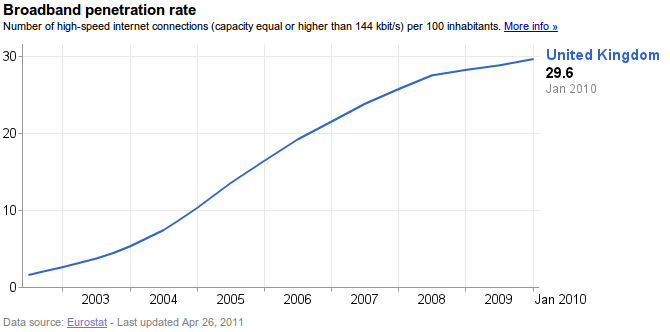
\includegraphics[width=0.45\textwidth]{images/BT-DSL-growth.png}
 \caption{Growth in Broadband connections in the UK}
 \label{fig:bt-dsl-stats}
\end{figure}

For other users, Digital Subscriber Lines (DSL) built on top of the existing plain old telephone system (POTS\nomenclature{POTS}{Plain Old Telephone Service}) are often the only option for anything approaching high-speed internet access. As such, DSL has been a focus of research and development, leading to significant growth in achievable data rates, from 8MBits Downstream for Asymmetric DSL (ADSL\nomenclature{ADSL}{Asymmetric Digital Subscriber Lines}) , through 24 MBits Downstream for ADSL2/2+, and more recently, up to 100MBits symmetrically on short loop lengths (less than 250m) for Very high bit-rate DSL (VDSL\nomenclature{VDSL}{Very high bit-rate Digital Subscriber Lines}).

FTTx and xDSL are both evolving together; as FTTx reduces the last-mile length, xDSL frequency use expands to provide the maximum bandwidth on that short-loop. While in some urban areas, FTTH will become the prevalent form of broadband internet access, xDSL will still be needed for a long time to come for the vast majority of the populace.

But existing methods of managing the bandwidth allocations for bundles of xDSL lines are either computationally simple, but sub-optimal, or computationally intractable and near-optimal. Much work and research has gone into developing advanced and intelligent Dynamic Spectrum Management (DSM) algorithms, but little attention has been applied to the practical implications of these algorithms and the real-world effect that different forms of that implementation make to performance and tractability.

Massively parallel computing, in the form of GPGPU, is becoming a popular paradigm in computational research, with classically linear algorithms being distributed across these Single Instruction Multiple Data (SIMD) devices giving general speed-ups in the range of 5-500x. The most popular and developed form of GPGPU architecture is NVidia's Compute Unified Device Architecture (CUDA\nomenclature{CUDA}{Compute Unified Device Architecture}), which leverages the streaming multiprocessor (SM\nomenclature{SM}{Streaming Multiprocessor}) and high speed memories of their GPU's (usually used for gaming) for use as scientific computation devices. 

In this report, the viability of GPGPU accelerated DSM algorithms is investigated, 
\clearpage
\section{Project Specification}
\label{sec:proj-spec}
\begin{centering}
\textbf{School of Electrical and Electronic Engineering and Computer Science\\
FINAL YEAR PROJECT 2010/2011\\}
\end{centering}

\begin{tabular}{rl}
\\\\Title:&High-Speed bit-loading algorithms for Dynamic Spectrum Management in ADSL\\
Student:&Andrew Bolster\\
Supervisor:&Prof A Marshall\\
Moderator:&Dr J McAllister\\
Area:&Digital Comms\\
Research Cluster:&Digital Comms\\\\
\end{tabular}

Digital subscriber lines need to employ bit-loading techniques to improve their throughput; this is known as “Dynamic Spectrum Management” (DSM). Currently all implementations of DSM use level 1 whereby individual lines use a “water-filling” algorithm to adjust the power allocated to each tone in the spectrum, and a central management station adjusts the water-filling parameters for each line in the subscriber bundle. However this approach is sub-optimal whenever the capacity of the overall bundle is considered, hence more recent research has proposed (level 2) more intelligent methods to allocate the power for each bit in each tone, considering both near and far end crosstalk in the bundle.
A major problem with the level 2 techniques is their computational complexity which currently renders them practically infeasible, e.g. ISB typically takes more than 1 week to compute the tones for a 10-line bundle. Graphic Processing Units (GPUs) represent a new approach to massively parallel floating-point computations. Moreover the Compute Unified Device Architecture (CUDA) developed by NVidia,represents a framework whereby new highly parallel algorithms can be developed. The main aim of this project is to apply this approach to level 2 DSM algorithms, many of which are highly parallel in their operation.

\textbf{The objectives of the project are:}
\begin{enumerate*}
 \item Become familiar with DSM techniques for Digital Subscriber Lines.
 \item Become familiar with the CUDA environment for GPU's and identify a suitable platform.
 \item Investigate efficient implementations of level 2 DSM.
 \item Develop an implementation of a level 2 bit-loading algorithm using GPU's.
\end{enumerate*}

\textbf{M.Eng. Extensions}
\begin{enumerate*}
 \item Analyse the performance of your implementation in terms of speed, cost, and scalability (number of lines).
 \item Compare your design with existing implementations.
\end{enumerate*}

\textbf{Learning Outcomes}
\begin{enumerate*}
 \item Understand how to use CUDA to programme GPU's.
 \item Be able to design bit-loading algorithms for DMT.
 \item How to analyse the performance of an implementation.
\end{enumerate*}

\section{Overview and Objectives}
\label{sec:overview}
The project specification is quite expansive, covering a vast range of areas that I have not encountered directly in my studies but have tangentially met externally. Parallel computation is an active area of research, especially Massively Parallel GPGPU systems such as this. Additionally, there are almost as many DSM algorithms as there are DSM researchers, so algorithm selection and implementation must be very carefully planned and executed to keep within a workable time-frame.

As with any project of this scale, the necessary first stage is a thorough investigation of the problem. Not only the areas of DSM directly relevant to the Level 2 algorithms under analysis, but also the underlying DSL technology to enable generation and implementation of a computational model on which to test the algorithms. This will necessitate the selection of a programming environment that must be held consistent throughout the project, as well as the additional implementation of Optimal Spectrum Balancing (OSB) for comparative analysis. In the interests of not reinventing the wheel, research will also be undertaken to assess the usefulness of any existing DSL models / DSM implementations in terms of development guidance.

Beyond the problem itself, technologies involved in the suggested solution will have to be expansively researched, such as CUDA, GPGPU, and Computational Parallelism, including any recent relevant scholarly works that could be useful.

To summarise, the main points that need investigation will be:

\begin{itemize*}
 \setlength{\itemsep}{0.75pt}
 \setlength{\parskip}{0pt}
 \setlength{\parsep}{0pt}

 \item Problem Research
  \begin{itemize*}
   \item How DSL works
   \item DMT communications
   \item Dynamic Spectrum Management
   \item DSM Levels
   \item Existing/previous DSL simulation systems
   \item Existing/previous DSM implementations
  \end{itemize*}
 \item Solution Research
  \begin{itemize*}
   \item Relevant Programming Environments
   \item Software Profiling
   \item Massively Parallel Computing
   \item Parallel Computing Architectures
   \item CUDA software considerations
   \item CUDA hardware considerations
  \end{itemize*}
 \item Development
  \begin{itemize*}
   \item Design and implement DSL system model simulator
   \item Implement Optimal Spectrum Balancing (OSB\nomenclature{OSB}{Optimal Spectrum Balancing}) algorithm
   \item Implement Greedy bit-loading algorithm (MIPB\nomenclature{MIPB}{Multi-user Incremental Power Balancing, aka Greedy}) algorithm
   \item Implement Iterative Spectrum Balancing (ISB\nomenclature{ISB}{Iterative Spectrum Balancing}) algorithm
   \item Evaluate system performance through the use of profilers and workload visualisation
   \item Develop single-device GPU versions of above algorithms
   \item Evaluate performance of these algorithms, with respect to CPU\nomenclature{CPU}{Central Processing Unit}-bound versions
   \item If viable, implement multi-GPU versions of above algorithms
  \end{itemize*}
 \item Analysis
   \begin{itemize*}
    \item Compare and contrast performance concerns and resource usage of differing implementations
    \item Evaluate system cost concerns, and potential future avenues of development.
   \end{itemize*}
\end{itemize*}

\chapter{Research \& Background}
\label{fig:sec:research}
The modern Broadband telecommunications network has augmented the already massive effect on society of The Internet, allowing access to information from all over the world to one's doorstep. Broadband roll-out and specifically xDSL\nomenclature{xDSL}{Catch-all term for variety of DSL systems} has spurred the growth of VoIP technologies, Video chat and streaming services, and always-on connectivity, fundamentally changing how society interacts; in 2010, over 31 million adults in the UK made purchases online, that's 62\% of the adult population buying from Amazon, Tesco Direct, and eBay instead of going to brick-and-mortar retailers.\cite{OfNS10} 

Almost 30\% of the UK have access to 'Broadband' networks; defined as having a downstream bandwidth of 144Mbits,  triple the number from just five years previously. Nielsen reports that in 2010, over 82\% of the population had some form of internet access available to them; this number up from just under 60\% over the same period.

In terms of speed, variability is rife within the British Isles. Ofcom, in its 2010 year-end report \cite{OfC} finds that while advertised and actual ADSL speeds are up 5\% between May and December 2010, the disparity between advertised 'up to' speeds does not accurately reflect real-world performance. It can be assumed that this disparity can at least be partially explained by service providers using the theoretical capacity of a DSL network, but that network itself cannot adapt to local conditions. The major component of the growth observed in the modern 'to the home' internet is, in Ofcom's opinion, the adoption of new high-speed local-loop technologies, delivering speeds up to and in excess of 45 Mbps in urban areas.

While this is due to a variety of technologies, xDSL plays a massive role; as FTTx technologies increase the available back-haul bandwidth, xDSL technologies are still needed for the ever-shortening (and ever faster) local subscriber loop. Indeed, it is forecast that by 2012, only 4\% of Broadband connections with be complete FTTx lines from subscriber to provider. DSL is still alive and well, and this paper will show that there is still plenty of capacity in existing lines that, if used efficiently, can keep up with subscriber demand for at least the next five years.

\section{DSL}
Digital Subscriber Line networks were originally part of the 1984 ISDN specification. But like most communications technologies, it draws its basis from Claud Shannon's 1948 work at Bell Labs.\cite{CS48}. DSL operates by overlaying wideband digitally modulated data signals on top of existing baseband voice signals on the POTS; over the phone line. This overlaid signal does not effect the voice service, as DSL uses frequencies from around 4kHz to as high as 4MHz; well above the 300-3400Hzoccupied by baseband voice, so both operations can be one asynchronously and simultaneously with little to no interference from each other\footnote{the POTS service can affect the performance of a DSL service if the phone lines are not low-pass filtered and split, but this is now common practise \cite{TS03}}

\subsection{DSL Modulation and Signal Transmission}
Orthogonal Frequency-Division Multiplexing (OFDM\nomenclature{OFDM}{Orthogonal Frequency-Division Multiplexing}), or as it is standardised within DSL\cite{JACB90}, Discrete Multi-Tone (DMT\nomenclature{DMT}{Discrete Multi-Tone modulation}), is the most common modulation scheme in xDSL, where by a large number of orthogonal (non-interfering) sub-channels, tightly packed in the frequency domain, are used to carry data. Across these numerous sub-channels, data is effectively carried in parallel, and streaming data is encoded and split up across these sub-channels at a relatively low symbol rate\cite{JMC91}. In the case of xDSL, this is generally in the range of 2-15 bits per sub-channel\cite{TS03}.

OFDM is used in a wide variety of wideband communications systems, including 802.11a/g/n, WiMax, and DVB-T/H as well as xDSL, and provides many advantages to service providers\cite{VAR};

\begin{enumerate}
  \item Tolerant of Multi-path effects such as fading, and Inter-Symbol Interference (ISI)
  \item Tolerant of narrow-band co-channel interference.
  \item Comparatively high spectral efficiency against spread spectrum modulation systems.
  \item Efficiently implemented using Fast Fourier Transform (FFT)
  \item Run-time adaptable to severe channel conditions without advanced equalisation techniques.
\end{enumerate}

  But it is to be noted that OFDM suffers from some disadvantages;

\begin{enumerate}
  \item Doppler shift sensitivity
  \item Highly sensitive to synchronisation issues
  \item Poor power efficiency due to a High Peak to average power ratio (PAPR) necessitating linear transmission circuitry
\end{enumerate}

The ITU\nomenclature{ITU}{International Telecommunications Union} G.992 specifications, or G.DMT are the ITU specified sub-schemas of OFDM that are used in Asynchronous DSL deployments (ADSL, ADSL2, and ADSL2+), and ITU G.993 specifies the newer Very-high-bit-rate DSL technologies (VSDL, VSDL2). 

  Other xDSL systems such as HDSL, IDSL, RADSL, SDSL, and SHDSL use a combination of Carrier-less Amplitude Phase (CAP) and Two Binary One Quaternary (2B1Q) modulation schemes, which are not the subject of this report, but are interesting to investigate none the less.

  Carrier-less Amplitude Phase modulation was the de facto scheme for ADSL up until around 1996\cite{Sal03}, and was almost completely abandoned for ADSL after the 1999 ratification of ADSL ITU G.992.1 Interoperability standard, but lives on in Rate Adaptive DSL (RADSL), and some HDSL and SDSL deployments.

  Two Binary One Quaternary modulation, as the name indicates, uses four signalling levels to represent a two bit, Gray coded input signal, meaning that if a signal was misread by one-level, only one bit error would occur. In xDSL, 2B1Q is used in ISDN over DSL (IDSL), and some flavours of HDSL and SDSL. 

  As stated, the DMT system as implemented in most A/VDSL systems, operates across hundreds of sub-channels, or slices of the frequency spectrum. How the streaming input data is multiplexed, quantised, and modulated across these sub-channels is largely variable. This Spectrum Management problem will be dealt with in more detail later in this report, but for now, it is suffice to say that data can be dynamically spread across and away from 'poor', noisy sub-channels, and also can be concentrated on 'good', clean areas of the spectrum. This technique is called bit-loading, and entails the use of bit-variable modulation, usually based around variable constellation Quadrature Amplitude Modulation\cite{WW95}, and is demonstrated in the two diagrams in figure ~\ref{fig:QAM_examples}. 

\begin{figure}[h!]
  \centering
  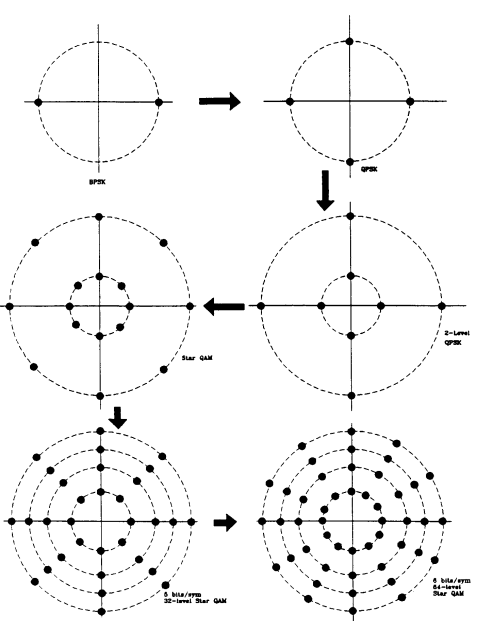
\includegraphics[width=0.45\textwidth]{images/variable_qam.png}
  \caption{Some QAM constellations used in the variable level scheme}
  \label{fig:QAM_examples}
\end{figure}

The capacity of a single DMT line is well established, coming again from Shannon's seminal work\cite{CS48}. His 'ideal' solution, 'Water-filling', simply assigns bit-loads based on the SNR inverse of the line; pouring energy into sub-channels with the best SNR\nomenclature{SNR}{Signal to Noise Ratio}, i.e. most capable of carrying the signal. As the 'best' sub-channels are filled, the adjoining, less capable channels are filled, and so on until no more energy can be added to the channel. 

This is an ideal approach, and presents the maximum theoretical capacity of the line. Practical implementations of this, or any other bit-loading algorithm, must sacrifice 'optimality' for reliability. As such, they must implement what is called a 'Shannon Gap' or 'SNR Gap', a sub-ideal limit on the power loaded on a channel to maintain reliable communications. This subject is revisited in section \ref{sec:XTmodel}, but for the time being, any M-QAM\nomenclature{QAM}{Quadrature Amplitude Modulation} sub-channel constellation, the number of bits that can be encoded within is given in equation ~\ref{eq:MQAMb}\cite{CS48}.

\begin{equation}\label{eq:MQAMb}
b=log_2(M)
\end{equation}

But before going too deeply into the 'problem', first an exploration of the landscape within which the problem lies.

\subsection{DSL System Architecture}
A classical DSL local loop architecture involves a Central Office (CO\nomenclature{CO}{Central Office}), with many Line Termination (LT\nomenclature{LT}{Line Termination, at CO side}) modems,  each connected to a Network Termination (NT\nomenclature{NT}{Network Termination, at CP side}) modem at the Customer Premises (CP\nomenclature{CP}{Customer Premises}). Each LT/NT pair has a separate line between them, and for local loops, these lines are wrapped together in bundles of up to fifty individual lines. This bundle then runs from the CO to the CPs, with intermediate CP lines 'peeling off' the bundle. Additionally, along the length of the bundle, additional lines can 'peel in' to the bundle. Some of the wide variety of possible situations are shown diagrammatically in figures \ref{fig:2-3k5k-nearfar},\ref{fig:4-3k5k-nearfar}.

\begin{figure}[h!]
  \centering
  \subfloat[Possible two line configuration]{\label{fig:2-3k5k-nearfar}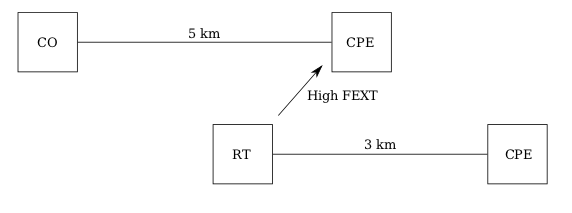
\includegraphics[width=0.45\textwidth]{images/2-3k5k-nearfar.png}}\\
  \subfloat[Possible four line configuration]{\label{fig:4-3k5k-nearfar}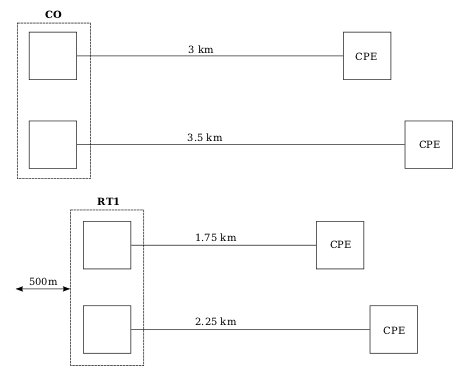
\includegraphics[width=0.45\textwidth]{images/4-3k5k-nearfar.png}}
\end{figure}

These bundles make for a highly noisy RF\nomenclature{RF}{Radio Frequency} environment; with signals from each line interfering with every other line in the bundle through electromagnetic induction of leaked signal power. This phenomenon is termed cross-talk and is the major limiting factor on the achievable data rates of DSL roll-outs, with no current practical solution.

Crosstalk reduces the SNR on DMT sub-channels on a 'victim' line, reducing the amount of bits-per-symbol that can be transmitted on that sub-channel at a pre-defined constant error rate. The level of SNR reduction is often in the 10-20dB range and as such, is the most dominant noise source experienced within the bundle.\cite{RC04}

This phenomenon comes in two major forms; 
\begin{itemize}
  \item Near-End Crosstalk (NEXT\nomenclature{NEXT}{Near End Cross-Talk}): signal leakage from LT-LT or NT-NT
  \item Far-End Crosstalk (FEXT\nomenclature{FEXT}{Far End Cross-Talk}): signal leakage from LT-NT or LT-NT
\end{itemize}

In the vast majority of current DSL roll-outs, NEXT is effectively eliminated through the use of Frequency Division Duplexing(FDD\nomenclature{FDD}{Frequency Division Duplexing}); i.e the upstream data (NT to LT) is sent on a very different frequency than the downstream (LT to NT), and as such does not cause direct interference with a 'neighbouring' termination point.

The amount of cross-talk (XT\nomenclature{XT}{Cross-Talk}) is generally time-constant (excluding severe temperature and humidity changes) and as such can be computationally 'accommodated for' a-priori, but direct vectorisation (we'll find out about that later) and even in-direct cross talk elimination is computationally difficult, if not intractable.

Before one can understand the effects of XT on a DSL system, and especially before one can experiment with different cross talk 'avoidance' algorithms, a realistic dynamic simulation of a functional DSL system must be generated. 

\subsubsection{DSL System Modelling}
Modelling a DSL system, instead of opting for 'real-world' values, allows experimentation and observation of channel behaviours that may not be immediately clear from end-point experimentation \footnote{not to mention that real-world experimentation is time-consuming, expensive, and often incomparable to other results due to a multitude of measurement standards}

Simulation in this case involves the generation of a cross-talk gain (XTG\nomenclature{XTG}{Cross Talk Gain}) matrix for an \(N\)-line network for each of its \(K\) operating channels. This XTG matrix will then be used by the management algorithms to assess the 'cost' or indeed viability of a particular bit-load on a particular line on a particular channel.

As such it is important to understand the electromagnetic transmission characteristics of twisted pair phone lines. This area is largely concerned with the generation of per-line-per-channel transfer functions for interacting sections within a bundle. It is shown in \cite{TS99} that for standard (Category 3) lines, the following RLCG characterisation is stable up to the 30MHz area, at which point this 'simplified' characterisation veers away from real-world performance due to high-frequency envelope shearing. Category 5 lines are stable with this kind of characterisation up to around 150MHz. 

RLCG Characterisation is derived from the per-unit-length two-port model shown in figure ~\ref{fig:rclg}, which can be viewed as a infinitesimally small section of a segment of transmission line. The RCLG parameters represent Resistance, Inductance, Capacitance and Conductance per unit length of line. The direct gain channel models used in this report are based on the long line approximations taken from \cite{AM09}, which in turn were taken from \cite{TS99}.

\begin{figure}[h!]
  \centering
  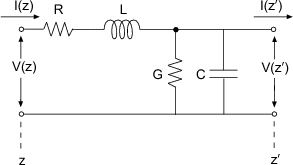
\includegraphics[width=0.25\textwidth]{images/rclg.png}
  \caption{RCLG Characterisation of a two port linear network}
  \label{fig:rclg}
\end{figure}

This assumption is that (for a long DSL line) the input line impedance \(V_1\) matches the characteristic impedance \(V_2\). Given that assumption as well as;
\begin{itemize}
\item \(d\) :line length
\item \(Z\) :Impedance per unit length:\(R \cdot L\)
\item \(Y\) :Admittance per unit length: \(G \cdot C\)
\item \(Z_l\) :load impedance
\item \(Z_s\) :source impedance
\item \(Z_0\) :characteristic impedance:\(\sqrt{\frac{Z}{Y}}\)
\item \(\gamma\) :propagation constant:\(\sqrt{Z \cdot Y}\)
\end{itemize}

The transfer function for a given DSL line is;

\begin{equation}\label{eq:DSLTransferFunc}
H=\frac{Z_0 \cdot \text{sech}(\gamma d)}{Z_s \cdot [\frac{Z_0}{Z_1} +\text{tanh}(\gamma d)]+Z_0 \cdot[1+\frac{Z_0}{Z_1} \cdot \text{tanh}(\gamma d)]}
\end{equation}

To ensure that this modelled transfer function is smooth with respect to frequency \footnote{necessary due to the large margins of error in characterising 'real-world' lines}, the RLCG values are parametrised thus;

\begin{equation}\label{fig:R}
R(f) = \frac{1}{\frac{1}{\sqrt[4]{r^4_{0c}+a_c\cdot f^2}} + \frac{1}{\sqrt[4]{r^4_{0s}+a_s\cdot f^2}}}
\end{equation}

Where \(r_{0x}\) is the DC resistance of copper (c) and steel (s) and \(a_x\) are skin effect related constants

\begin{equation}\label{fig:L}
L(f) = \frac{l_0+l_{\infty}(\frac{f}{f_m})^b}{1+(\frac{f}{f_b})^b}
\end{equation}

Where \(l_x\) are low (0) and high (\(\infty\)) frequency inductance and \(b\) and \(f_m\) define the transition from low to high frequencies.

\begin{equation}\label{fig:C}
C(f)= c_{\infty} + c_0 \cdot f^{-c_e}
\end{equation}

Where \(C_x\) represent contact (\(\infty\)) and other (\(0,e\)) capacitances, chosen from measurements.

\begin{equation}\label{fig:G}
G(f)=g_0\cdot f^{+g_e}
\end{equation}

Where \(G_x\) represent (\(0,e\)) conductances, chosen from measurements.

Within this project, as in \cite{AM09}, AWG 24 line parameters were used, shown in table ~\ref{tab:AWG24Tbl}.

\begin{figure}[h!]
  \centering
  \begin{tabular}{|c|c|c|c|}\hline
    \(r_{0c}=174.56 \Omega\)/km&\(r_{0s}=\infty \Omega\)/km&\(a_c=0.0531\)&\(a_s=0.0\)\\\hline
    \(l_{0}=617.25 \mu H\)/km&\(l_{\infty} = 478.97 \mu H\)/km&\(b=1.1529\)&\(f_m=553.76\)kHz\\\hline
    \(c_{\infty} = 50 \mu F\)/km&\(c_0=0.0\mu F\)/km&\(c_e=0.0\)&\\\hline
    \(g_0 = 234.874 fS\)/km&\(g_e=1.38\)&&\\\hline
  \end{tabular}
  \caption{ETSI Parameters used for AWG24 coaxial lines}
  \label{tab:AWG24Tbl}
\end{figure}


Using these parameters, figure ~\ref{fig:XTG_Example} shows the gain-curve for a variety of lengths of AWG24 cabling produced from equation ~\eqref{eq:DSLTransferFunc}

\begin{figure}[!h]
  \centering
  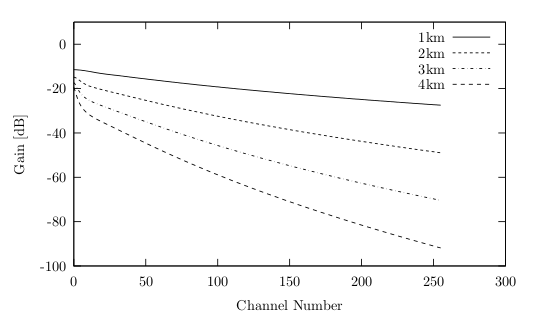
\includegraphics[width=0.45\textwidth]{images/awg24lengths.png}
  \caption{Gain versus channel model for a range of transmission lengths}
  \label{fig:XTG_Example}
\end{figure}

\subsubsection{Crosstalk Modelling}
\label{sec:XTmodel}

The above model allows the generation of 'idealised gains' for a given line, ignoring all external effects, such as the aforementioned cross-talk. To bring cross-talk into the picture, assuming that NEXT is eliminated completely by FDD, we can model FEXT based on the industry standard ETSI 1\% \cite{ETSI03} model (equation ~\eqref{eq:ETSIFEXT})

\begin{equation}\label{eq:ETSIFEXT}
|H_{FEXT}(f)|^2=N^{0.06}K_{FEXT}f^2 |H_{channel}(f,L)|^2
\end{equation}

The "1\%" in this case represents the worst-case-scenario, and in a real deployment would not be encountered 99\% of the time. This is partially driven from systemic pessimism, but partially comes from the fact that this worst-case scenario allows for a modelling function that is smooth with frequency.

In most cases, this 1\% model is over zealous in its estimations of cross-talk coupling, and also ignores spatiality within the bundle \footnote{i.e., lines in the core of the bundle receive much more cross-talk than those on the skin of the bundle}. Using real data from a four sub-bundle, 100x100 DSL binder, the existing model can be modified to more closely match the coupling data of the 'real' bundle.

\begin{equation}\label{eq:ATTFEXT}
|H^{j,k}_{FEXT}(f)|^2=|H^{j,k}_{FEXT}(f)|^2 \times 10^{\frac{X_{dB}}{10}}
\end{equation}

Where the modifier \(X\) is selected based on a Beta probability distribution of sample data, for example, \cite{Alc07}.

As stated, DSL is a cross-talk-limited system, and as such, the effect of cross-talkers also effects some of the fundamental assumptions that must be made about the transmission characteristics of the lines in the bundle.

From \cite{SJ08}, the approximate Shannon Gap for a DSL system based on M-QAM is derived thus. From the Central Limit Theorem, as the number of cross-talkers increases, the effects of those cross-talkers approximates to a Gaussian Distribution\cite{KK93}. Therefore, a DSL channel can be approximated as an Additive White Gaussian Noise (AWGN) channel, which is described \cite{CS48}:

\begin{equation}\label{eq:AWGN}
C(k)=log_2(1+SNR(k))
\end{equation}

This represents the maximum possible capacity (in bits) on a given channel (\(C(k)\)), ignoring practical considerations such as coding complexity and processing delays. From \cite{CS48} and \cite{JMC91}, the probability of a symbol error for an uncoded M-QAM constellation \footnote{with an associated number of nearest neighbours, \(N_e\)} on a given sub-channel is shown in equation ~\eqref{eq:PeMQAM}

\begin{equation}\label{eq:PeMQAM}
P_e\approx N_eQ\left(\sqrt{\frac{3}{M-1}SNR}\right)
\end{equation}

Where \(Q(x)\) is the probability of unitary Gaussian variable will will exceed \(x\), given in equation ~\eqref{eq:QxQAM}. In general, DSL systems aim for this probability of symbol error (\(P_e\)) to be around \(1e^{-7}\).

\begin{equation}\label{eq:QxQAM}
Q(x)=\int_x^{\infty}\frac{1}{\sqrt{2\pi}}e^{-u^2/2} du
\end{equation}

\eqref{eq:QxQAM} is generally rewritten in terms of the standard error function \(erf(x)\), shown in equations ~\eqref{eq:QxQAMerf} and ~\eqref{eq:QxQAMerf2}.

\begin{equation}\label{eq:QxQAMerf}
Q(x)=\frac{1}{2}\left(1-erf(\frac{x}{\sqrt{2}})\right)
\end{equation}

\begin{equation}\label{eq:QxQAMerf2}
Q^{-1}(x)=\sqrt{2} erf^{-1}(1-2x)
\end{equation}

Rearranging ~\eqref{eq:PeMQAM} for \(M\) gives ~\eqref{eq:QAM4M}

\begin{equation}\label{eq:QAM4M}
M=1+\frac{SNR}{\frac{1}{3}(Q^{-1}(\frac{P_e}{N_e})^2)}
\end{equation}

Revisiting ~\eqref{eq:MQAMb}, ~\eqref{eq:MQAMbmax} can be obtained, expressing the number of bits that can be encoded on a sub-channel.

\begin{equation}\label{eq:MQAMbmax}
b=log_2\left(1+\frac{SNR}{\frac{1}{3}(Q^{-1}(\frac{P_e}{N_e})^2)}\right)
\end{equation}

Contrasting ~\eqref{eq:MQAMbmax} with ~\eqref{eq:AWGN}, the uncoded channel gap is defined in equation ~\eqref{eq:GAMMAuncoded}.

\begin{equation}\label{eq:GAMMAuncoded}
\Gamma_{uncoded}=\frac{1}{3}\left(Q^{-1}(\frac{P_e}{N_e}\right)^2
\end{equation}

This allows simplification of equation ~\eqref{eq:MQAMbmax} with respect to ~\eqref{eq:GAMMAuncoded} into ~\eqref{eq:GAMMAb}

\begin{equation}\label{eq:GAMMAb}
b=log_2\left(1+\frac{SNR}{\Gamma_{uncoded}}\right)
\end{equation}

This characterisation of the Shannon Gap is not quite complete, and represents the best-case scenario within a DSL system, while ignoring potential coding gains from Forward Error Correction such as the Trellis\cite{GU82} or Reed-Solomon\cite{Ree59} coding schemes.

As such, two additional modifiers are added to the \(\Gamma\) calculation; a performance margin \(\gamma_m\) which allows for SNR 'headroom' to maintain error rates during temporarily bad noise conditions, and a coding gain \(\gamma_{eg}\) which incorporates any error correction modulation in place. This gives a final \(\Gamma\) sum shown in equation ~\eqref{eq:GAMMAsum}

\begin{equation}\label{eq:GAMMAsum}
\Gamma=\Gamma_{uncoded}+\gamma_m+\gamma_{eg}
\end{equation}

In \cite{AM09} it is demonstrated that cross-talk coupling can be assumed not to have any practically relevant effect on sub-channels other than the sub-channel from which that cross-talk originates, such as when DMT blocks are transmitted and received synchronously or when cyclic prefixing and pulse shaping ("Zipper" DMT\cite{FSJ99}) is used.

From \cite{CA06}, equation ~\eqref{DSLSystemModel} shows the maximally optimal bit-loading on line \(n\) of \(N\) users, and tone \(k\) of \(K\) total sub-channels, including the above derivation for FEXT coupling.

\begin{equation}\label{DSLSystemModel}
b_n(k)=log_2\left(1+\frac{p_n(k) |h_{nn}(k)|^2}{\Gamma \left( \sigma_n^2(k)+\sum_{j\neq n}^N p_j(k)|h_{jn}(k)|^2 \right)} \right)
\end{equation}

In equation ~\eqref{DSLSystemModel}, the following definitions are provided for clarity;

\begin{itemize}
  \item \(h_{ij}(k)\)\nomenclature{\(h_{ij}(k)\)}{XTG from user \(i\) to user \(j\) on channel \(k\) }:The cross-talk gain from user \(i\) to user \(j\) on channel \(k\)
  \item \(p_n(k)\)\nomenclature{\(p_n(k)\)}{Power provisioned on channel \(k\) for user \(n\)} :The power provisioned on channel \(k\) for user \(n\)
  \item \(\sigma^2_n(k)\)\nomenclature{\(\sigma^2_n(k)\)}{Background noise power experiences by user \(n\) on channel \(k\)} :The background noise power experienced by user \(n\) on channel \(k\)
  \item \(\Gamma\)\nomenclature{ \(\Gamma\)}{The Shannon Gap derived from equation \eqref{eq:GAMMAsum}}:The Shannon Gap derived from ~\eqref{eq:GAMMAsum}
\end{itemize}

By letting \(f(b_n(k))=\Gamma(2^{b_n(k)}-1)\), ~\eqref{DSLSystemModel} can be rearranged to ~\eqref{eq:DSLSystemModelAlt}

\begin{equation}\label{eq:DSLSystemModelAlt}
p_n(k)-f(b_n(k))\sum_{j\neq n}^N p_j(k) \frac{|h_{jn}(k)|^2}{|h_{nn}(k)|^2}=f(b_n(k))\frac{\sigma_n^2(k)}{|h_{nn}(k)|^2}
\end{equation}

It is clear that equation ~\eqref{eq:DSLSystemModelAlt} can be characterised as an N-dimensional linear system of equations, of the form 

\begin{equation}\label{eq:SysModMat}
A(k)P(k)=B(k)
\end{equation}

Where

\begin{equation}\label{eq:SysModA}
A(k)_{ij}=\begin{cases} 1, & \mbox{for } i = j \\\frac{-f(b_i(k))|h_{ji}|^2}{|h_{ii}|^2}, & \mbox{for } i \neq j \end{cases}
\end{equation}

\begin{equation}\label{eq:SysModP}
P(k)=[p_1(k) \dots p_i(k) \dots p_N(k)]^T
\end{equation}

\begin{equation}\label{eq:SysModB}
B(k)=\left[\frac{f(b_1(k)) \sigma^2_1}{|h_{11}|^2} \dots \frac{f(b_i(k)) \sigma^2_i}{|h_{ii}|^2} \dots \frac{f(b_N(k))\sigma^2_N}{|h_{NN}|^2}\right]^T
\end{equation}

As such, the vector \(B(k)\), as a function of \(b(k\), describes the amount of bits loaded onto each user's line on tone \(k\), and \(P(k)\) prescribes the power required on each line to support the vector \(B(k)\) of bits loaded onto those lines on channel \(k\). It is the solution and optimisation of this system of equations that is the fundamental limiting factor, and drive for, DSM systems. 

The reasoning for this is primarily visible looking at the concept of rate-regions, i.e an \(N\)-dimensional surface of possible maximum line bit-loads for each user \(n\). Figure ~\ref{fig:RateRegionExample} shows the relationship between two given users, \(R_1\) and \(R_2)\) within a given bundle. It is evident that one \emph{could} achieve an very high data-rate on one line, but at great expense to the other. Mathematically, the search for optimal bit-loading is summed up in ~\eqref{fig:RateRegionEqu}.

\begin{figure}[h!]
  \centering
  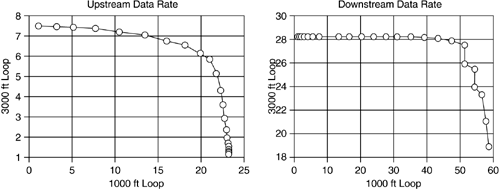
\includegraphics[width=0.75\textwidth]{images/rateregion.png}
  \caption{Example of a ADSL rate Region for two users from \cite{TS03}}
  \label{fig:RateRegionExample}
\end{figure}

\begin{equation}\label{fig:RateRegionEqu}
\max\limits_{\{p_n\in P_n\}_n} \sum_n w_n R_n
\end{equation}

Using an optimal rate-region, of the style demonstrated in equation ~\ref{fig:RateRegionEqu} can be generated algorithmically from the above equations. But often these algorithms can be computationally intractable, and less computationally expensive (but sub-optimal) algorithms are used instead, producing reduced rate regions which do not take full advantage of the available spectrum given the same cross-talk and bundle noise characteristics.

In essence, this Spectrum Management Problem, as stated in equation ~\eqref{fig:RateRegionEqu}, can be expanded based on line-weighting; where some lines get 'preferential treatment', either because they are paying more, or as part of a lead-and-lag rate-compensation system\footnote{Lag and Lead, terms originally from the field of economics but 'adopted' by the field of control theory, implies a kind of 'lending' system, where by a given variable (in this case the bit-rate/weight on a particular line) can be allowed to 'run rampant' if the system has spare capacity, but that added usage is accounted and is 'paid back' to the system when needed, and often that particular variable will be more 'borrowed from' until its lag/lead accounts are even again}. Thus, the Spectrum Management Problem can be generalised to \(N\) users as a maximisation of a weighted sum of data rates within a bundle, as shown in equation ~\eqref{fig:WeightedDSLSystemModel}.

\begin{equation}\label{fig:WeightedDSLSystemModel}
\begin{array}{rc}
\sum\limits_{n=1}^N w_n \sum\limits_{k=1}^K & log_2 \left(1+\frac{p_n(k_|h_{nn}(k)|^2}{\Gamma\left(\sigma_n^2(k)+\sum\limits_{m\neq n}^N p_m(k)|h_{jm}(k)|^2\right)}\right)\\
 &s.t.\sum_{k=1}^Kp_n(k) \leq P_{max,n} \forall n
\end{array}
\end{equation}

The optimisation of this problem in a dynamic near-realtime time-frame is the major focus of DSM research, which is summarised next.


\subsection{Dynamic Spectrum Management Introduction}
A general solution to this rate-region problem has been the use of Static Spectrum Management (SSM), where each line has a pre-defined power spectral density (PSD\nomenclature{PSD}{Power Spectral Density}) profile under which it operates. This is sometimes called Spectral Masking. Unfortunately this masking is done once (or a few times, if lines are added to / removed from the bundle), and additionally assumes that each line will be fully utilised at all times. This a major abstraction from reality, and has driven the development of spectrum management systems that can dynamically re-allocate PSD's based on near-real-time usage. From \cite{STC07}:

\begin{quotation}
Suppose that 25 copper lines exist in a cable bundle. Depending on the time (day versus night, weekday versus weekend) and the location (commercial versus residential area), the demand for DSL services varies. For example, the data traffic load at an office is heavy during the daytime and may be close to zero at night. Furthermore, depending on the specific loop topologies, the interference caused by one line to another varies. Some pairs might be physically close in the binder over a very short distance; hence, the interference between these pairs might be very small. On the other hand, other pairs might be proximate along most of the loop length, which leads to a very strong interference between those two pairs
\ldots
Revisiting the example where 25 copper lines exist in a telephone bundle, suppose that in the middle of the night at school, one Ph.D. student is trying to download a large paper from a website using DSL. If static spectrum management is used, the speed is as slow at night as during the day, when many other students are also using their DSLs. However, if the DSL network uses [Dynamic Spectrum Management], the speed at night can be much faster than during the daytime because the bit-rate on the line in use can be optimised to take advantage of the low-noise conditions.
\end{quotation}

It is clear that with the addition of some usage-based intelligence, the bundle could be much more effectively used. Dynamic Spectrum Management systems allow for power and rate allocations for each line to be dynamically controlled, but are classified into four general levels, based on the amount of coordination between lines, ranging from completely autonomous operation\footnote{Strictly speaking not DSM but included for completeness} to centralised signal vectoring and control, as summarised in Figure \ref{tab:DSMLevelTable}, adapted from \cite{JC06} and \cite{AM09}.

\begin{figure}[h!]
  \begin{minipage}{\textwidth}
\begin{tabularx}{\textwidth}{c|X|p{3cm}|}
  DSM Level&Description&Examples\\\hline
  0&No DSM, Completely Autonomous per-modem Spectrum Management&NA \\
  1&Single line spectrum balancing with politeness and signal impulse control&IWF\footnote{Iterative Water Filling},ASB\footnote{Autonomous Spectrum Balancing}\\
  2&Multiple line spectrum balancing with spectra controls&OSB\footnote{Optimal Spectrum Balancing}, ISB\footnote{Iterative Spectrum Balancing},SCALE\footnote{Successive Convex Approximation for Low ComplExity\cite{Pap06}}\\
  3&Multiple line signal coordination (vectoring)&Vectored-DMT\cite{GG00}, SVD\footnote{Single Vector Decomposition\cite{GTaWH00}}\\
\end{tabularx}
\end{minipage}
\caption{Summary of DSM Algorithm Level Characteristics with Examples}
\label{tab:DSMLevelTable}
\end{figure}


This coordination (where applicable) is controlled centrally from a Spectrum Maintenance Centre (SMC\nomenclature{SMC}{Spectrum Maintenance Centre}), which receives data from Customer Premises Equipment (CPE\nomenclature{CPE}{Customer Premises Equipment}) via an Auto-Configuration Server (ACS\nomenclature{ACS}{Auto-Configuration Server}), and/or from DSLAMs\nomenclature{DSLAM}{DSL Access Multiplexer} and LT-side equipment via an Element Management System (EMS\nomenclature{EMS}{Element Management System}). The SMC then collates the received information, and distributes profile settings for the DSLs.

\subsection{DSM Level 0/1}
For clarity, levels 0 and 1 are generally grouped, as the only major difference is that while in level 0\footnote{currently the most common method of 'Spectrum Balancing'}, equipment is completely autonomous in terms of its own spectrum management; level 1 systems receive power and rate limitations from the SMC, within which they must operate. Level 0 is currently the most commen method of DSM utilised currently, but some ISPs are moving to level 1 systems, such as Virgin.

Thinking back to the initial discussion of DMT spectrum balancing, the most common technique for autonomous spectrum assignments is based on Water-filling \cite{CS48}, and refined for DSL in \cite{WYaJC00} \cite{WY01}

For the single user case, refer to figure ~\ref{fig:WaterFillingSingleExample}, but in the multi-user case, water-filling attempts must be iteratively refined (Hence, Iterative Water-Filling, or IWF\nomenclature{IWF}{Iterative Water-Filling}); so as to allow the 'other' lines to see each lines new noise profile, see figure ~\ref{fig:WaterFillingMultiExample} for a graphical example of this. This helps to reduce the effects of the so-called "Near Far Problem", whereby the received signal from cross-talker which is closer to the receiver, is stronger than its direct line transmitter signal.

\begin{figure}[h!]
  \centering
  \subfloat[Single User]{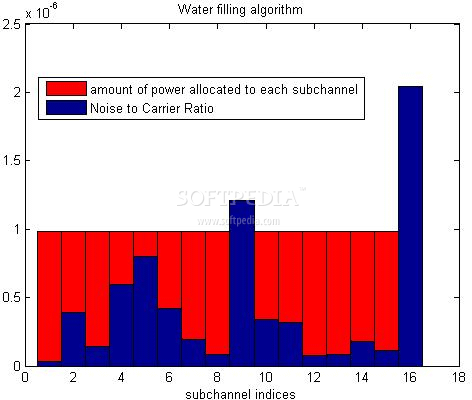
\includegraphics[width=0.5\textwidth]{images/wf.png}\label{fig:WaterFillingSingleExample}}
  \subfloat[Iterative Multiple User]{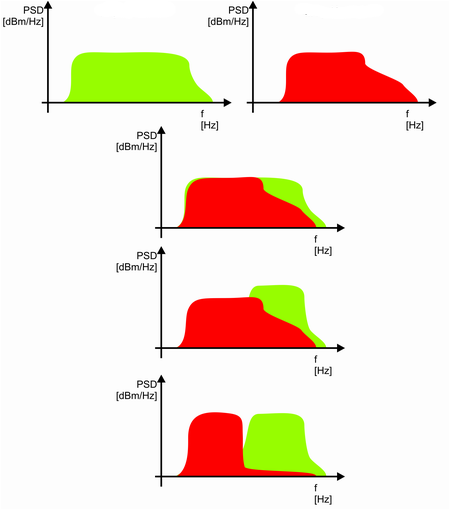
\includegraphics[width=0.4\textwidth]{images/iwf.png}\label{fig:WaterFillingMultiExample}}
  \caption{Example of Water Filling}
\end{figure}

The water-filling algorithm produces the optimal solution\footnote{It is proven in \cite{STC03} that for frequencies less than 2MHz, there exists only one Nash Equilibrium point within a distributed DSL network, and although it is possible, no example of multiple optimal rate-region points has been discovered to date \cite{STC07}}, maximising channel capacity for a single user with a continuous bit-assignment \footnote{I.e non-integer bit-assignments are permitted}. In practise this is incorrect, as integer bits must be assigned to each channel for transmission. When this integer condition is applied, it is known as "Discrete Water-filling". Discrete water-filling has two variations; one which focuses on maximising bit-rate with respect to a stated power budget, known as Rate-Adaptive (RA\nomenclature{RA}{Rate Adaptive water filling}); and another which focuses on minimising the power requirements with respect to a stated bit-rate, known as Fixed-Margin (FM\nomenclature{FM}{Fixed-Margin water filling}). These two conditions are mathematically phrased in ~\eqref{RADefine} ~\eqref{FMDefine}\cite{TS99}.

\begin{equation}
  \begin{array}{rcl}
  max R&=&\sum_{k=1}^Kb(k)\\
  s.t.&&\sum\limits_{k=1}^Kp(k)\leq P_{budget}
  \end{array}
\label{FMDefine}
\end{equation}

\begin{equation}
  \begin{array}{rcl}
  min &&\sum\limits_{k=1}^Kp(k)\\
  s.t.&&\sum\limits_{k=1}^Kb(k)\geq B_{budget}
  \end{array}
\label{RADefine}
\end{equation}

The resolution of both of these forms of water-filling is surprisingly simple in theory; find the tone with the lowest bit-addition energy \footnote{generally termed \(\Delta p(k)\)\nomenclature{\(\Delta p(k)\)}{Single-bit addition power}}, and add a bit to it. This continues until either the power or rate budget is reached, depending on the mode applied. This basic algorithm is the Levin-Campello (LC\nomenclature{LC}{Levin-Campello Algorithm}) Algorithm\cite{H.L01}.

\subsubsection{Iterative Water Filling}
One of the first forms of DSM, IWF is computationally simple, de-centralised, and relatively easy to implement.
The rational of IWF is to limit iteratively perform LC bit-loading and to adapt the power constraints so as to limit the power used in the bundle while maintaining total bundle capacity, thereby lowering the power of cross-talking signals and actually increasing the net bundle data rate greatly when compared to SSM\nomenclature{SSM}{Static Spectrum Management}, but is far from optimal, and is not guaranteed to converge, or settle, on on any result. The general algorithm for IWF is shown in figure \ref{fig:IWFAlgorithm}

\begin{figure}[h!]
\begin{algorithmic}
\REPEAT
\FOR{n=1...N}
\STATE Execute LC Algorithm with power budget \(P_n\) on line \(n\)
\IF{\(R_n>R_n^{target}\)}
\STATE \(P_n=P_n-\gamma\)
\ELSE
\STATE \(P_n=P_n+\gamma\)
\ENDIF
\ENDFOR
\UNTIL{convergence}
\end{algorithmic}
\caption{IWF Algorithm}
\label{fig:IWFAlgorithm}
\end{figure}

\subsection{DSM Level 2}
\subsubsection{Optimal Spectrum Balancing}
From \cite{RC04}, OSB optimally solves the Spectrum Management Problem for multiple users, but is highly computationally intensive and generally cannot be practically computed for more than four lines \cite{AM09}. The avenue taken by OSB in solving the Spectrum Management Problem is a mathematically complex one. The solution is centred around the use of a Lagrangian dual decomposition of the initially states Spectrum Management Problem ~\eqref{fig:WeightedDSLSystemModel}. To explain what this process entails, one must look closer at the problem; from \cite{RC04}

\begin{quotation}
  The fundamental problem is that the total power constraints on the modems couple the optimisation across frequency. As such optimisation must be done jointly across all tones, which leads to an exponential complexity in \(K\). We overcome this problem through the use of the dual decomposition method. This technique allows us to replace the constrained optimisation problem with an unconstrained maximization of a Lagrangian\footnote{A Lagrangian of a dynamical system is a function that summarises the dynamics of the system, and in the field of optimisation, allows for the joint-optimisation of a dually (in this case) constrained problem through the use of an additional Lagrange multiplier to generate the new Lagrangian decomposition \(L\) that implicitly encompasses both (all) constraint functions} The Lagrangian incorporated the constraints implicitly into the cost function, removing the need for the constraints to be explicitly enforces. As a result, the optimisation can be decoupled across frequency, and an optimal solution can be found in a per-tone fashion. This leads to a linear rather than exponential complexity in \(K\) and a computationally tractable problem.
\end{quotation}
 
In practical terms, that means that the Spectrum Management Problem can be 'simplified' to include the pan-channel power constraints, meaning that instead of generating many solutions to the general (first line of ~\eqref{fig:WeightedDSLSystemModel}) problem, and then subsequently discarding those as they do not satisfy the bundle power constraints, global power is a focal consideration. The Lagrangian decomposition of ~\eqref{fig:WeightedDSLSystemModel}, encompassing the power constraints, is shown in ~\eqref{fig:LagrangianModel}

\begin{equation}
L=\sum\limits_{n=1}^N w_n \sum\limits_{k=1}^K log_2 \left(1+\frac{p_n(k_|h_{nn}(k)|^2}{\Gamma\left(\sigma_n^2(k)+\sum\limits_{m\neq n}^N p_m(k)|h_{jm}(k)|^2\right)}\right)-\lambda_n\left(\sum\limits_{k=1}^K p_n(k)\right)
\label{fig:LagrangianModel}
\end{equation}

Is was shown by Yu and Lui\cite{WYaRL06} that this decomposition is an exact match to the originally stated problem for large numbers of channels.

It is also stated in \cite{AM09} that ~\eqref{fig:LagrangianModel} can be tonally decoupled, and a (unfortunately non-convex) Lagrangian expression for each channel generated, as in ~\eqref{fig:LagrangianDecoupled}, and by optimising for a maximal per-tone Lagrangian, and searching \(\lambda\) space\footnote{How the \(\lambda\) space is searched is a matter of much debate, which will be met later}, the original problem can be solved.

\begin{equation}
  L(k)\nomenclature{\(L_k\)}{The Lagrangian sum of a bitloaded channel}=\sum\limits_{n=1}^Nw_nb_n(k)-\sum\limits_{n=1}^N\lambda_np_n(k)
\label{fig:LagrangianDecoupled}
\end{equation}

Since ~\eqref{fig:LagrangianDecoupled} is non-convex, an exhaustive search across \(b_n\) space is required\footnote{For the interested reader, this is a computationally explosive procedure; consider the vector \(B(k)\), with each vector index as the bit load on a particular line on channel \(k\), and a maximum bits per tone of 15 (from the DSL standard). For two lines, this represents only 225 possibilities, but for four, its 50625; for 8 its over 2.5 billion, and for a standard 50 line bundle, its a 59 digit number.To put that in perspective, the number of stars in the observable universe is only a 24 digit number. For a given max bits per tone \(b_{max}\), the number of bit combinations for \(N\) lines is \(b_{max}^{N}-1\)}
Even with the Lagrangian decomposition, the computationally explosive nature of this exhaustive bit-field search renders OSB computationally intractable for more than four or five lines. Some run-times from \cite{AM09} are shown in figure ~\ref{tab:TractibilityTable}

The generalised algorithm for OSB is shown in figure \ref{fig:OSBAlgorithm}

\begin{figure}[!h]
\begin{algorithmic}
\REPEAT
\REPEAT
\FOR{\(k=1\dots K\)}
\STATE \(\arg\max_{b_(k)}L(k)=\sum_{n=1}^Nw_nb_n(k)-\sum_{n=1}^N\lambda_np_n(k)\)
\STATE Solve by N-d exhaustive search
\ENDFOR
\STATE \(\lambda_n=\lambda_n+\epsilon(\sum_{k=1}^Kp_n(k)-P_n^{max})\)
\UNTIL{\(\lambda\) convergence}
\STATE \(w_n=w_n+\epsilon(\sum_{k=1}^Kb_n(k)-R_n^{target})\)
\UNTIL{\(w\) convergence}
\end{algorithmic}
\caption{OSB Algorithm}
\label{fig:OSBAlgorithm}
\end{figure}

OSB can be augmented using a Branch and Bound searching structure into Branch and Bound OSB (BBOSB). BBOSB is covered in detail in \cite{PT06}, but suffice to say, even with the improved searching structure, BBOSB is still exponential in \(N\), but with a lower complexity coefficient; where OSB is only tractable for 4-5 lines, BBOSB is tractable up to approximately 10 lines \cite{AM09}.

\subsubsection{Iterative Spectrum Balancing}
ISB is based on the same Lagrangian decomposition as OSB, but instead of an exhaustive search across the bit-space within the Lagrangian, each line in turn is optimised, i.e a linear search instead of OSB's \(N\)-vector-search. It was presented\cite{Cen05} by Cendrillon and Moonen in 2005 and thoroughly investigated by Yu and Lui\cite{WYaRL06} in 2006, and is near-optimal, but is not guaranteed to converge on a global maximum.\cite{Cen05}.

The improvement in computational complexity is great; OSB has a \(N\) complexity of \(O(b_{\text{max}}^N)\), whereas ISB attains a complexity of \(O(N^2)\), meaning that for slightly more practical bundle sizes, ISB is computationally tractable. The ISB algorithm is shown in figure ~\ref{fig:ISBAlgorithm}

\begin{figure}[h!]
\begin{algorithmic}
\REPEAT
\FOR{\(k=1\dots K\)}
\REPEAT
\FOR{\(n=1\dots N\)}
\STATE Fix \(b_m(k)\forall m \neq n\)
\STATE \(\arg\max_{b_(k)}L(k)=\sum_{n=1}^Nw_nb_n(k)-\sum_{n=1}^N\lambda_np_n(k)\)
\STATE \(\lambda_n=\lambda_n+\epsilon(\sum_{k=1}^Kp_n(k)-P_n^{max})\)
\STATE Solve by 1-d exhaustive search
\ENDFOR
\UNTIL{\(\lambda\) convergence}
\ENDFOR
\STATE \(w_n=w_n+\epsilon(\sum_{k=1}^Kb_n(k)-R_n^{target})\)
\UNTIL{\(w\) convergence}
\end{algorithmic}
\caption{ISB Algorithm}
\label{fig:ISBAlgorithm}
\end{figure}

\subsubsection{Multi-User Greedy Spectrum Balancing}
It has been shown that while the LC algorithm is optimal in the case of a single line, the straightforward multi-user expansion of this (IWF) is decidedly sub-optimal. Cioffi, Sonalkar, and Lee, in \cite{JL05} presented a heuristic extension to the Levin-Campello Algorithm, termed Multi-User Greedy Spectrum Balancing. 
The heuristic applied was, instead of in IWF where each line is individually optimised, the bundle is viewed as a whole, and bits are iteratively assigned to both the line and channel with the minimum cost of addition.
This cost of bit-incrementing, which for IWF was simply \(\Delta p_m(k)\) where \(m\) was the line being balanced, and \(k\) was the channel on the line with the lowest additional power requirement; additionally includes the sum of \(\Delta p_n(k)\) on all other lines required to accommodate the additional cross-talk generated on the incremented line ~\eqref{eq:GreedyCost}.

\begin{equation}
C(m,k)=\sum\limits_{n=1}^N\left(\underset{p_n(k)}{b(k)+1} - \underset{p_n(k)}{b(k)}\right)
\label{eq:GreedyCost}
\end{equation}

\subsubsection{Multi-User Incremental Power Balancing}
In \cite{AM09}, McKinley details the development of MIPB as coming from a critical analysis of Multi-User Greedy Spectrum Balancing. One of the major deficiencies of Greedy is the (significant) possibility of the algorithm getting stuck in local minima, or getting 'deadlocked', whereby bits cannot be added to any lines due to any other line in the bundle attempting to violate  its power constraint to accommodate the additional cross talk incurred, (see ~\ref{eq:GreedyCost}). To remedy this, an adaptive power penalty function is used to stop 'clean' lines being continuously loaded up to their power budget, and then 'locking' all other lines, and to instead force all the lines to be more or less equalised as the algorithm progresses. The algorithm for MIPB is shown in figure \ref{fig:MIPBAlgorithm}. The final bundle efficiency of MIPB, while non-optimal, is very close, but the real improvement is in runtime performance; 10 lines with rate targeting applied in under five minutes.

\begin{figure}[h!]
\begin{algorithmic}
\REPEAT
\STATE \(\text{argmin}_{n,k} C\)
\STATE \(b_n{k}=b_n{k}+1\)
\FOR{\(n=1\dots N\)}
  \STATE \(\delta p_{n,k}=\left(\underset{p_n(k)}{b(k)+1} - \underset{p_n(k)}{b(k)}\right)\)
\ENDFOR
\FOR{\(n=1\dots N\)}
  \FOR{\(k=1\dots K\)}
    \STATE \(C_{n,k}=\sum\limits_{n=1}^N \text{wp}(n)\times\delta p_{n,k}\)
    \STATE Where wp\(n\) is a power penalty function
  \ENDFOR
\ENDFOR
\UNTIL All tones full
\end{algorithmic}
\caption{MIPB/Greedy algorithm}
\label{fig:MIPBAlgorithm}
\end{figure}

\begin{figure}[h!]
  \begin{tabularx}{1.1\textwidth}{|X|c|c|c|c|c|c|c|c|}\hline
  &&\multicolumn{7}{|c|}{N-User Runtimes (s/sec,m/min,h/hrs)}\\\hline
  Algorithm&Complexity&2&3&4&5&6&7&8\\\hline
  OSB&\(O(K b_{\text{max}}^N N^3)\)&35.65s&3.24h&*&*&*&*&*\\\hline
  OSB (Cached)&\(K b_{\text{max}}^N N^3)\)&14.6s&2.12h&*&*&*&*&*\\\hline
  ISB&\(O(K N^2 N^3)\)&32.31s&16.22m&3.93hrs&12.06h&8.69h&28.46h&*\\\hline
  ISB (Cached)&\(O(K N^2 N^3)\)&2.73s&53.57s&9.35m&30.04m&26.74m&1.42h&*\\\hline
  BBOSB&\(O(K b_{\text{max}}^N N^3)\)&7.12s&15.73m&13.04h&*&*&*&*\\\hline
  BBOSB (Cached)&\(O(K b_{\text{max}}^N N^3)\)&2.88s&4.2m&3.12h&*&*&*&*\\\hline
  MIPB Bisection&\(O(B_{\text{total}} N^2 N^3)\)&0.26s&9.99s&35.6s&3.71m&12.88m&6.36m&51.72m\\\hline
  MIPB (Cached)&\(O(B_{\text{total}} N^2 N^3)\)&0.19s&3.89s&10.96s&49.97s&*&*&*\\\hline
\end{tabularx}
\caption{Adapted from McKinley '09, 'Caching' implies the use of PSD key-value caching, and * signified unmeasured/invalid execution times}
\label{tab:TractibilityTable}
\end{figure}


\subsection{DSM Level 3}
Level 3 techniques rely on the concept of signal vectoring, coordinated at a DSLAM, such that all lines are terminated on common equipment. Complete signal vectoring eliminates cross-talk through the generation of a cancellation matrix consisting of block-permuted, diagonal Inverse Discrete Fourier Transform matrices, acting as a Generalised Decision Feedback Equaliser, which, as demonstrated in \cite{Cio97}, can eliminate cross-talk, as well ISI in the case of impulse envelope skewing over long lines.

Vectored-DMT (VDMT\nomenclature{VDMT}{Vectored DMT}) can produce optimal bundle efficiencies, but the conditions on VDMT's operation\footnote{Co-location of at least one side of the bundle, computationally expensive pre-computation, inflexibility of applications, requirement for expensive real-time DSP hardware at both bundle terminations} make it inapplicable for commercial use.

Fortunately, DSL Level 3 is not the subject of this project.

\section{Parallel Computing}\label{sec:ParallelComputing}
Today, most (hopefully all) engineering and computer science students are educated in programming, in one form or another. The current languages of choice;C,C++, Java, and Python, all (classically) conform to what is known as procedural, or imperative, programming, where by instructions are written to be serially fed into a processor, and data flow is dictated by run-time conditional redirection. Ever since the computing innovations of Turning in the 1940's\cite{Tur36} and the later codification of the Von Neumann Architecture (VNA) after his work on EDVAC \footnote{Electronic Discrete Variable Automatic Computer, predominantly used for Ordnance Trajectory calculations and other military applications}\cite{VN45}, the concept of a serially operated computers dominated the field of computer science for decades.

Parallel computing, on the other hand, which simultaneously uses many processing units to solve a problem by breaking the problem (or data) set up and distributing this split workload to different processing units\footnote{Whether instruction pipe-lining should be included in this is a point of debate, which will be dealt with later in this chapter}, has been a niche interest. Parallel computing was for a long time the reserve of a few highly specialised machines created over the years, generally in the fields of medicine, energy or warfare.\footnote{For example, the Cray-1 was built for fusion plasma dynamics research, the Cytocomputer pipelined processor was built for biomedical image processing in 1980 \cite{RML80}, and the Staran Content-Addressable Parallel computer, built in 1972, was used for Cartographic data processing for military intelligence\cite{KH84}}

The reason for this 'edging out' of parallel computation was simple; Moore's Law\cite{Moo65}. In 1965, Moore, then at the newly formed Fairchild Semiconductor, posited that computational density doubles more-or-less every 18 months. This pattern has held for about four decades. This continuous, explosive, growth drove programmers with computationally intense problems simply to wait 18 months for their applications to run twice as fast on newer hardware, instead of using problem decomposition to solve the current problem in a more distributed way. This period of exponential processing growth in respect to hardware has, in recent years, come up against major blocks; quantum physics\footnote{Quantum Tunnelling leads to non-deterministic behaviour at around the 16 nanometre mark\cite{Zhi03}}, the infamous 'power wall'\footnote{If processor speeds were growing today at the same rate as in the mid-90's, CPU's would require a power density equivalent to that of a Saturn V booster stage nozzle\cite{Rab07}}, and a general consumer and industrial drive towards low power devices (including 'supercomputers').

Since the early 2000's, the semiconductor industry has settled on two main paths to stave-off the demise of Moore's Law (in its current form\footnote{Moore himself has said 'his' law is the exception to Murphy's Law, in that no-matter what doomsday predictions are made regarding it, The Law seems to perpetuate itself in new forms}); multi-core and many-core. 

Multi-core processing involves the use of a relatively small number of monolithic processing units, very akin to traditional single CPU's, placed on a single die, maintaining the execution speed of existing sequential programs while allowing for direct execution concurrency at lower clock-rates (and hence power) than a similarly scaled single core processor. The latest 'state of the art' in this field is the Intel i7 Sandy Bridge 32nm architecture, with 8 processing cores\cite{Var11}, each of which is a hyper-threaded\footnote{Read:two hardware threads per core} x86 instruction set processor, giving, in theory, 16 hardware threads of parallelism. The trend in these types of devices has actually almost matched Moore's Law in its simplest form; the number of cores in multi-core chipsets has been roughly doubling every two years.

Many-core computing, on the other hand, involves the use of a relatively large number of 'dumb' cores. While many many-core architectures exist\footnote{IBM's BlueGene/Q architecture, Intel's Larabee Microarchitecture, AMD's FireStream, NVIDIA's Tesla, and Tilera's iMesh to name a few} the area in which parallel computing research and applications has been recently most focused is the development and adaptation of consumer graphics hardware to application acceleration and scientific computing, termed General Purpose computing on GPU's (GPGPU).

\begin{figure}[h!]
  \centering
  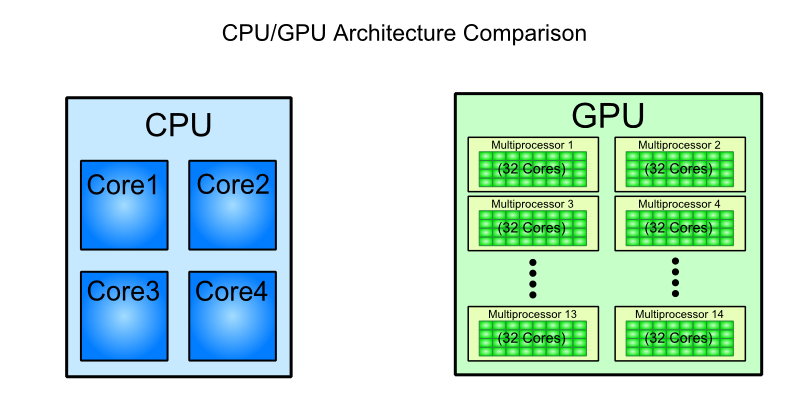
\includegraphics[width=0.75\textwidth,keepaspectratio=true]{images/cpu_vs_gpu.png}
  \caption{Multicore CPU's and Manycore GPU's have fundamentally different design philosophies}
  \label{fig:CPUvsGPU}
\end{figure}

The real difference between multi-core and many-core computing can be seen in Figure ~\ref{fig:CPUvsGPU}, whereby a multi-core CPU, such as the Intel Core i5, has a number of large distinct Processing Units (PUs\nomenclature{PU}{Processing Unit}), whereas an NVidia GPU\footnote{Used as an example of Many-core computing; the general principals apply across many-core devices} consists of an array of many smaller Streaming Multiprocessors (SM) that themselves contain an array of Streaming Processors (SP\nomenclature{SP}{Streaming Processor})\footnote{These principals will be covered in more detail in Section ~\ref{sec:GPGPU}}, each of which can be considered an individual PU.

While it is not directly relevant to this document, outside of the semiconductor industry, the drive towards massively distributed clusters of not-necessarily-co-located machines \footnote{Made famous by SETI@Home in 1999} has become such a major feature of the scientific computing landscape, that it is currently being used at CERN. Data processing for CERN's LHC project is handled by a worldwide grid of over 200,000 processing cores, with 150 PB of storage, and a theoretical capacity to handle the 27TB of raw data per day coming out of the LHC. This grid system is inter-connect agnostic, communicating across a mixture of dedicated fibre connections and the public internet backbone. On a smaller scale, programming paradigms such as Message Passing, and Parallel Virtual Machines, allow applications to be executed against an arbitrary number of computing nodes in a local or distributed cluster.

Before looking back at GPGPU and Parallel Programming in detail, it is important to establish the 'families' of parallelism; namely 'Flynn's Taxonomy'

\subsection{Forms Of Parallelism, aka, Flynn's Taxonomy}
Based on the interactions between instructions and data, Flynn \cite{Fly72} classified computation systems in terms of how Processing Units (PU)\footnote{Think of cores or threads of execution} process instructions and data.

\begin{figure}[H]
  \centering
  \subfloat[SISD]{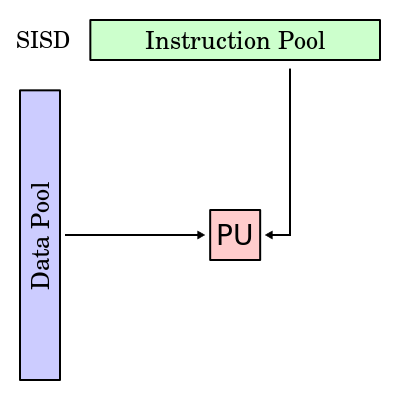
\includegraphics[width=0.25\textwidth,keepaspectratio=true]{images/SISD.png}}
  \subfloat[SIMD]{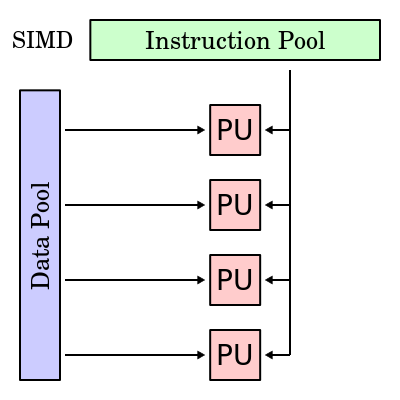
\includegraphics[width=0.25\textwidth,keepaspectratio=true]{images/SIMD.png}}
  \\
  \subfloat[MISD]{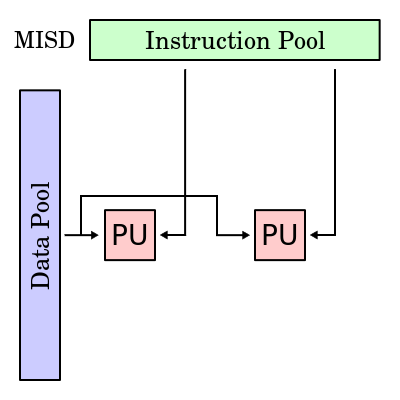
\includegraphics[width=0.25\textwidth,keepaspectratio=true]{images/MISD.png}}
  \subfloat[MIMD]{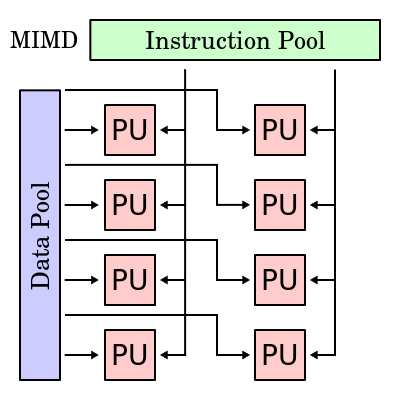
\includegraphics[width=0.25\textwidth,keepaspectratio=true]{images/MIMD.png}}
  \caption{Flynn's Taxonomy of Parallel Computing Systems}
  \label{fig:FlynnsTaxonomy}
\end{figure}

\begin{figure}[h!]
  \begin{minipage}{\textwidth}
\begin{tabularx}{\textwidth}{|c|p{7.5cm}|X|}
  \hline
  Class&Description&Example\\ \hline
  SISD&Single Instruction, Single Data Stream&Traditional Serial Processing\nomenclature{SISD}{Single Instruction, Single Data Stream}\\
  SIMD&Single Instruction, Multiple Data Stream&GPGPU\footnote{Not really any more, but we're getting to that}/Many-core\nomenclature{SIMD}{Single Instruction, Multiple Data Stream}\\
  MISD&Multiple Instruction, Single Data Stream&(Rare\footnote{This architecture is generally only applied where redundancy is critical, and the 'Multiple Instructions' operate on the signal data stream and must agree. One prominent example is the Space Shuttle Flight Control systems})\nomenclature{MISD}{Multiple Instruction, Single Data Stream}\\
  MIMD&Multiple Instruction, Multiple Data Stream&Cluster/Grid systems (e.g. LHCGrid)\nomenclature{MIMD}{Multiple Instruction, Multiple Data Stream}\\
  \hline
\end{tabularx}\caption{Flynn's Taxonomy of Parallel Computation}\label{tab:flynn}
\end{minipage}
\end{figure}

Intuitively, this breakdown is a matrix of data and instruction parallelism. Taking SISD and SIMD separately (as they are the most familiar and relevant), SISD performs a single operation on a single piece of data. It can only process that one piece of data at a time, and can only execute one instruction at a time\footnote{Don't worry dear readers, pipe-lining is coming...}. SIMD on the other hand takes that one execution instruction, and can operate on many pieces of data, producing many results in parallel. This behaviour is augmented in MIMD, where data and instructions are processed in parallel; this could be within a single device (Such as the Cell Broadband Engine) or distributed across the globe.

Flynn created a very clear and simple map of parallelism. Unfortunately the real world got in the way and complicated things. Two major 'complications' will be addressed that have muddied the taxonomic water; SISD Instruction Pipe-lining, and Single Program Multiple Data (SPMD\nomenclature{SPMD}{Single Program Multiple Data Stream}) execution.

\subsubsection{Pipe-lining}
Computer processors are not monolithic boxes that have data pumped into them and the results instantly come out; within even a basic microprocessor, there are a variety of hardware sections that work in sequence, making data and instructions flow through the device to produce the correct result. This sequence is termed the 'pipeline'.

A Generic pipeline consists of four steps;
\begin{enumerate}
  \item Fetch
  \item Decode
  \item Execute
  \item Write-back
\end{enumerate}

Simply put, Fetch grabs the next instruction to be executed from local memory, Decode processes that instruction, prepares the processor's Arithmetic Logic Unit (ALU) for execution, as well as establishing appropriate data I/O memory channels. During Execute, the calculation is performed, and during Write-back, the result of the calculation is stored back in memory. For the sake of simplicity it can be assumed that each of these stages takes one clock cycle.
These tasks are performed by different areas of the chip. This opens up the possibility of having multiple instruction pipelines 'running' at once; 

\begin{figure}[h!]
  \centering
  \subfloat{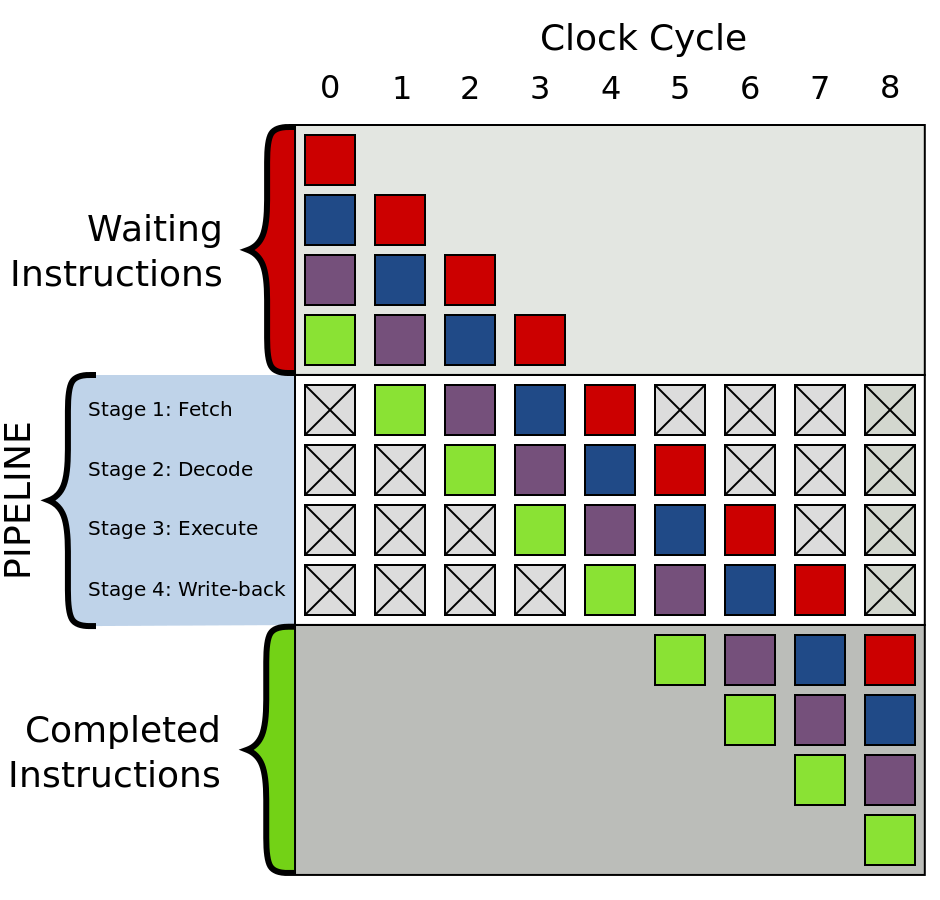
\includegraphics[width=0.4\textwidth,keepaspectratio=true]{images/Pipeline.png}}
  \caption{Example of a 4 Stage Pipeline system}
  \label{fig:Pipeline}
\end{figure}

Looking back to Flynn's Taxonomy, it appears at first glance that what was previously a solid SISD processor could be considered MIMD; the data fetched can be different for each pipelined instruction, and those instructions do not have to be the same either. Whether this counts as true parallelism or not is not as important as its performance improvement; where previously one instruction took four clock cycles to execute, with this simple four stage pipeline, four instructions can be processed in 8 clock cycles.\footnote{Complications to this system arise if the instructions processed are conditional, but as pipe-lining is not the focus of this project, refer to \cite{Yeh91} for more information}

\subsubsection{Single Program Multiple Data}
SISD implementations, at least as developed when Flynn stated his Taxonomy, meant that each machine-level instruction was executed in parallel in lock-step. This meant that data-dependent conditional execution simply wasn't possible without suspending the operation of PUs for which that condition was not satisfied.
SPMD is a subset of MIMD whereby each PU can continue on at its own execution pace, regardless of the state of other PUs. This is exemplified in the Message Passing Interface (MPI\nomenclature{MPI}{Message Passing Interface}) model, where by a (usually) identical program is executed by all PUs, and to control collective program flow and distribution of data, messages are send and received asynchronously between PUs. These PUs could be processor cores within a single machine, or indeed on the same, multi-threading, core, or they could be on machines on opposite sides of the globe.
To add more confusion, in the strictest sense, GPU execution (at least under CUDA) is another different form of parallelism; Single Instruction Multiple Thread (SIMT\nomenclature{SIMT}{Single Instruction Multiple Thread Stream}), which can be though of as a blend of SPMD and SIMD, whereby execution is done is collections of threads simultaneously, and within these collections, instructions are carried out in lock-step as in SIMD, but these collections can be swapped in and out from execution for a variety of reasons, and reorganised based on run-time decisions and resource requirements. The subtleties of this will be discussed in Section ~\ref{fig:CUDAExecArch}.

\subsection{Principles of Parallel Programming}
The concept of splitting a problem set up for separate execution is intuitively simple but in practise very difficult, and has been the major stumbling block in terms of widespread adoption of the parallel programming paradigm. But the potential performance gains afforded from even rudimentary parallelism can be astounding when applied to real world problems.

Examples of problems that are inherently parallel can be found all over the natural and mathematical world; Climate systems can be modelled as atmospheric cells that respond to changes in their surroundings, as can Computational Fluid Dynamics (CFD) and particle physics; Image processing, such as real time video compression can enjoy massive gains as sectors of a video stream can be isolated and processed independently; Linear Algebra, and anywhere where linear algebra is applied\footnote{It's everywhere} is extremely parallelisable in higher-order matrices.

\subsubsection{Gustafson and Amdahl's laws}
Performance improvements from parallelism are not perfect however, as any problem will still retain some operations that are inherently serial.

This limitation has been codified by Gene Amdahl in the law that takes his name\cite{Amd67}, which states that this serial portion of the problem, however small, will limit the overall speed-up provided from parallising the problem. This is stated mathematically in equation ~\eqref{fig:AmdahlsLaw}, where \(\alpha\)\nomenclature{\(\alpha\)}{Fraction of an application that cannot be parallelised} represents the fraction of the program that cannot be parallelised, and graphically in Figure ~\ref{fig:AmdahlFigure}. It is colloquially phrased as:

\begin{quotation}
When a task cannot be partitioned because of sequential constraints, the application of more effort has no effect on the schedule; The bearing of a child takes nine months, no matter how many woman are assigned
\end{quotation}

\begin{equation}
\label{fig:AmdahlsLaw}
S=\frac{1}{\alpha}
\end{equation}

\begin{figure}[h!]
  \centering
  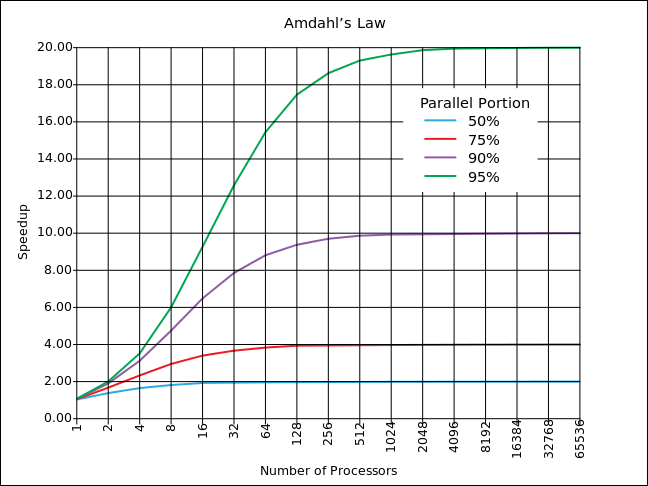
\includegraphics[width=0.75\textwidth,keepaspectratio=true]{images/AmdahlsLaw.png}
  \caption{Graph demonstrating the maximum speed-up attained with a variety of parallelisable program ratios under Amdahl's Law}
  \label{fig:AmdahlFigure}
\end{figure}


Amdahl's Law assumes that the execution time of the non-parallelisable section of the problem is independent of the number of processors available to the system, and that the problem size is fixed. Gustafson's Law\cite{JLG88} at least partially contradicts Amdahl's Law, by stating that for problems with large datasets, parallelisation is still a worthwhile pursuit, regardless of the sequential portion; effectively implying that while parallelism can't make such problems 'faster', the size of their tractable problem sets can be increased if the serial section does not 'slow down' with the problem set size increasing. This is stated mathematically in ~\eqref{fig:GustafsonsLaw} , where \(P\) is the number of processing units available, and graphically in Figure ~\ref{fig:GustafsonFigure}.

\begin{equation}\label{fig:GustafsonsLaw}
S(P)=P-\alpha(P-1)
\end{equation}

\begin{figure}[h!]
  \centering
  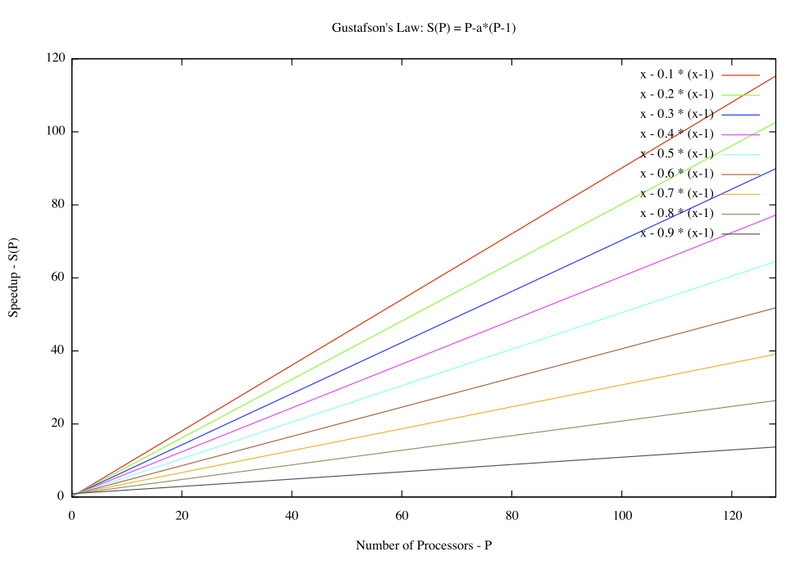
\includegraphics[width=0.\textwidth,keepaspectratio=true]{images/GustafsonsLaw.png}
  \caption{Graph demonstrating the maximum speed-up attained with a variety of parallelisable program ratios under Gustafson's Law}
  \label{fig:GustafsonFigure}
\end{figure}

The both of these Laws are purely theoretical, and do not include aspects of computation such as communication time between PUs, Memory constraints leading to cache contention\footnote{Whereby working data is partitioned across PUs, and in order to maintain the integrity of these caches with respect to the global data state, additional processing is required} or simple processing over-heads involved in running multiple PUs. As such, these Laws can only act as an upper limit to the possible performance of Parallel systems.

\subsection{General Purpose computing on Graphics Processing Units}
\label{sec:GPGPU}
Graphics Processing Units were specialised co-processors designed for real-time image processing and generation, with a focus on the fast growing video game industry. The general architecture of GPU's was designed to perform massive numbers of floating point calculations on each video frame, simulating lighting, texturing, and collision detection events for display devices. This led to quite unique design practices in terms of memory management and execution structures. To put this in perspective, main memory access bandwidth from a High End CPU currently stands at approximately 50GB/s\cite{Var11}, a third of the bandwidth of a similar-generation GPU\cite{NC10}. The idea being that graphics textures are being read many many times over by the collection of PUs, and so needs to be fast.

Around the late 1990's, as this type of hardware became very common on even private desktop machines, the scientific computing community began to use these devices for accelerating highly complex simulations and problems. Up until 2007, in order to accomplish this, the scientific computing problem would have to be 'rephrased' into a graphical problem, utilising a graphics API\footnote{Application Programming Interface\nomenclature{API}{Application Programming Interface}: DirectX and OpenGL allowed game developers to have a hardware-agnostic interface to leverage GPUs and other hardware} such as DirectX or OpenGL. This meant that problems such as matrix multiplication had to be rephrased as overlays of transparent textures, as a contrived example. Taking larger more abstract computational problems and decomposing them into graphical operations was far from simple, and was a major block for many institutions with a desire to use these highly parallel devices.

In 2007, NVIDIA released a new reference architecture for its high-end graphics cards, specifically aimed at the scientific and application-acceleration communities; the Compute Unified Device Architecture (CUDA)\cite{NC07}. CUDA was not just a new C/C++/FORTRAN API, exposing low-level execution and memory control to scientific computing, but was a complete re-write of all intermediate software layers, and included the addition of specific interface hardware, along side the standard graphics interface, dedicated for CUDA computing\cite{DBK10}, see Figure ~\ref{fig:CUDAArch}. In 2007, one GPU chip-set supported CUDA; the G80. In 2008, The Tokyo Institute of Technology's TSUBAME supercomputer became the first GPU accelerated machine in the Top500 World Supercomputer rankings\footnote{TSUBAME made it to 29th in the world rankings, with the addition of 170 Tesla S1070 systems\cite{Hum08}}. By 2011, over 20 different chipsets encompassing over 40 individual manufacturer cards and hundreds of after-market cards, constituting over 100 million CUDA-enabled cards\cite{iVE10} sold across the globe.

In 2008, Apple Inc, in collaboration with NVidia, Intel, IBM and AMD released a C/C++ based framework for mixed CPU/GPU/Manycore/FPGA heterogeneous computing called OpenCL (Open Computing Language). OpenCL contains much more programming abstraction away from the hardware compared to pure-CUDA, and as such cannot be as highly optimised. Even still, NVidia rolled out agnostic device interfaces to OpenCL. The current CUDA architecture is shown in Figure ~\ref{fig:CUDAArch}

\begin{figure}[h!]
\centering
  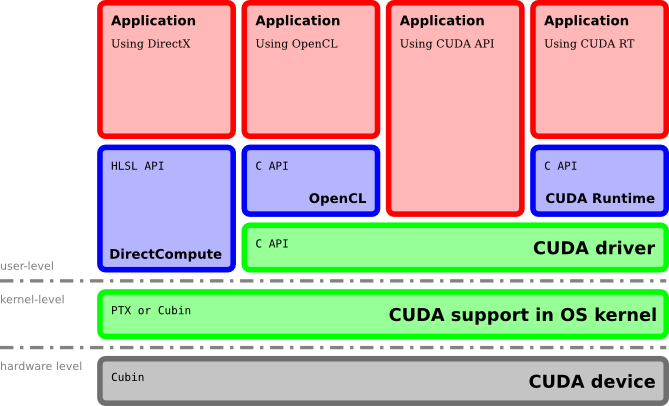
\includegraphics[width=0.75\textwidth,keepaspectratio=true]{images/cuda_architecture.png}
  \caption{Diagram showing levels of abstraction between Hardware and various APIs}
  \label{fig:CUDAArch}
\end{figure}

\subsection{CUDA Execution architecture}\label{fig:CUDAExecArch}
A CUDA execution consists of both host (CPU) and device (GPU) phases. The device phases, called kernels, are written in C/C++\footnote{As we'll see, wrappers for other languages exist, but there is always an intermediate C/C++ stage}. Since these kernels reside only on the device, access to main host memory is impossible, and data sets to be worked on, as well as areas of memory to store results, must be set-up by the host on the device before invocation. The amount of parallelism used by the kernel is decided per-kernel invocation, but the kernels themselves must be written with this level of parallelism in mind; there are no magic tricks in CUDA. To understand this, the low level architecture of the GPU must be investigated. 

\begin{figure}[h!]
  \centering
  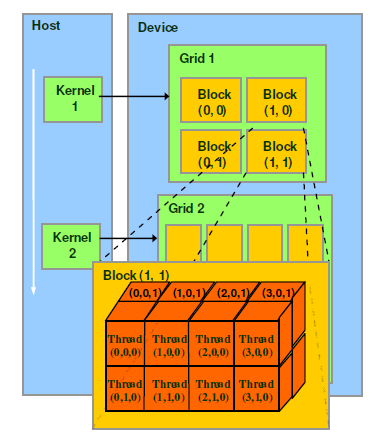
\includegraphics[width=0.45\textwidth,keepaspectratio=true]{images/CUDA_host_dev_threads.png}
  \caption{Diagram showing levels of execution between host and CUDA device operations}
  \label{fig:CUDAHostDevExec}
\end{figure}

Starting from the top down, a host machine can have multiple GPU devices, which can all be individually addressed for asynchronous execution in parallel. Below this level, and as shown in Figure ~\ref{fig:CUDAHostDevExec}, there are logical 'Grids', which contain logical 'Blocks' of threads. These Grids and Blocks are the fundamental form of execution parallelism. As shown in Figure ~\ref{fig:CUDAHostDevExec}, Grids can be thought of as two dimensional arrays of Blocks, and Blocks are thought of as three dimensional arrays of Threads. It is these threads that actually execute any particular workload.

\begin{figure}[!h]
  \centering
    \begin{lstlisting}[numbers=left, language=C, numberstyle=\tiny, numbersep=8pt]
    //Setup dimensions of grids and blocks
    dim3 blocksPerGrid(65535,1,1);
    dim3 threadsPerBlock(64,8,1);

    //Invoke Kernel
    kernelfunction<<<blocksPerGrid,threadsPerBlock>>>(*functionarguments);
    \end{lstlisting}
  \caption{Example CUDA host code segment, showing kernel invocation}
  \label{fig:KernelInvocation}
\end{figure}

As stated, the level of parallelism is defined at the kernel invocation stage and (until very recently\footnote{The latest Fermi devices support multiple parallel kernel invocations, under which SMs are assigned different kernels based on a proprietary load-balancing algorithm}) only one kernel can run on a single device at a time. Following the SIMD model, parallelism is attained by per-thread self-indexing. In the case of CUDA, each thread could generate a unique 1D execution index using a combination of runtime variables that are pro grammatically exposed through the CUDA Driver API, as shown in Figure ~\ref{fig:GridBlockThread1D}. In this particular example, it assumed that both Grid and Block dimensions are 1D. This is useful in this case for scalar multiplication of linear arrays, and could process input data containing \(2^{16}\times 2^{10} = 2^{27}\), or over 67 million values\footnote{For the latest generation of Tesla GPUs}. CUDA introduces several additional keywords to the C language, in this case "\_\_global\_\_", which indicates that the function is executed on the device, but can be called from the host. A summary of these function declaration keywords is shown in Table ~\ref{tab:CUDAFuncDecTable}

\begin{figure}[!h]
  \centering
    \begin{lstlisting}[numbers=left, language=C, numberstyle=\tiny, numbersep=8pt]
    __global__ void multArray(float *array, float multiplier){
      int 1Dindex = blockIdx.x*blockDim.x+threadIdx.x;
      array[1Dindex]=array[1Dindex]*multiplier;
    }
    \end{lstlisting}
  \caption{Example CUDA kernel, showing 1D index identification}
  \label{fig:GridBlockThread1D}
\end{figure}


\begin{table}[!ht]
\begin{tabularx}{\textwidth}{|X|c|c|}
Function Declaration&Executed by&Callable From\\\hline
\_\_device\_\_ void someKernel&device&device\\
\_\_global\_\_ void someKernel&device&host\\
\_\_host\_\_ void someKernel&host&host\\
\end{tabularx}
\caption{Table of CUDA Function Declaration Keywords and their use}\label{tab:CUDAFuncDecTable}
\end{table}

For more parallelism, and more context relevance, consider scalar multiplication of large matrices. The previously stated indexing scheme could be used sequentially, i.e taking each row of the matrix in turn and farming the computation of that row to the GPU, but as stated, CUDA allows (actually encourages) multi-dimensional indexing, so each thread execution could be tasked with modifying multiplying one matrix element by 2D addressing, as shown in Figure ~\ref{fig:GridBlockThread2D}. This form of parallelism theoretically allows for up to \(2^{16}*2^{16}*2^{10}*2^{10}=2^{52}\) or about 4.5 quadrillion threads, (i.e operating on a square matrix of side \(2^{27}\))\footnote{Due to Memory and Hardware considerations, this is a ridiculously contrived metric}.

\begin{figure}[!h]
  \centering
    \begin{lstlisting}[numbers=left, language=C, numberstyle=\tiny, numbersep=8pt]
    __global__ void multMatrix(float *matrix, float multiplier){
      int x_index = blockIdx.x*blockDim.x+threadIdx.x*;
      int y_index = blockIdx.y*blockDim.y+threadIdx.y*;
      matrix[x_index][y_index]=matrix[x_index][y_index]*multiplier;
    }
    \end{lstlisting}
  \caption{Example CUDA kernel, showing 2D index identification}
  \label{fig:GridBlockThread2D}
\end{figure}

Moving into the practical realm, once a kernel is launched, the CUDA runtime system generates the corresponding logical grid of threads. These threads are assigned to execution resources such as shared memories and thread registers\footnote{These will be covered in detail in Section ~\ref{fig:CUDAMemArch}} on a block-by-block basis\footnote{For the sake of simplicity, the following section discusses the hardware capabilities of the latest generation of Fermi cards, specifically the Tesla C2050 Workstation card}. These resources are organised into streaming multiprocessors (SMs), the number of which vary depending on the particular hardware, but usually around 15 are active. These SMs can each be assigned up to 32 thread-blocks, each of which is executed on a separate Streaming Processor (SP) core. These cores can handle up to 48 threads in parallel. In the case of the Tesla C2050, this means that over 20,000 threads can be 'simultaneously' executed.

Note that this does not limit the grid and block dimensions; groups of threads, termed warps, are swapped in and out of the SM's regularly, making execution tolerant of long-latency operations such as global memory access. This warping of threads is also an important concept for thread-divergence; when runtime-dependant conditional statements in kernel execution have different branching behaviours in threads that are in the same 'warp', the warp is actually executed twice; once for the major condition, and once for the minor condition. Between these two executions, the results obtained from the 'minor' path are discarded and during the minor execution, the results from the major path are also discarded. It is for this reason that conditional behaviour should be avoided in a GPU environment (Figure ~\ref{fig:thread-divergence} demonstrates this. Adapted from \cite{KF08}). 

\begin{figure}[h!]
  \centering
  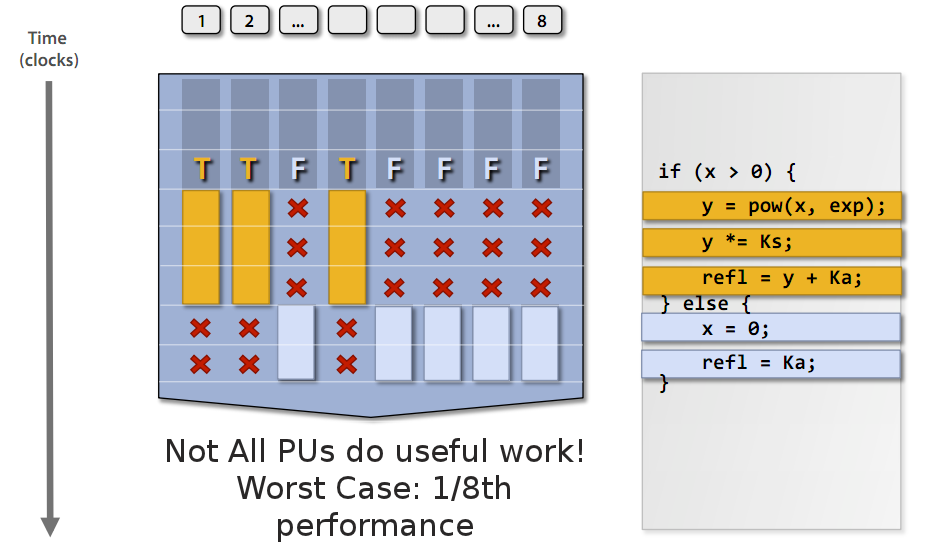
\includegraphics[width=0.75\textwidth,keepaspectratio=true]{images/thread_divergence.png}
  \caption{Diagram showing thread divergence operation under CUDA, adapted from SIGGRAPH 2008 proceedings}
  \label{fig:thread-divergence}
\end{figure}

As mentioned, resource allocation is partially decided upon the memory requirements of a particular kernel. These and other memory related concepts are covered in the following section.

\subsection{CUDA Memory architecture}
Utilising the levels of parallelism demonstrated previously, one would expect massive performance improvements to be a given. This is not the case, and 'lazily parallelised' applications generally achieve only a small fraction of the potential speed of the underlying hardware, and most of the time, the limiting factor is memory latency. To understand why this is the case, it is important to investigate the CUDA memory architecture.

CUDA devices have three major levels of memory; Thread local, Block Shared, or Grid Global. This architecture is displayed diagrammatically in Figure ~\ref{fig:CUDAMemArch}, and summarised in Table ~\ref{tab:CUDAMemTable}.

\begin{figure}[h!]
  \centering
  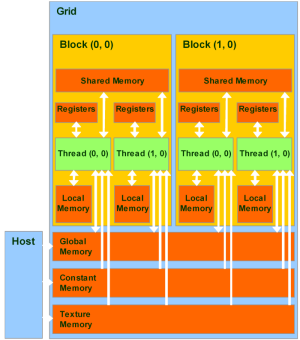
\includegraphics[width=0.5\textwidth,keepaspectratio=true]{images/cuda_mem_arch.png}
  \caption{Diagram showing CUDA memory access architecture}
  \label{fig:CUDAMemArch}
\end{figure}

\begin{table}[!ht]
\begin{tabularx}{\textwidth}{|c|c|c|c|X|c|}\hline
Memory&Scope&Lifetime&R/W&Usage&Speed\\\hline
Register&Thread&Kernel&R/W&Automatic variables other than arrays&Very Fast\\
Local&Thread&Kernel&R/W&Automatic Array Variables&Very Fast\\\hline
Shared&Block&Kernel&R/W&\_\_shared\_\_&Fast\\\hline
Global&Grid&Application&R/W&Default&Very Slow\\
Constant&Grid&Application&R&\_\_constant\_\_&Slow\\\hline
\end{tabularx}
\caption{Table of CUDA Memories and some characteristics}
\label{tab:CUDAMemTable}
\end{table}

In order to get data to and from the device, Global, Constant and Texture memory is read-write accessible from the host; any other memory allocation is done on a per-thread basis.

Texture memory is a particular area of constantly declared memory that is logically represented as a 2D array, and is augmented with a distributed cache of 2D localised values from last access and as such is significantly faster than Global memory. This behaviour is particularly useful for applications such as linear algebra and CFD.

Due to their scientific ubiquity, parallelisation of linear algebra systems is a heavily researched field, leading to highly customised libraries available, such as BLAS (Basic Linear Algebra Subprograms) and MKL (Math Kernel Library). cuBLAS is a CUDA library specifically optimised for most Level 1, 2, and 3 BLAS functions running on GPU, and this library and others like is is heavily used within the research community\cite{MF08}.

This competitive optimisation in all linear algebra systems means that defined linear algebra functions are a natural benchmark for cross-comparison between parallel CPU and GPU implementations; each candidate library doing the best they can do with the hardware. And frankly, GPU wipes the floor with CPU, as in Figure ~\ref{fig:BLASComp}.

\begin{figure}[h!]
\centering
    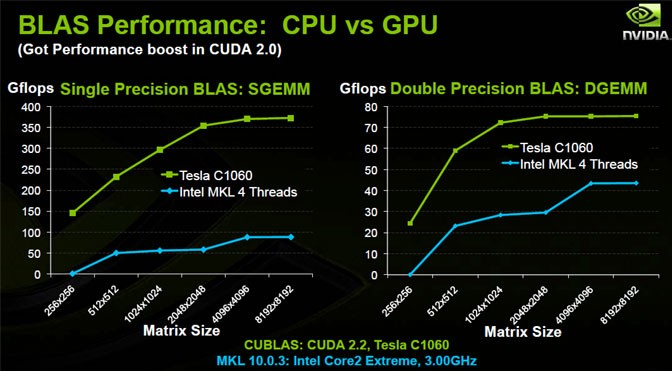
\includegraphics[width=0.75\textwidth,keepaspectratio=true]{images/NVDA_BLAS_C1060_vs_CPU_675.png}
  \caption{Image Courtesy of NVidia Corp. Showing CPU/GPU comparison of highly optimised BLAS libraries}
  \label{fig:BLASComp}
\end{figure}

In \cite{DBK10}, a variety of matrix multiplication kernels designed for matrices of many thousands of elements are shown with a variety of optimisations. A Naive implementation is shown, as in Figure ~\ref{fig:MatMulNaive} that performs at (only) 17.2 GFLOPS\footnote{Giga-Floating Point Operations per Second}. With a few modifications, a similar kernel (Figure ~\ref{fig:MatMulShare}) can perform at 47.5 GFLOPS; nearly 280\% faster. The major modification is the use of what is called 'shared' memory, i.e memory that is common to a thread-block.

In Figure ~\ref{fig:MatMulNaive}; matrix pointers \(A, B, C\) point to the two input and one output matrix respectively, where global memory has been allocated and moved onto the device by the host application, and the kernel is invoked with the width of the matrix to stay in memory bounds. Each block of threads will calculate a section of the output matrix, as shown in Figure ~\ref{fig:MatMulNaiveDiag}.

\begin{figure}[!h]
  \centering
    \begin{lstlisting}[numbers=left, language=C, numberstyle=\tiny, numbersep=8pt]
      __global__ void matmulNaive(float *A, float *B, float *C, int WIDTH){
        Tx = threadIdx.x; Ty = threadIdx.y;
        Bx = blockIdx.x; By = blockIdx.y;

        X = Bx * blockDim.x + Tx;
        Y = By * blockDim.y + Ty;

        idxA = Y * WIDTH;   
        idxB = X;
        idxC = Y * WIDTH + X;

        Csub = 0.0;

        for (i=0; I < WIDTH; i++) {
          Csub += A[idxA] * B[idxB];
          idxA += 1;
          idxB += WIDTH;
        }

        C[idxC] = Csub;
      }
    \end{lstlisting}
  \caption{Example CUDA kernel, showing Naive parallel matrix multiplication with Global memory access}
  \label{fig:MatMulNaive}
\end{figure}

\begin{figure}[h!]
\centering
  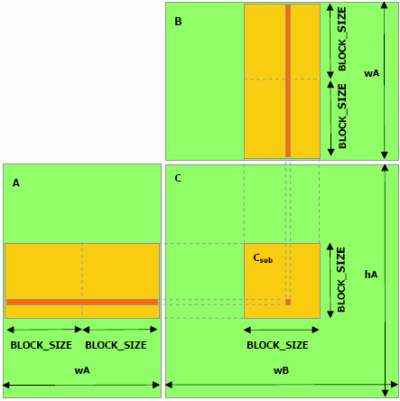
\includegraphics[width=0.45\textwidth,keepaspectratio=true]{images/naive_matrix.png}
  \caption{Naive matrix calculation with memory access by a single block highlighted}
  \label{fig:MatMulNaiveDiag}
\end{figure}

In this example, every access to A, B, or C (lines 15 and 20) is from/to Global memory. This access is orders of magnitude slower than the access to thread-local variables such as the A and B indexes. One improvement that can be made initially is to use block-shared memory. This is demonstrated in Figure ~\ref{fig:MatMulShare}. In this case, each thread retrieves one element from each input array, and stores it in block-shared memory, i.e the threads collaboratively copy the data required for whole-block execution. Note the \_\_syncthreads() in lines 19 and 22; this CUDA call instructs each thread in the block to wait for all other threads in the block to come to the same execution point before continuing. In this case this is to ensure that all of the relevant elements have been copied by all of the block-warps before trying to do any actual calculations. The operation is similar to previous, as shown in Figure ~\ref{fig:MatMulNaiveDiag}, except that the outer while loop makes each thread 'step' across the input matrices. This has the effect of greatly reducing the number of Global memory accesses, and has the added benefit of increasing what is called coalesced memory access.

\begin{figure}[!h]
  \centering
    \begin{lstlisting}[numbers=left, language=C, numberstyle=\tiny, numbersep=8pt]

        __shared__ float As[blockDim.x][blockDim.y];
        __shared__ float Bs[blockDim.y][blockDim.x];
        Csub = 0.0;
        Tx = threadIdx.x; Ty = threadIdx.y;
        Bx = blockIdx.x; By = blockIdx.y;

        X = Bx * blockDim.x + Tx;
        Y = By * blockDim.y + Ty;

        idxA = Y * WIDTH;   
        idxB = X;
        idxC = Y * WIDTH + X;

        while (idxA<WIDTH) {  // iterate across tiles
          As[Ty][Tx] = A[idxA];
          Bs[Ty][Tx] = B[idxB];
          idxA += blockDim.x;  idxB += blockDim.y * WIDTH;
          __syncthreads();
          for (i=0; i < 16; i++) {
            Csub += As[Ty][i] * Bs[i][Tx];
            __syncthreads();
          }
        }
        C[idxC] = Csub
    \end{lstlisting}
  \caption{Example CUDA kernel, showing Naive parallel matrix multiplication with Shared memory access}
  \label{fig:MatMulShare}
\end{figure}

Coalesced memory accesses are simply batching of memory reads and writes, where all (or most) threads in a warp access a linearly contiguous data space, i.e the \(k^{th}\) thread in a given warp accesses the \(k^{th}\) element of an array. This way, the 'block' SP can perform these reads or writes as one instruction, instead of each individual thread accessing individually. In this case, matrix A accesses are largely coalesced, as each thread is grabbing its own element within a row of A, but B accesses are uncoalesced. One solution, that will not be investigated here, is performing an transpose on B and then performing the more complex multiplication; this operation would only be useful for fairly large Matrices.

Looking beyond shared memory and memory coalescing schemes schemes, CUDA exposes many memory access interfaces for handling different arrangements of data, and for more detailed information refer to \cite{NC11}.

In summary, the performance of CUDA, and generally any, parallel application is dependant on many factors; from efficient runtime resource allocation; memory types and access techniques; and most importantly, input data dimensions. This is demonstrated when matrix multiplication algorithms are used applied to 'smaller' matrices; Figure ~\ref{fig:CPU_GPU_MATMUL_SMALL} shows that for small matrices, \(N~180\), CPU-bound calculation is significantly more performant than GPU-bound solutions. From this section it is clear why this is so; memory latency, kernel processing overheads, and a minimal workload all work against a parallelised GPU implementation. Where the problem set is large, for instance, warp-swapping is used to continue to efficiently provision resources to queued warps while other warps are waiting on memory retrievals.
This economy of scale is an important design heuristic when developing for GPU and will significantly influence the allocation of work in this project.

\begin{figure}[h!]
\centering
    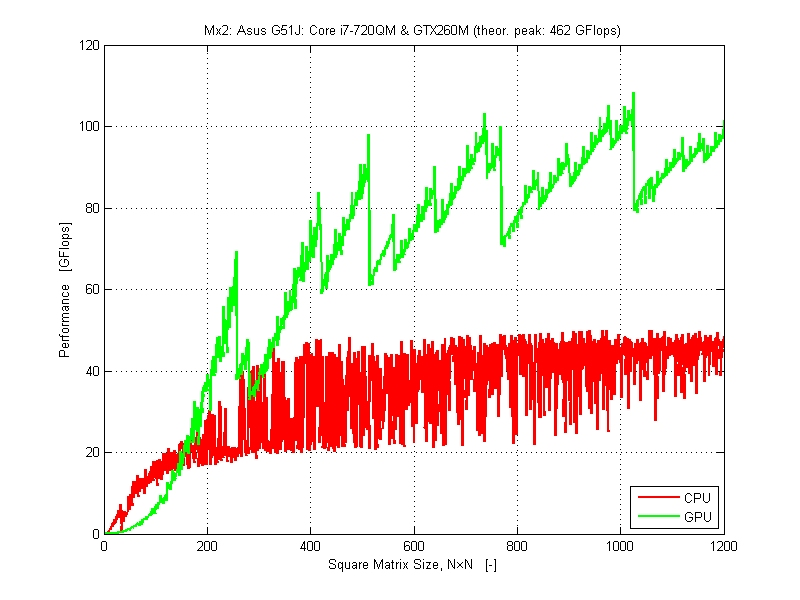
\includegraphics[width=0.75\textwidth,keepaspectratio=true]{images/FlopsMx2_Asus_G51J_02.png}
  \caption{Image Courtesy of AccelerEyes  Showing lower order CPU/GPU comparison of MATLAB Matrix Multiplication using the Jacket framework}
  \label{fig:CPU_GPU_MATMUL_SMALL}
\end{figure}

\section{Opportunities for Parallel Decomposition of DSM Algorithms}
With an understanding of the mathematical challenges presented in the DSM problem, and the current availability of Parallel Computing technologies (specifically those presented by innovations in GPGPU), it is worthwhile to pause and analyse potential decomposition techniques that could be applied to algorithmic acceleration.

In \cite{AM09}, McKinley observes that the majority of computational time accrued in the generation of optimal and near-optimal bit-loading configurations is in the calculation of power spectral densities of candidate bit-loads. This naturally stems from the previously discussed exponential relationship between number of lines, maximum bits-per-tone, and the resultant number of possible bit-combinations. The calculation of PSDs is the solution of \(N\) linear systems, as stated in equation ~\eqref{eq:SysModMat}.

As discussed in Section ~\ref{sec:ParallelComputing}, parallel computation is ideal, especially under the CUDA model, for solving systems of linear equations with high \(N\). The downside is that to utilise parallelism effectively, the number of systems must be quite large (100+, see Figure ~\ref{fig:CPU_GPU_MATMUL_SMALL}). Since in general DSM bundles consist of 50 lines, and range up to 100, there is no rational justification for offloading this work to existing libraries such as cuBLAS, as they will perform significantly worse than equally optimised CPU-bound libraries.

Even so, the small \(N\) also can be an advantage; considering the previously discussed memory architecture of CUDA, it is feasible to create a small, customised, linear system solver that resides in-thread; i.e, each thread solving one small system of equations. 

To restate the DSM problem in general; the process of generating optimal bit-load configurations is a \(N\) dimensional optimisation problem, and as such stands as one of the most difficult problems in computation, which has not completely been 'solved' in either the sequential or parallel realms \cite{JDJZW03}.

This allows a simplified reclassification of the previously discussed DSM algorithms in terms of purely their qualitative searching techniques; OSB exhibits \(N\) dimensional exhaustive search behaviour, ISB exhibits behaviour similar to segmented linear search schemes, and MIPB takes a heuristic increment-and-search approach. 

The range of these behaviours immediately indicates that no 'one-size-fits-all' solution is going to work; each problem will have to be tackled individually.

\subsection{Parallel OSB}
Even though OSB is a computationally explosive searching solution, it would still be worth while to attempt to parallelise it, as it is the 'simplest' of algorithms, and its core can be explained quite simply; For each channel, calculate the PSD's of every possible bit-loading combination, subsequently find the Lagrangian cost for this bit-load scheme on this channel, and thus return the maximally optimal bit-loading combination for the entire bundle on this channel. 

It's clear even from this simple statement that parallelisation will be effective; Each thread can calculate the PSD and subsequent Lagrangian for each bit-combination in parallel, then a reduction can be used to find the maximum Lagrangian and bit-load. This presents a prarallelisation across Channels, Lines, and bit-permutations, and would be relatively simple to leverage multiple devices in this scheme; each device is assigned a channel range or a channel queue, and calculates the local optimisation for the channel, returning its result back to the host.

Intuitively, this should give significant speed-up's for lower numbers of lines (i.e up to 4 or 6), but due to bit-combination-explosion, will remain intractable for higher line counts.

\subsection{Parallel ISB}
ISB segments the search problem of OSB such that instead of searching every possible bit-loading combination for every line, per-user bit-loading is searched on each tone, so that in the lowest level, there are \(O(N^2)\) combinations as opposed to OSB's \(O(2^N)\). After searching a single line, the global bit-load for that line is updated, and the next line is searched. 

From a parallelisation perspective, this global updating of bit-loads is concerning as it creates much more opportunity for memory contingency problems as well as non-optimal SM occupancy where the number of users is relatively small (i.e. below 8), as each line-search will have to wait on the search for the previous line. That said that larger numbers of lines, the problem should be highly scalable by having thread blocks collaboratively searching individual line loads and continuously updating a global record of bit-loads. Indeed there is the possibility of having larger thread blocks that individually search different lambda values in parallel, simplifying bisection search. Another possibility is to invert the ISB looping constructs such that all channels can take one 'step' in parallel.

As such, one would hope for at least channel and bit permutation parallelism, but due to the incremental update nature of ISB, could not exhibit line parallelism. This represents a much smaller parallelisation problem which will be significantly more difficult to shoehorn into a multi-device structure due to data dependency, but one would predict that the combination of reduced computational complexity of ISB, and this style of parallelism, that GPU ISB will be very very fast compared to even GPU OSB.

\subsection{Parallel MIPB}
Due to the sequentially coupled nature of the MIPB algorithm, it is inherently difficult to parallelise effectively. MIPB only needs to update one \(N\) psd vector at each bit-increment, and this could only really be accelerated across \(N\) threads. This factor alone indicates that MIPB may not be directly parallelisable in its simple form, but some future adaptations of MIPB utilising the deterministic nature of 'bit-increment chains' presents an algorithmic possibility of pre-computing the bit-increment paths on each channel and using these weighted increment trees to allocate bit-loads based on power constraints.

In any case, MIPB will be implemented as a CPU bound comparison, with an attempt at a GPU implementation, to assess the comparative merits of for instance GPU ISB/OSB against MIPB.


\chapter{Development and Solution}
\label{sec:solution}

After performing research into the problem we now have a better understanding of exactly what needs to be done, and some of the theoretical and implementation based conditions that must be adhered to. It is clear that current implementations of DSM algorithms cannot be put to practical use due to computational intractability with standard sequential hardware, and that a move towards parallelisation has significant potential benefits. But in order to approach the algorithmic problem, first a DSL simulation framework must be created within which to experiment, and this is no small undertaking.

To start with, a stable software base must be selected, that incorporates rapid development due to the expansive scale of this project without sacrificing too much in the way of performance, as well as interoperability with the CUDA API, and is supported by a strong community that can be leveraged to ensure that development is not halted by 'silly' problems.

In \cite{AM09}, McKinley had the same task on his hands, and due to its close-to-the-hardware speed, selected the C programming language. While this was indeed a very fast \footnote{Technically record breaking}, C can often be prohibitively obtuse, with many arcane design patterns and structures that do not aid in rapid prototyping. 

Instead, the Python programming language was selected (in agreement with Dr McKinley) as the base of this project. Python is an interpreted, high-level language, originally created by Guido van Rossum in the 1980's. Two of the biggest draws to Python as a general-purpose language are its flexibility\footnote{Python supports Imperative, Object Oriented, Aspect Oriented and Functional Programming constructs interchangeably} and its extension interface; a significant amount of Python's standard module library is built in C/C++, such that these modules are effectively as fast as straight-C implementations. This is of particular importance with the most popular scientific math library in Python, called Numpy, which is entirely C based and operates very close to the metal, including transparent C-variable assignments and other functionality that preserves the speed of C and the higher level functionality of Python. Additionally, the wealth of Python Profiling\footnote{Profiling is the process of recording a software execution and monitoring the performance and runtime of its constituent functions, providing the developer with a 'look under the hood' to establish what areas of code could be optimised to give the maximum performance improvement with minimum wasted time} tools available means that iterative optimisation (at least of the Python section of the framework) would be painless and fast.

So far, it has been established and justified that Python satisfies the first of the conditions for a stable project base; performance rapid development. To satisfy the second, a Python project called PyCUDA should be noted. 

PyCUDA is a complete CUDA API wrapper for Python, incorporating advantages such as automatic device selection and initialisation, dynamic memory management, kernel templating and direct variable passing, Just In Time (JIT) kernel compilation and invocation, and run-time access to device characteristics and status for dynamic block and grid dimensioning. Unfortunately PyCUDA is lacking in some areas, particularly debugging support, Python Profiling integration (i.e CUDA code will have to be profiled and analyses separately from any other functionality), and automatic multiple device allocation.

Considering these together, the Pros of Python + PyCUDA greatly outweigh their disadvantages. That said, the largest disadvantage is the lack of truly automatic multi-device provisioning, and this is not a major obstacle. Consider this scenario; A single CUDA kernel execution outside of PyCUDA\nomenclature{PyCUDA}{CUDA wrapper for the Python programming language} could execute on multiple devices \footnote{This is technically true only for the latest version of CUDA; at time of writing, 4.0 RC2}, for the planned problem complexities and  data structures, host-to-device memory transactions would eat up any added performance incurred from this style of execution. It is much simpler (and most likely faster) to partition the problem space across the number of available devices, and with the flexibility of Python, this is workable with only a few lines of additional code.

Outside of the programming language itself, utilising a free and open source Distributed Revision Control (DRC) called Mercurial allows for tracking changes and activity in the project, as well as serving as an automatic backup system, through a service called BitBucket, which also provides and issue tracker and on-site wiki for development related notes and tasks.

\section{Solution Development Task list}
In order to fully specify the development of a solution, a task list with appropriate milestones was required to monitor progress and maintain framework stability. This was implemented specifically so that experimental development (or branching) could be explored freely in different development areas (to be detailed), while still allocating time for framework and algorithm re-factoring to leverage shared-object functional decomposition. This task-list mirrors the expanded project objectives in Section \ref{sec:overview}, with additional developmental details.

\begin{enumerate*}
  \item Framework Development and Verification of CPU-bound algorithms
  \begin{enumerate*}
    \item Implementation of Object Oriented DSL bundle simulation framework, with software hooks for algorithm interfacing and standardised result and instrumentation storage formatting.
    \item \emph{Verify Channel Matrix generation against known dataset}
    \item Pure-Python implementation of OSB
    \item \emph{Verify OSB bit-loading against known dataset}
    \item Pure-Python implementations of MIPB and ISB
    \item \emph{Verify results against known dataset}
    \item Refactor algorithm object structure to reduce functional duplication
  \end{enumerate*}
  \item Development and Verification of GPU-bound algorithms
  \begin{enumerate*}
    \item Single GPU implementation of OSB
    \item \emph{Verify results against CPU version}
    \item Multi-device development and implementation of OSB
    \item \emph{Verify results against CPU version}
    \item Single GPU implementation of ISB
    \item \emph{Verify results against CPU version}
    \item Refactor algorithm object structure to reduce functional duplication
  \end{enumerate*}
\end{enumerate*}


\section{Simulation Framework Architecture}
\label{sec:arch}
The architecture of the solution will consist of a simulation framework, emulating the gain-characteristics of an arbitrary DSL bundle structure, with software hooks exposed to any algorithms implemented. 

The fundamental datum required for DSM algorithms is a matrix of crosstalk gains between all lines. This matrix must be generated incorporating the physical relationship of different lines to each other, as well as simulating the material characteristics of the lines themselves in order to calculate the direct gains (i.e the 'cross talk gain' between line \(n\) and itself, or the matrix diagonal).

Once generated, this matrix would describe the bundle of lines, and this inherent value led to the decision to develop the Simulation Framework as an Object Oriented model; the bundle object contains line objects that have individual values, such as their line and network termination locations, noise characteristics, computed SNR, preferential line rates, etc... Additional to these values, each line object exposes internal functions that perform operations on 'itself', such as calculating the far end crosstalk experienced by that line on a particular channel, and the RLCG transfer function over its length. 

The bundle object itself defines the system configuration, and is created from a list of line values read from a file; initially it is planned that this file would contain the LN/NT distances of the line, and if required, the desired rate for that line, but the same theory could be applied to allow mixed material bundles, per line noise characteristics, and other pertinent values. The bundle object's main aims are to initially generate the cross-talk matrix, and subsequently act as an abstraction layer between the DSM algorithm and the individual line values; i.e. the bundle keeps internal arrays to store the power and bit ratings for each line for each channel, which can be operated upon by an external algorithm, and subsequently updated by the bundle itself.

The initialisation of the bundle object (i.e. the generation of the cross-talk gain matrix) can be thought of as a triply nested loop of transfer function calculations, and can be summed up in one sentence: On each sub-channel, for each line (the victim) calculate all the inter-line transfer functions between the victim and every line in the bundle (including itself, but that’s slightly different).

Calculating the direct gain (i.e. the transfer function between the line and itself), the line object simply returns its own transfer function across its length. However, for inter-line (FEXT only, in this project) transfer function calculation, the situation is more complex since lines don't necessarily have the same run length and location; there are nine possible combinations of over-lay between two given lines (plus the case where they don't share any length, hence no FEXT). These are detailed in \cite{RB03} and indicated in Figure ~\ref{fig:FEXT-xtalk-gain}, and this structure was the basis for McKinley's work in this area, but an improved, 'case-less' implementation was generated to segment the line lengths into head length (i.e where one line goes further than the other towards the CO end of the bundle), shared length (where both lines occupy the same sector of the bundle), and tail length( where one line goes further towards the CP end). Each length subsequently has a sector insertion loss (transfer function) and these are multiplied to give the final line transfer function which, incorporating a NICC\footnote{NICC is a UK based communications interoperability standards body} FEXT model function, provides the full length gain response between the two lines on a particular channel.

The operation of segmenting these lengths and producing the cumulative transfer function is numerically subtle but conceptually simple, and with the transfer function configured to return 1 for invalid length values (i.e non-positive lengths), the cumulative transfer function product is effectively self selecting which (if any) sector length values to 'ignore' given different theoretical cases. 

Mathematically,the generation of the inter-line transfer function proceeds thus; 

\begin{equation}
  \begin{array}{l}
  L_h=(V_{lt}-X_{lt})\\
  L_s=\text{abs}(\max(V_{lt},X_{lt})-\min(V_{nt},X_{nt}))\\
  L_t=(V_{nt}-X_{nt})\\
  \end{array}
\end{equation}\label{eq:sectorisation}
\begin{equation}
  \text{insertion loss}(L,F)=\left\{
    \begin{array}{l l}
      \text{transfer function}(L,F) & \quad \text{if}\ L>0\\
      1 & \quad \text{if} L\le 0\\
    \end{array} \right.
\end{equation}\label{eq:insertionloss}
\begin{equation}
  \begin{array}{l}
  H_h=\text{insertion loss}(L_h,f_k)\\
  H_s=\text{insertion loss}(L_s,f_k)\\
  H_t=\text{insertion loss}(L_t,f_k)\\
  H_{\text{total}}=(H_h \times H_s \times H_t)\\
  \end{array}\label{eq:transferproduct}
\end{equation}


This is explained diagrammatically in Figure \ref{fig:FEXT-xtalk-gain}, and the source code for this function as used is in Appendix ~\ref{apx:fext-xtalk-gain}.

\begin{figure}[H]
 \centering
 \subfloat[Case 1]{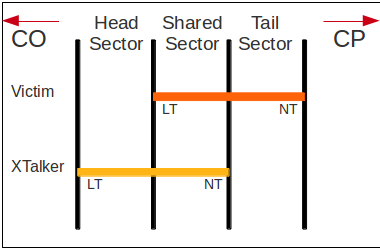
\includegraphics[width=0.35\textwidth,keepaspectratio=true]{images/FEXT_case_1.png}}
 \subfloat[Case 9]{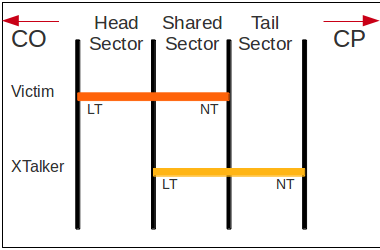
\includegraphics[width=0.35\textwidth,keepaspectratio=true]{images/FEXT_case_9.png}}\\
 \subfloat[Case 2]{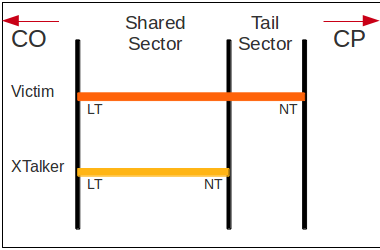
\includegraphics[width=0.35\textwidth,keepaspectratio=true]{images/FEXT_case_2.png}}
 \subfloat[Case 6]{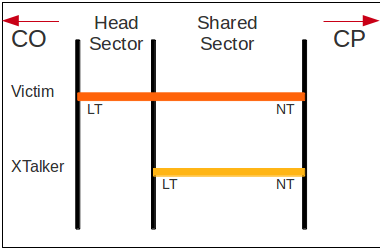
\includegraphics[width=0.35\textwidth,keepaspectratio=true]{images/FEXT_case_6.png}}\\
 \subfloat[Case 3]{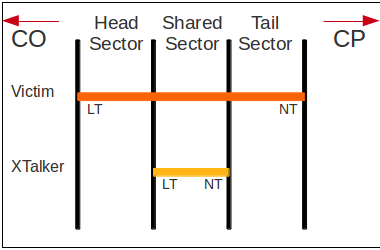
\includegraphics[width=0.35\textwidth,keepaspectratio=true]{images/FEXT_case_3.png}}
 \subfloat[Case 7]{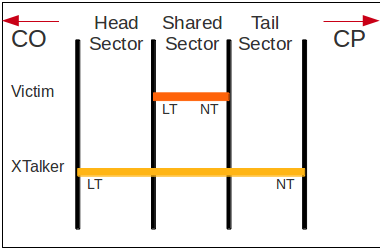
\includegraphics[width=0.35\textwidth,keepaspectratio=true]{images/FEXT_case_7.png}}\\
 \subfloat[Case 4]{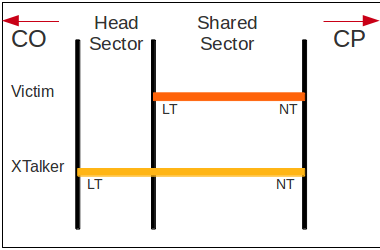
\includegraphics[width=0.35\textwidth,keepaspectratio=true]{images/FEXT_case_4.png}}
 \subfloat[Case 8]{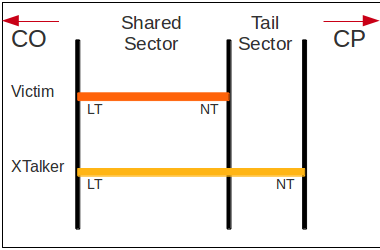
\includegraphics[width=0.35\textwidth,keepaspectratio=true]{images/FEXT_case_8.png}}\\
 \subfloat[Case 5]{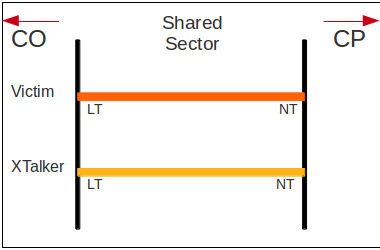
\includegraphics[width=0.35\textwidth,keepaspectratio=true]{images/FEXT_case_5.png}}
 \subfloat[Case 10]{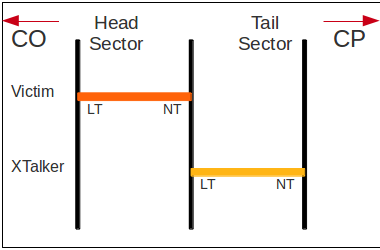
\includegraphics[width=0.35\textwidth,keepaspectratio=true]{images/FEXT_case_10.png}}\\
 % beacons-dist-lin.eps: 0x0 pixel, 300dpi, 0.00x0.00 cm, bb=
 \caption{Case-based explanation of improved FEXT modelling algorithm. Note, Case numbering rearranged to highlight upstream/downstream FEXT case inversion}
\label{fig:FEXT-xtalk-gain}
\end{figure}

As noted previously, incorporation of a Beta probability distribution sample data offsetting can be used to more accurately model the stochastic relationship in inter-line gains based on the locations of those lines in the bundle. This is accomplished by scalar multiplication of the per-channel cross-talk gain matrix with a \(N\times N\) sub-matrix of static gains measured from a 'real' bundle (See Equation ~\ref{eq:ATTFEXT}). One advantageous side effect of this appears in bit-loading of bundles with some 'identical' lines; due to the numerical instability of some bit-loading algorithms and specifically the generation of line power spectral densities, assigned bit-loads can  fluctuate violently between identical lines, producing very impulsive spectra. The relatively tiny gain adjustments applied to different identical lines in the simulated bundle present enough of a 'difference' to overcome this behaviour.

Following from the general Object Oriented architecture, and the bundle object effectively being the fundamental core of the simulation system, this object also maintains control of GPU-based algorithm specific functions, and in the case of multiple GPU operation, maintains persistent thread-pool and task queuing references within a GPU object.

The Initial stage of verification for the system was the comparison of generated Channel Matrices to those found in \cite{AM09}. Due to the different math libraries utilised between McKinley's implementation and this, direct comparison on numerical results is not reliable as a verification method, but test results obtained match those from McKinley to within IEEE floating point specifications. A better comparison is a visual one (Figure ~\ref{fig:cmComparison}).

\begin{figure}[h!]
  \centering
  \subfloat[McKinley]{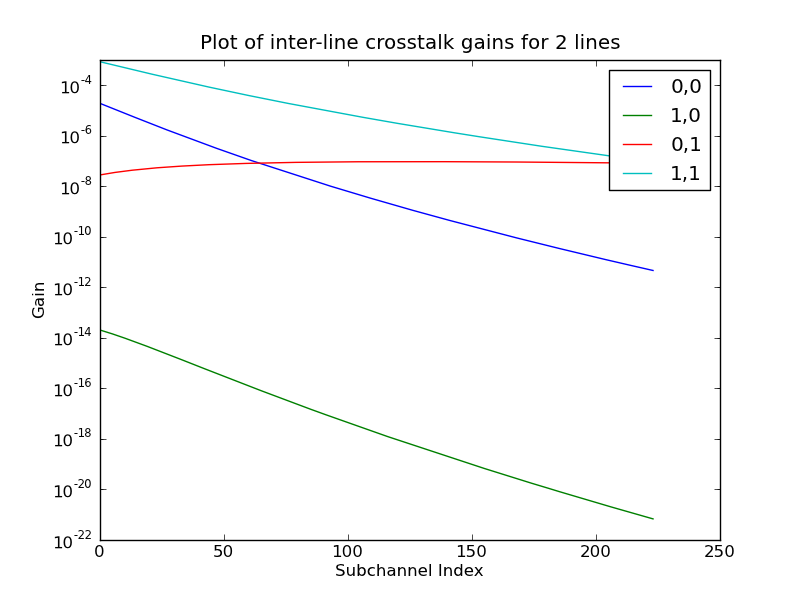
\includegraphics[width=0.45\textwidth, keepaspectratio=true]{images/2_line_channel_matrix_AMK.png}}
  \subfloat[Implementation Results]{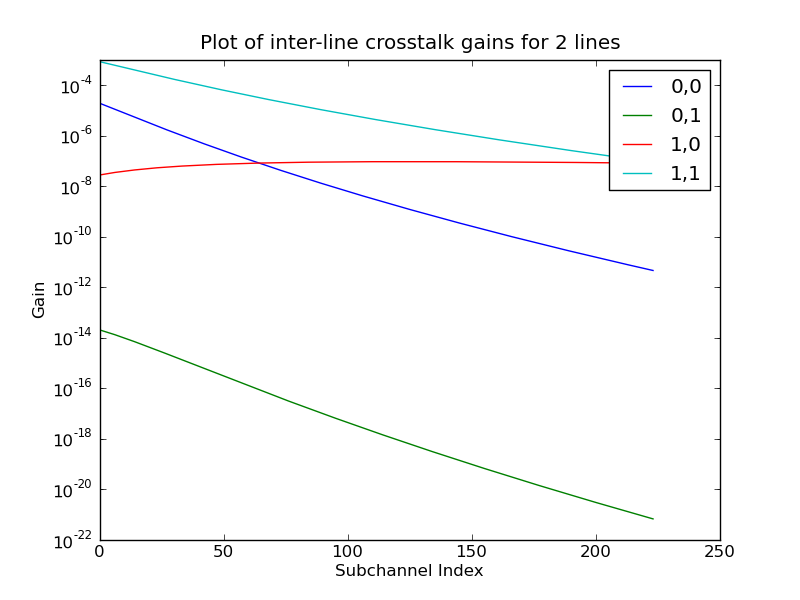
\includegraphics[width=0.45\textwidth,keepaspectratio=true]{images/2_line_channel_matrix_MINE.png}}
  \caption{Visual comparison of known-good channel matrix (McKinley) and Python implementation show that they are identical}
  \label{fig:cmComparison}
\end{figure}


\section{CPU-bound Algorithm Development and Verification}
\label{sec:algo-dev-cpu}
Before tackling the GPU implementation head on, in order to gain a more in-depth and practical understanding of the different DSM algorithms, pure Python, CPU-bound implementations of OSB, ISB and Greedy bit-loading were created. Due to the previously mentioned Object Oriented model, this process was greatly simplified by having each different algorithm class being a 'child' of a generic 'Algorithm' class; inheriting from that parent operations common to all algorithms, such as defining and instantiating universal variables, performing timing operations, verifying PSD 'sanity', file I/O functionality, and general 'build-up/tear-down' operations. This reduced the complexity of each algorithm class (slightly) and ensured that each algorithm was being tested in a consistent and repeatable fashion.

Since OSB is the 'simplest' DSM algorithm, it was implemented first (without per line rate targeting\footnote{Rate Targeting is not a focus of this project, but was explored for fun anyway}, but with PSD caching), largely from the work covered in \cite{AM09}, with operation as stated previously. Due to Python's efficient syntax and the functionality available in the Numpy math library, this was a fairly straightforward task in terms of implementing mathematical formulae in a structured way, but with commonly neglected areas such as algorithmic convergence and numerous boundary cases that are not covered in any of the technical papers cited, this was a process of iterative 'run it; it breaks; find new edge case; implement edge case; repeat'. Such edge cases range from ensuring that while PSD's can have negative values, that a negative PSD value indicates a 'failed' bit-load\footnote{And propagating this information back to the algorithm root before wasting any more processing time on this attempt} to ensuring that assigned line Lagrangian co-factor bisection did not reduce factors to infinitesimal values given very different line sections. 

The in this case, the generation of power spectral density values for each attempted bit combination is accomplished using the Numpy linear algebra library. This development and implementation was carried out in parallel with the generation of the general simulation framework. This joint development allowed for very early-stage verification of the work currently applied, specifically verification of cross-talk matrices and subsequent bit-loads against values derived from \cite{AM09} and \cite{RC04}.

The development of the line and bundle objects, as well as the general framework structure, allowing for programmatic 'hooks' for objects (classes) for different algorithms, automatic generation of post-bit-loading graph data represents more than half of the development time applied to the project\footnote{Seeing it condensed into just over a page of text is slightly depressing!}.

Verification of the OSB algorithm was done in a similar way to the verification of the gain-matrix generation; comparison with known-good results. In this case this takes the form of analysing the resultant PSD and bit assignments for the lines graphically, as shown in Figure ~\ref{fig:osbComparison}. While these do not match each other perfectly, this can be explained by two factors;propagated floating point representation differences, and updated beta-offset implementations. The McKinley implementation was built on a 32-bit floating point representation system, while the presented implementation leverages Numpy's support for 64-bit floating point values. Additionally the selected beta-offset model application in the bundle differs from the McKinley implementation in that in the McKinley model, random beta offset values are applied to the lines sequentially where in this implementation, an offset matrix is applied globally to the bundle using Numpy functionality. Given the inherent numerical instability of the calculation of the Lagrangian sum, fractional changes in cross-talk gains can significantly affect the final resultant bit-loading assignments, while maintaining a close rate-approximation between the two implementations.

\begin{figure}[h!]
  \centering
  \subfloat[McKinley Bit-loading]{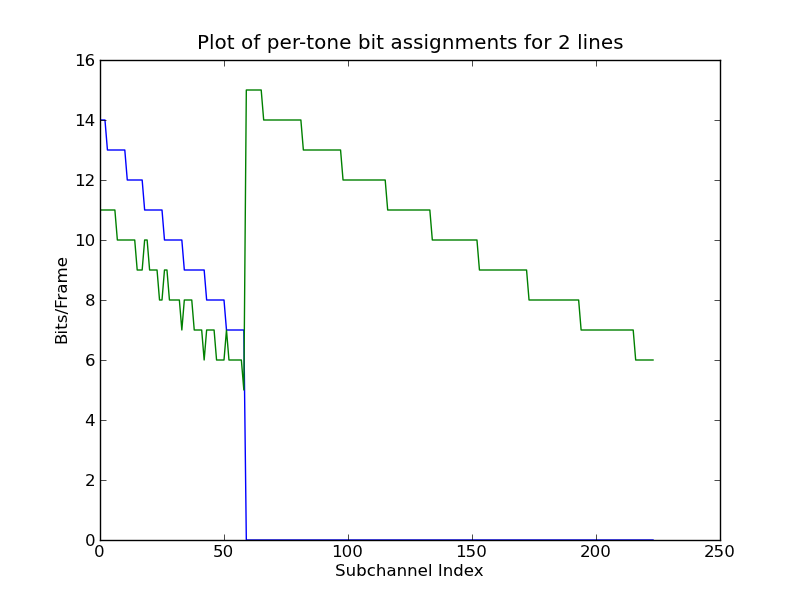
\includegraphics[width=0.45\textwidth, keepaspectratio=true]{images/2_line_bitload_AMK.png}}
  \subfloat[Implementation Bit-loading]{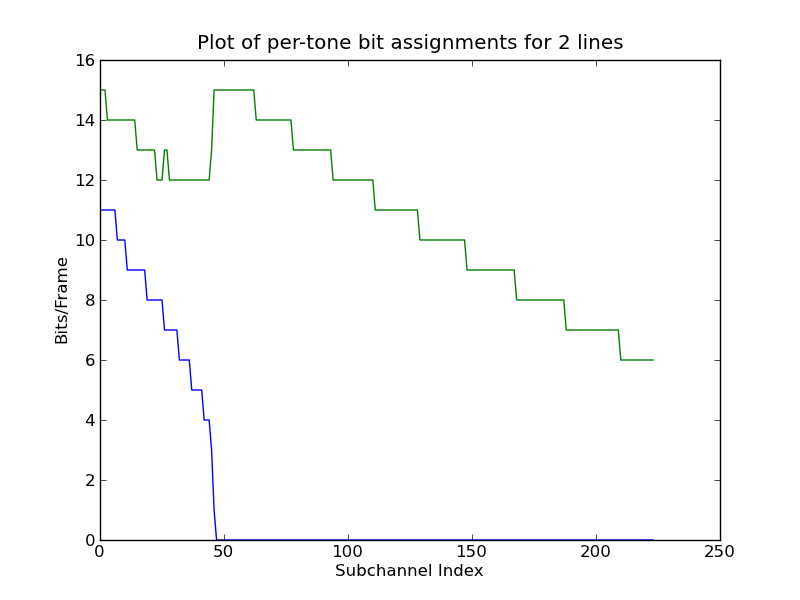
\includegraphics[width=0.45\textwidth,keepaspectratio=true]{images/2_line_bitload_MINE.png}}\\
  \subfloat[McKinley PSD]{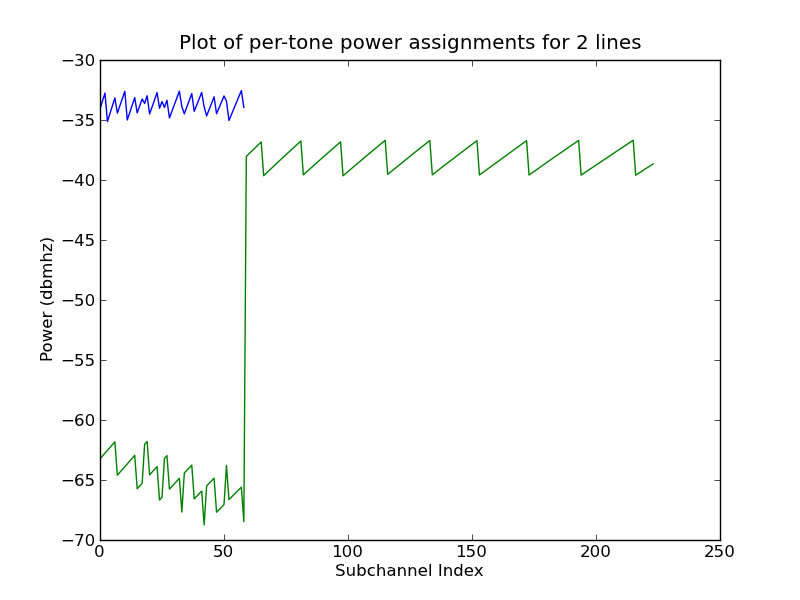
\includegraphics[width=0.45\textwidth, keepaspectratio=true]{images/2_line_power_AMK.png}}
  \subfloat[Implementation PSD]{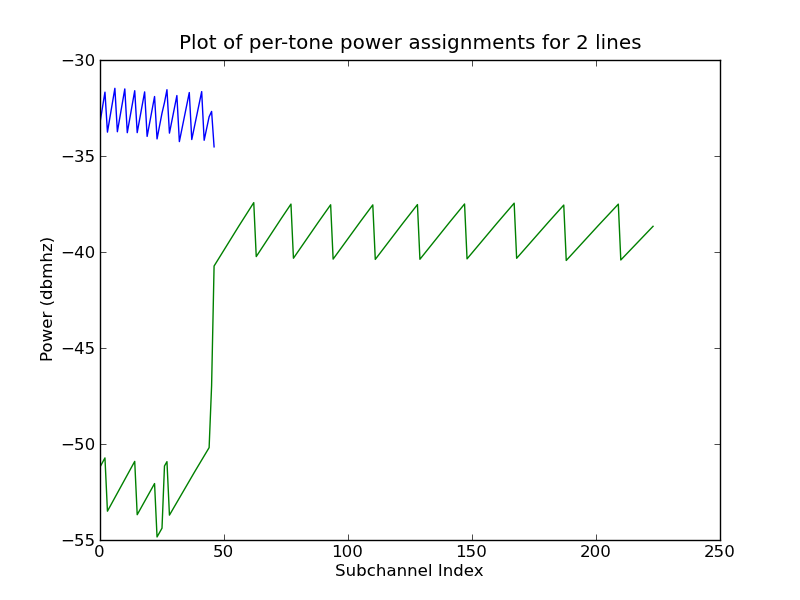
\includegraphics[width=0.45\textwidth,keepaspectratio=true]{images/2_line_power_MINE.png}}\\
  \caption{Visual comparison of known-good (McKinley) and Python implementations of OSB show that they are near-identical}
  \label{fig:osbComparison}
\end{figure}

After OSB was implemented, verified and their operation confirmed by Dr McKinley, Greedy bit-loading (MIPB) with rate targets was developed from \cite{AM09}. One modification that was made to MIPB as in \cite{AM09} was the introduction of a modified line weight updating algorithm that used the ratio-to-target rather than distance-to-target as a weight-shifting factor, giving on average half the number of iterations while maintaining expected bit-loads.\footnote{It is for this reason that MIPB results tend to be slightly skewed with respect to the McKinley implementation.}

\begin{comment}
In \cite{AM09}, three weight update schemes were presented, see Figures ~\ref{fig:mipb-rate-1}, ~\ref{fig:mipb-rate-2}, but during developement of this application, it was found that these update schemes do not converge as quickly as they could, and an alternative rate update scheme, shown in Figure ~\ref{fig:mipb-rate-mine} was implemented that, in a standard four line, three kilometer/five kilometer near-far arrangement, as in ~\ref{fig:4-3k5k-nearfar} with weights selected to be close to optimal, this alternative update converges in FIXME \% fewer iterations than the previously stated versions. As this is not a focus of this project and was simply an investigative whimsy, this will not be investigated further, other than to say that returned results are close enough to previous versions to be considered equivalent.

  \begin{figure}[h!]\label{fig:mipb-rate-1}
    \begin{algorithmic}
      \STATE FIXME
    \end{algorithmic}
  \end{figure}
  \begin{figure}[h!]\label{fig:mipb-rate-2}
    \begin{algorithmic}
      \STATE FIXME
    \end{algorithmic}
  \end{figure}
  \begin{figure}[h!]\label{fig:mipb-rate-mine}
    \begin{algorithmic}
      \FOR {\(n=1\dots N\)}
        \IF{Line Target Set}
          \STATE{\(\Delta b_n=b_n-\text{target}_n\)}
          \STATE{\(\alpha_n=\frac{\delta b_n}{\text{target}_n}\)}
          \IF{\(\text{abs}(\Delta b_n) > b_{\text{tol}}\)}
            \IF{\(\alpha_n ==  1\)}
              \STATE{\(w^+_n=1\)}
            \ELSIF{\(\alpha_n > 0\)}
              \STATE{\(w^+_n=w_n*\alpha_n\)}
            \ELSE
              \STATE{\(w^+_n=w_n*(1-\alpha_n)\)}
            \ENDIF
          \ELSE
            \STATE{\(w^+_n=w_n\)}
          \ENDIF
        \ELSE
          \STATE{\(w^+_n=w_n\)}
        \ENDIF
      \ENDFOR
    \end{algorithmic}
  \end{figure}
\end{comment}

An implementation of ISB soon followed, and verified in the same manner. One particular additional version was made of the ISB algorithm in preparation for GPU parallelisation; loop reversal of the inner optimisation step. 'Classic' ISB iterates over each line individually, internally repeating bit incrementing steps until bit-load convergence is achieved, shown in Figure \ref{fig:isb-standard-loop}. An alternative but equivalent loop construct is to do the per-channel incrementing inside a global bit-convergence loop, as shown in Figure \ref{fig:isb-alternate-loop}. This manipulation is safe since each channel is ideally independent to the power conditions of other tones.

\begin{figure}[ht!]
  \begin{algorithmic}
    \FORALL{channels}
      \REPEAT
        \FORALL{lines}
        \STATE{\(\text{argmax}_{b_k}L(k)\)}
        \STATE{By 1-d exhaustive search}
        \ENDFOR
      \UNTIL{Bit-load Convergence}
    \ENDFOR
  \end{algorithmic}
  \caption{Standard ISB Loop construct}
  \label{fig:isb-standard-loop}
\end{figure}

\begin{figure}[ht!]
  \begin{algorithmic}
    \REPEAT
      \FORALL{channels}
        \FORALL{lines}
        \STATE{\(\text{argmax}_{b_k}L(k)\)}
        \STATE{By 1-d exhaustive search}
        \ENDFOR
      \ENDFOR
    \UNTIL{Bit-load Convergence}
  \end{algorithmic}
  \caption{Exchanged ISB Loop construct}
  \label{fig:isb-alternate-loop}  
\end{figure}

As part of second-stage verification and re-factoring, significant functional portions of OSB and ISB were moved into the Algorithm super-class, such as lambda bisection and rate metric functions, since both algorithms do largely the same thing within the outer loops of the implementation. Since the only differences between the two algorithms is their inner optimisation function, these are included in this document as Appendices \ref{apx:osb-optimise-p-cpu} and \ref{apx:isb-optimise-p-cpu}.

For completeness, figure \ref{fig:mipbComparison} and \ref{fig:isbComparison} show like for like comparison of bit load and power spectra between this solution and the McKinley implementation given a standard two line near-far scenario (as shown in \ref{fig:2-3k5k-nearfar})\footnote{Notice that occasionally the low-channel bit-allocations are swapped between the two lines, i.e. line A in McKinley may have the bit-allocation of line B in this implementation below channel 50. Consultations with McKinley state that this behaviour is acceptable.}

\begin{figure}[h!]
  \centering
  \subfloat[McKinley Bit-loading]{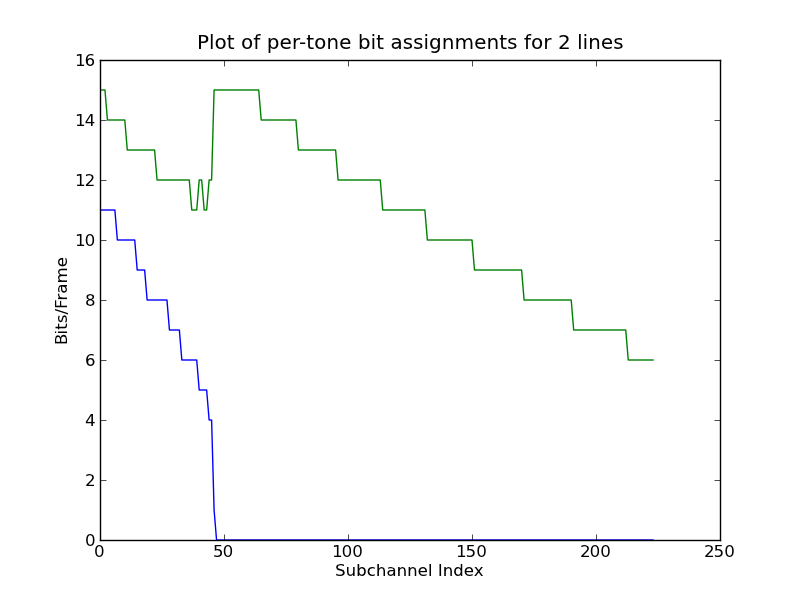
\includegraphics[width=0.45\textwidth, keepaspectratio=true]{images/b_and_p_stats_2lines_near_far_mipb3g_224_371_2451-bitrate.png}}
  \subfloat[Implementation Bit-loading]{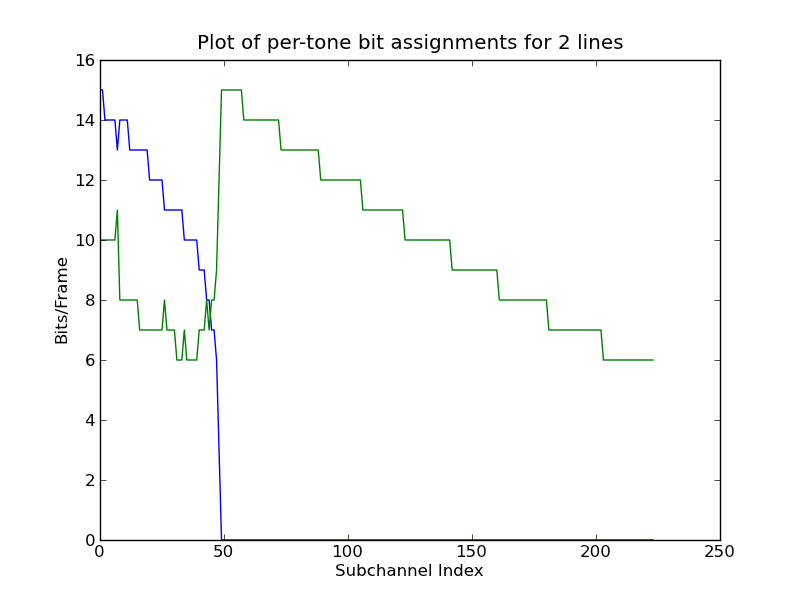
\includegraphics[width=0.45\textwidth,keepaspectratio=true]{images/mipbtest2-bitrate.png}}\\
  \subfloat[McKinley PSD]{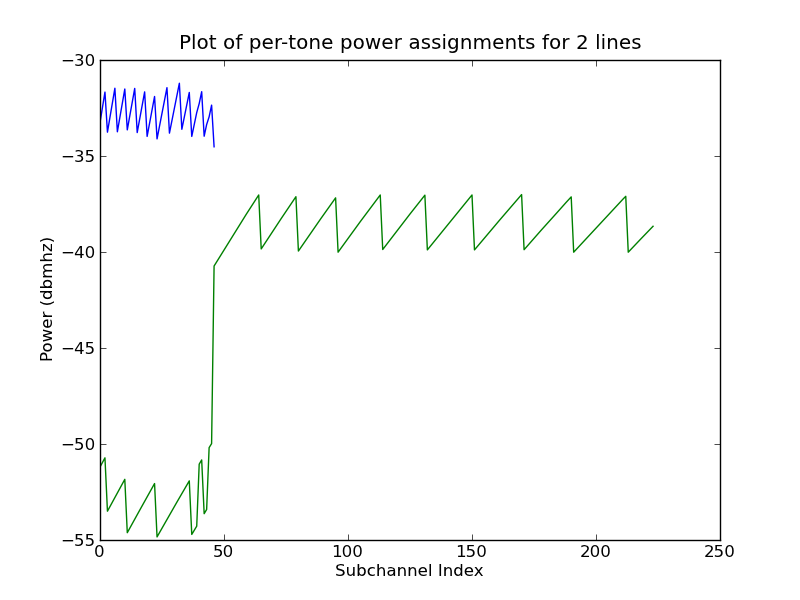
\includegraphics[width=0.45\textwidth, keepaspectratio=true]{images/b_and_p_stats_2lines_near_far_mipb3g_224_371_2451-power.png}}
  \subfloat[Implementation PSD]{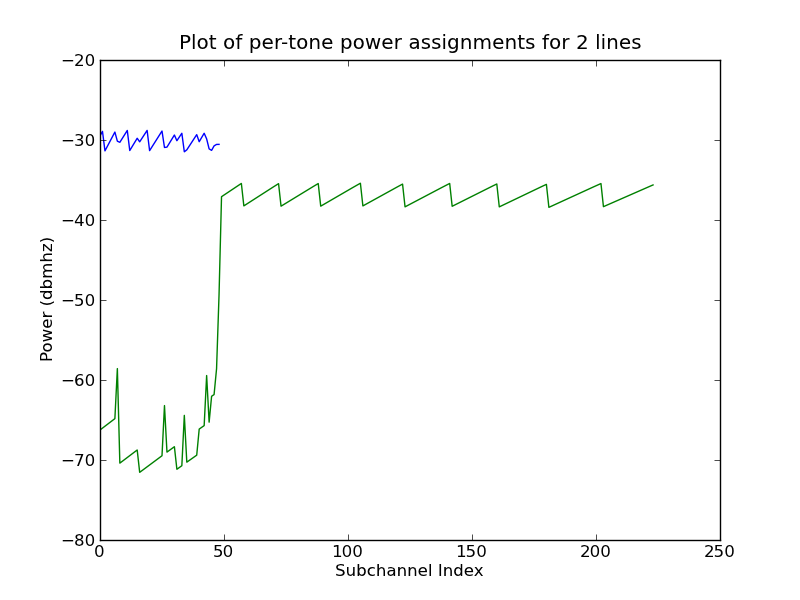
\includegraphics[width=0.45\textwidth,keepaspectratio=true]{images/mipbtest2-power.png}}\\
  \caption{Visual comparison of known-good bit-load and power spectra for Greedy (MIPB), with rates targeted to OSB, show that the implementations are equivalent}
  \label{fig:mipbComparison}
\end{figure}

\begin{figure}[h!]
  \centering
  \subfloat[McKinley Bit-loading]{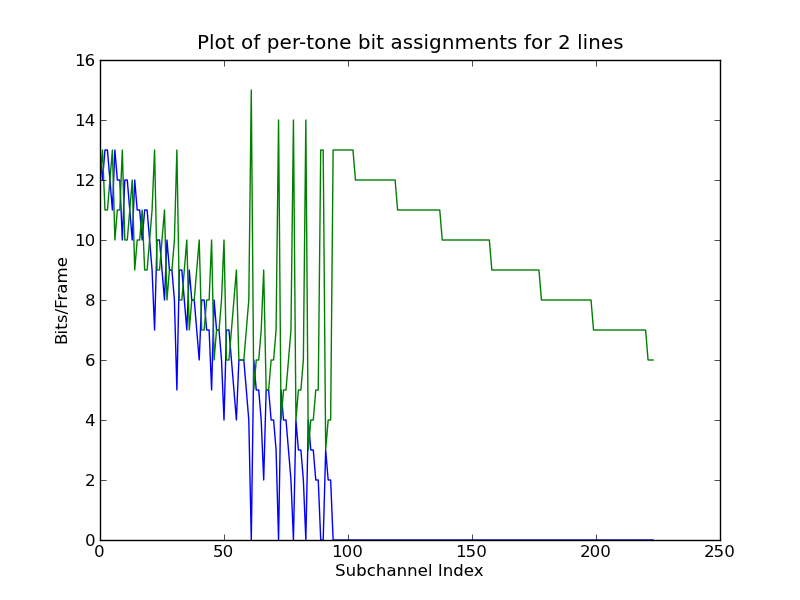
\includegraphics[width=0.45\textwidth, keepaspectratio=true]{images/b_and_p_stats_2lines_near_far_ISB_224-bitrate.png}}
  \subfloat[Implementation Bit-loading]{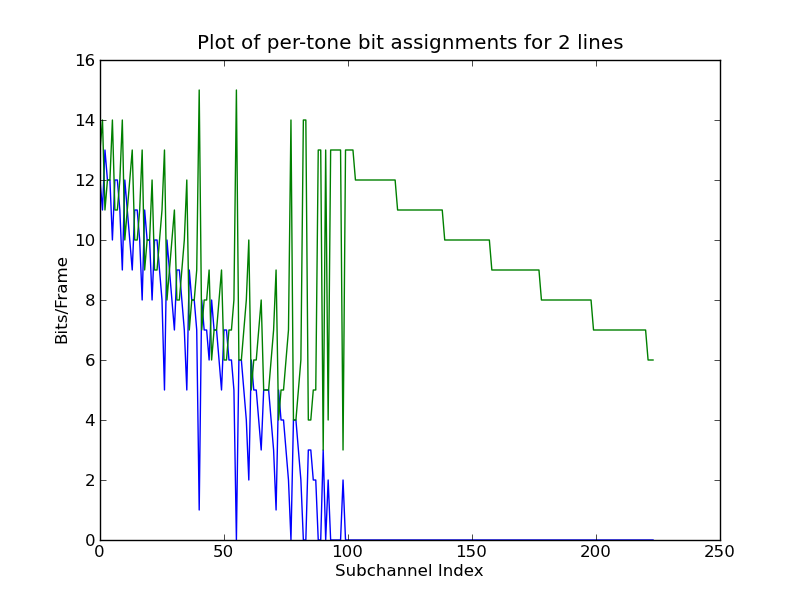
\includegraphics[width=0.45\textwidth,keepaspectratio=true]{images/ISB_2-3k_5k-near_far_CPU-bitrate.png}}\\
  \subfloat[McKinley PSD]{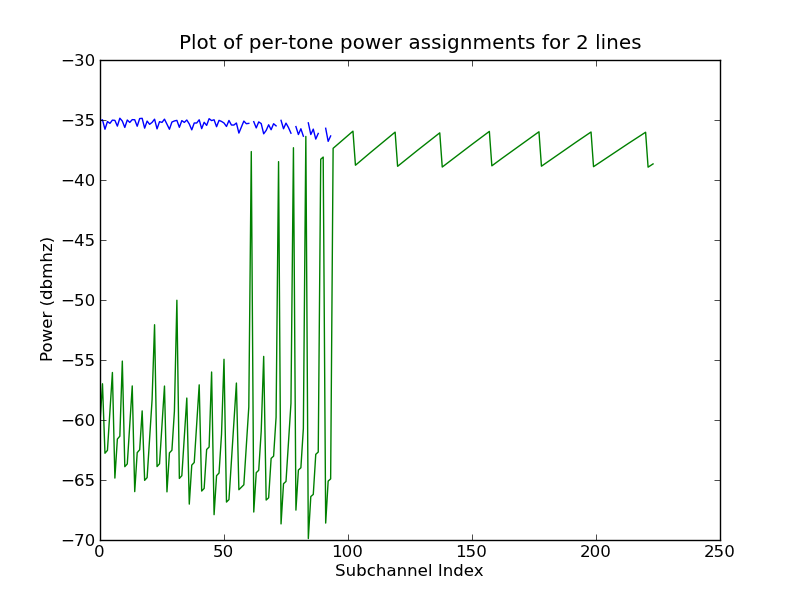
\includegraphics[width=0.45\textwidth, keepaspectratio=true]{images/b_and_p_stats_2lines_near_far_ISB_224-power.png}}
  \subfloat[Implementation PSD]{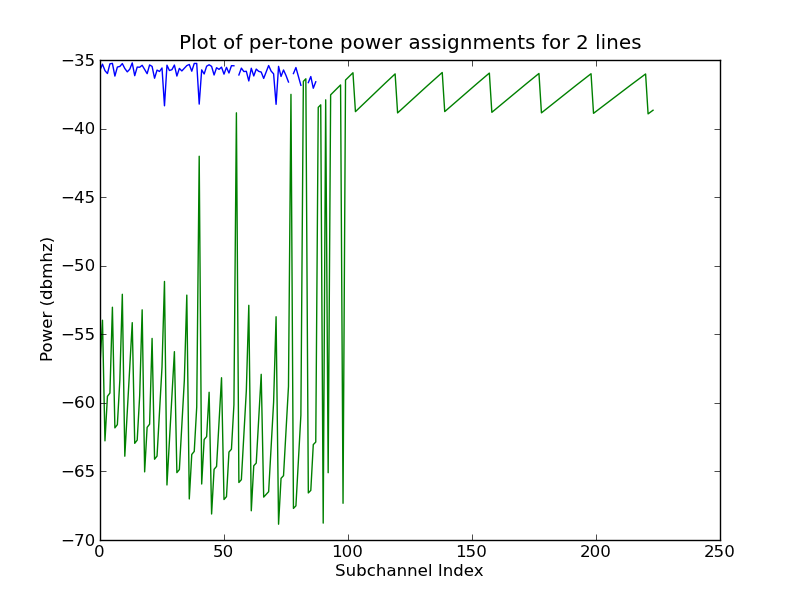
\includegraphics[width=0.45\textwidth,keepaspectratio=true]{images/ISB_2-3k_5k-near_far_CPU-power.png}}\\
  \caption{Visual comparison of known-good bit-load and power spectra for ISB, show that the implementations are equivalent}
  \label{fig:isbComparison}
\end{figure}

\section{GPU-bound Algorithm Development}
\label{sec:algo-dev-gpu}
\subsection{Retrospective analysis of CPU bound applications}
Python's profiling architecture allows for detailed analysis of 'hot-zones' within applications, i.e. the areas within a program where most time and resources are spent over the course of execution. In order to see a 'practical' workload, for the following analysis, a four line near-far bundle was used\ref{fig:4-3k5k-nearfar}.
In order to visualise the profiled-executions, the RunSnakeRun application was used to generate squaremap representations of time spent in different functions; larger areas represent a greater total time spent in that area of computation (Figure \ref{fig:cpuprofileComparison}). 
\begin{figure}[h!]
  \centering
  \subfloat[OSB Profile SquareMap]{\label{fig:cpuprofileOSB}\includegraphics[width=0.75\textwidth,keepaspectratio=true]{images/OSB_4_profile_CPU.png}}\\
  \subfloat[ISB Profile SquareMap]{\label{fig:cpuprofileISB}\includegraphics[width=0.75\textwidth, keepaspectratio=true]{images/ISB_4_profile_CPU.png}}\\
  \subfloat[MIPB Profile SquareMap]{\label{fig:cpuprofileMIPB}\includegraphics[width=0.75\textwidth,keepaspectratio=true]{images/MIPB_4_profile_CPU.png}}\\
  \caption{SquareMap output from RunSnake showing percentage execution time for a four line bundle scenario}
  \label{fig:cpuprofileComparison}
\end{figure}

\subsubsection{Conclusions}
From these profiling investigations, it is clear that the largest computational bottleneck is the calculation of power spectral densities for different bit-load combinations. This is exemplified particularly in OSB and ISB; the Lagrangian calculations ('L\_k') clearly take up the vast majority of computation time, and in the case of MIPB, the culprit is the recalculation of the \(\Delta p\) values per tone; again, the primary operation is calculation of PSD's. As previously discussed, OSB and ISB, from an algorithmic perspective, lend themselves to parallelisation, but the lack of on-board linear algebra library to calculate individual \(N\times N\)-system solutions is a serious problem; under-test, using the cuBLAS library to calculate \(4\)-system solutions was actually 4\% slower than using the built-in Numpy linear-algebra system on the CPU side\footnote{To try and make this test fair, The calculation was repeated 256 times with pre-generated random inputs on both the GPU and CPU side, with these repeats parallelised on the GPU}. It is clear that for such small matrices, there is no advantage to using standard GPU libraries. And unfortunately, no alternative libraries could be found, and since the CUDA device cannot access any host data, C implementations such as GSL, LAPACK, LINPACK, or EIGEN could not be used.
This leads to the need to create a custom, stripped down, linear system solver\footnote{This was quite possibly the most technically difficult and frustrating section of the entire project}.

Source code is availiable from https://bitbucket.org/bolster/multiuserdsm for all of the applications (and more) used within this project.

Due to the numerical instability of the systems involved, the linear solver must be able to handle arbitrary matrices, as well as being able to gracefully handle failure without bringing the whole GPU down. This led to the selection of a customised maximally pivoted LU Decomposition algorithm\footnote{A Blog post discussing the development of this function is availiable at http://bit.ly/eH3WH6}, pieced together from \cite{WHP92},\cite{GR10}, \cite{JDJZW03} and \cite{GOU96}, and the final solution arrived at is shown in Appendix \ref{apx:cuda-linalg-solver}. This algorithm does not leverage CUDA parallelism. The reason for this is two fold; a natural parallelisation scheme for this algorithm would be for a collection of threads to collaboratively work on a single matrix, but this arrangement would not efficiently occupy the GPU's processing units until the number of lines being tested was greater than at least 8. A Secondary reason is that from the perspective of OSB, having each block calculate a single bit-permutation would greatly limit the number of permutations able to be tested simultaneously, and as such the same kernel that could optimally handle up to \(2^{16}\) permutations (for example, four lines) in one execution would have to be executed eight times to compute the same result. Further, due to the conditional nature of LU Decomposition, utilising per-thread solving on locally related datasets reduces the total amount of warp divergence, increasing overall speed. Experimentally, using block-shared matrix solving was approximately 23\% faster than thread-solving for single executions, but when put into a realistic cradle of input values and ranges, was 15\% slower. This was largely due to the need for repeated executions, as well as the previously stated warp-divergence issues.

The profile results also show that the calculation of optimise\_p is the section of the OSB and ISB algorithms most heavily in need of optimisation. To note in this section is the difference in how the ``asarray.numeric'' numpy functions within optimise\_p are executed between OSB and ISB; these functions are involved in the PSD caching operation; every time a PSD value is requested, the function arguments are hashed, and a dictionary of past values is searched for that hash. This operation greatly reduces the number of linear algebra operations performed in OSB especially (attaining a cache hit ratio of over 98\%, meaning that the algorithm only needs to execute 2\% of the time that it is actually called)\footnote{ISB has a lower, but still significant, cache hit ratio of just over 80\%, but since ISB executes approximately 5\% the number of PSD calculations as OSB, this caching is less significant. MIPB by comparison has a hit ratio of 0\%; no PSD is asked for twice, so caching is largely useless unless using rate targeting, and even then hit ratios average between 10-20\%.}, but does so at the expense of system memory (for a six line network, this cache easily exceeds 8GB). If the calculation of the PSD's can be sufficiently accelerated, this cache could be done away with completely, greatly reducing the total memory footprint of the system, and therefore the cost of execution.

\subsection{OSB: Avenues of parallelisation and problem decomposition schemes}
OSB power optimisation is a naturally parallel algorithm; calculating all possible permutations for all users for all channels, finding the Lagrangian for the best combination on each channel, and loading it. This multiple-level parallelism makes it perfect for GPU execution, but also for multiple GPU execution; each GPU can be assigned blocks of channels or using a channel queue, while each device computes all the permutations for that channel.
Power Optimisation in OSB has three distinct sections; Generation of A and B matrices from individual bit-load permutations, PSD calculation for each permutation, and Lagrangian calculation for that PSD using assigned lambda and weight values. This leads to the possibility of using three independent kernels, with persistent memories across executions (i.e. no need to move memory around during a single optimisation).

This logical decomposition presents another opportunity to leverage the power of CUDA. Using different block and grid dimensions, each kernel's execution could be customised to use a variety of thread and block level parallelism; for instance \(N\) threads could work in parallel within each block to generate the A and B matrices for solving the PSD of each permutation\footnote{As Derived from equation \eqref{eq:DSLSystemModelAlt}}, then individual threads would solve that system, and subsequently calculate the Lagrangian for that permutation, returning a vector of Lagrangian values such that the host process can take the maximum index from that vector and deterministically regenerate the bit-load that created it, as well as retrieving that permutations PSD from the device, completely removing the CPU from PSD generation.

\subsection{Greedy: Avenues of parallelisation and problem decomposition schemes}
Due to the incremental step-wise operation of Greedy bit-loading, and after thorough consultation with Dr McKinley, there is no efficient way to parallelise Greedy without fundamentally changing the operation of the algorithm. To demonstrate this, a 'best-attempt' parallelisation was made, focusing on the updating of tonal costs. After the first step in the algorithm, this is exclusively done on a per-tone basis, meaning that at most, \(N\) values are being generated at once. This produced a slow-down of 23\% when compared to the CPU-bound algorithm against a 6-line bundle, predominantly due to memory transfers between the host and the device.

As such, Greedy must be disregarded from this project, but will be used as a comparison to answer the question 'Can Massive Parallelism compete with algorithmic improvement?'\footnote{Without going any further, I would be confident that this is false for greater than 6 lines; Greedy is just that fast}.

\subsubsection{ISB: Avenues of parallelisation and problem decomposition schemes}
ISB, even though its very close in structure to OSB, presents an interesting predicament; while it is still the power optimisation that is the major workload, the incremental operation of this section of the algorithm makes it initially quite difficult to see how to efficiently parallelise it. At first blush, the same patter as OSB could be followed; where independent channels are separately computed independently, allowing for simple multi-device distribution, or as mentioned, to iterate over the incremental bit combinations of the entire bundle, excluding 'simple' multiple device execution.

In the former case, the style of Figure \ref{fig:isb-standard-loop} would be adopted, where each kernel invocation could iteratively perform optimisation on each particular channel. The difficulty is that this algorithm could not really be parallelised any further due to the incremental nature of ISB. It is possible that this could be split up by each user attempting their own bit-load permutation individually, with a record of 'best' bit-load shared between threads in a block, but this is a fundamental break in the ISB algorithm, so would not be guaranteed to be either near-optimal, or even converge at all.

The second option appears to be the most viable, if (at first glance) less applicable to multiple devices. Using an iteration construct like Figure \ref{fig:isb-alternate-loop}, each thread-block could perform each channel's line-loop optimisation. This would only involve a constantly defined loop within the CUDA kernel, which is significantly more performant than a non-deterministic convergence condition as would be required in the former case. In short, this structure would perform channel and permutation parallelism, with each block containing 16\footnote{The number of possible bit-load combinations for the line currently being looped over within the kernel} threads. While this is not a huge number of threads, it's enough to sufficiently occupy the device. Additionally, CUDA's shared memory space can be used such that at each loop, a block-shared store of the running-bit-load would be updated on each per-line optimisation, containing the bit-permutation with the highest Lagrangian. With 224 ADSL channels, there is no reasonable condition under which this would require more than one device (\(\text{Number of Threads}=B_{\text{max}}\times K\)), but if desired, the channel range could be partitioned across devices.

While the first option will be explored, but the second will be the focus of most development time.

\subsubsection{Development of generalised GPU workload sharing model}
One of the most significant drawbacks of CUDA is its computational simplicity; that is to say that CUDA has relatively little workload partitioning and runtime optimisation when compared to systems such as OpenCL or OpenMP. As such, and from the insights found previously in this section, a generalised workload model was developed to produce near-optimal grid and block dimensions for generic kernels. Although these design patterns are configured with the computation of single PSD/Lagrangian calculations in mind, the same theories of block, warp, grid and device partitioning can easily be applied to any computing problem on GPU's\footnote{as long as those problems are independent of each-other}.

Each CUDA device has an optimal occupancy ratio for a particular kernel, involving the number of SP's available on the device, expected memory accesses, etc., and as such these patterns will not be perfect. They are simply 'quite good', and attempt to dynamically assess optimal block and grid assignments based on individual hardware configurations without having to inspect the kernels being executed. The first of these patterns is a per-device workload calculation. This queries the device for information such as the number of SP's, number of threads per warp, and the maximum permitted threads per block \footnote{Note, this is not the optimal number of threads, just a ceiling value}.

Given a maximum value of 'workload', in this case the number of thread executions ideally desired, the number of warps that this workload requires is calculated. This is scaled to the number of threads per warp and rounded up to the nearest multiple of the warp size (usually 32) to give an optimal 'thread per block' count. This value is then used, along with a maximum thread-count ceiling, termed 'gridmax', to find the optimal number of blocks to execute these threads within while staying within device limits. The python code for this function is shown in figure ~\ref{fig:workload-calc}. Note that this code is developed for 1-D grids and blocks, but could easily be extended for multi-dimensionality or for cooperative thread execution.

\begin{figure}[H]
  \lstinputlisting[language=Python]{sourcefiles/workload-calc.py}
  \caption{Sanitised Python function for near-optimal Grid and Block dimensions for thread-independent operations}
  \label{fig:workload-calc}
\end{figure}

\subsubsection{Development of generalised multi-device function queue}
A GPU device and a host process must be paired, i.e., one host-bound process can execute CUDA kernels on only one GPU device \footnote{This has changed in CUDA 4.0 RC2, but due to PyCUDA's current lack of direct hooks into this functionality, this option could not be explored sufficiently for inclusion in this document}. This restriction, coupled with Python's Global Interpreter Lock (GIL), which is a mutex that prevents multiple native threads from executing Python byte-codes simultaneously\footnote{This is required due to Python's memory management system not being thread-safe}, requires that for multiple GPU devices to me leveraged, additional multi-processing structures must be used.

There are two major families of multiprocessing structures in Python; one that leverages system threads, like Unix pThreads, in a module called 'threading', and a second that uses full processes, akin to OpenMP. The threading model was selected as the use of multiple processes requires that the entire application (or at least the sections of the application that must deal with multiprocessing) be immutable. This disallows the use of class instance methods (such as all of the bundle and algorithm class functions). Further, processes are significantly 'larger' in terms of memory allocation, and significantly slower in terms of process forking, when compared to the lightweight threading model.

As such, the generated GPU class, was augmented with a secondary class of persistent GPU threads. These objects, once instantiated with a GPU device index on application start-up, wait on work items to be put one a queue by the GPU parent class. Once a work item is received, the appropriate internal method for each algorithm is selected and executed on the GPU to which it has been instantiated. The advantage of this queueing method is that work is inherently balanced across devices without any declared load-balancing algorithm since as soon as each thread has completed its current work item and returned its results to the parent class, it simply picks the next free item from the queue.

The overheads incurred in this process are insignificant, and generally hidden; since CUDA executions are none blocking (i.e. unless told explicitly to wait, a host process can continue to process other information during kernel running time), and that these threads are persistent. This persistence is important, since in the single GPU model, each method execution the GPU device must be reinitialised every time the method is called. With this threading model, each device is initialised once during application start-up, and this initialisation time can be hidden behind other work being done such as the generation of the bundle channel matrix.

Further, this threading model allows the application to be device and system agnostic; automatically adapting to a single, twin, or quad-device system with no user action. This combined with the previously mentioned near-optimal workload calculation could even allow for mixed device systems\footnote{Although this functionality has not been tested, since no systems were available for test operated under a mixed-device configuration}.

\section{GPU Solutions and Verification}
The solutions arrived at for GPU consist of a series of C-sourced CUDA kernels, along with a collection of device-side functions. While PyCUDA exposes some high-level GPU abstraction capabilities, such as parallel per-element array manipulations, this avenue of work could not be applied cleanly to the problem set, mainly due to the need for intra-element operations such as PSD solving.

Before diving into details; the OSB solution consists of three separate per-channel kernels that replicate the operation of 'optimise\_p' in the serial implementation (Bit-load/AB generation, PSD Solving, LK calculation), executing for all bit-load permutations simultaneously; while ISB consists of a single kernel that performs per iterative optimisation across a range of channels simultaneously, with the kernel being iteratively executed until bit-load convergence\footnote{Strictly speaking, these calculations are not simultaneous, as individual warps are swapped in and out of the SM's, but for the sake of simplicity, 'simultaneously' is used}.

Additionally, a secondary function was generated for global verification of 'optimal' bit-load PSD's, used during final recalculation of per-line power ratings.

These kernels and device functions are shown in detail in Appendix \ref{apx:GPU-code}

\subsection{OSB GPU}
In the OSB solution, the full permutation range is sliced based on the maximum efficient capacity of the device being used; this generally allows for a maximum three-line solution to be found in 'one shot', but since OSB permutations are computationally explosive, often the kernel triplet is executed many times to span this permutation range to arrive at an optimal solution for a single channel.

This kernel triplet consists of:
\begin{itemize*}
\item{'lk\_osb\_prepare\_permutations': Generate A and B matrices for PSD calculation of all bit permutations}
\item{'osb\_solve': Solve all permutation's PSD's in parallel}
\item{'lk\_max\_permutations': Solve all permutation's PSD's in parallel}
\end{itemize*}
The reason for the separation is partly logically and partly technical; the generation of A and B matrices is made parallel in both the permutation and line ranges, as each A/B generation shares many values for each respective permutation. Therefore the block and grid dimensions for CUDA execution were set so as to enhance memory coalescing and column-major shared memory accesses; each 'block' calculates one permutation, and each thread within the block calculates one row of A and B. The Solving and LK generation kernels do not easily exhibit this level of parallelism and as such are executed under a thread-share model; i.e. each thread is independent but grouped as a 'best attempt' at efficient memory access.

As this algorithm operates on a per-channel basis, the major input data (the cross-talk gain matrix) can stay resident on the device for the complete execution of one channel, reducing the time spent transferring data to and from the device. Additionally, this algorithm allows access to not only the optimised bit-load, but also to the PSD of that bit-load, which remains resident in device memory. This reduces repeat-calculations.

After each kernel execution, as CUDA has no rational way to perform linked-reductions (such as \(\text{argmax}\)), the device array containing LK values is returned to the host, and the maximal LK-permutation found from the array-index. If this LK value exceeds the current global maximal LK, then the PSD for that value is also pulled from the device, and returned to the calling function.

The multi-device extension to this implementation is a simple queue-based channel distribution across devices, as discussed previously. An attempt was made to distribute permutation slices instead of channels, but due to excessive memory redundancies (i.e the same cross-talk gain matrix having to be constantly sent to the host) this implementation was significantly slower that the channel-distributed model\footnote{For four line OSB, the permutation sharing implementation encountered a versus-CPU speed-up of 3x, compared to, as we'll see later, a channel-distributed speed-up of 10 on a single GPU}.

\subsubsection{Verification}
The natural verification method is to compare returned PSD's against the previously-verified CPU implementation (Figure \ref{fig:cpugpuOSBComparison}). What is interesting about this result is that while power allocations match almost perfectly, bit allocations differ, it appears, significantly. This is due to the inherent numerical instability of the Lagrangian maximisation method. In relative terms, single-differences in bit allocations correspond to minimal PSD changes, and the absolute difference in total bit-load between CPU and GPU versions is less than 35 bits-per-frame over the entire bundle.

As this is an investigation into the viability of GPU implementations and not a study in their correctness, it is felt that this is an acceptable margin of error.

This verification stands for both single and multi-GPU executions.
\begin{figure}[H]
  \centering
  \subfloat[OSB CPU Power Allocation]{\includegraphics[width=0.45\textwidth,keepaspectratio=true]{images/OSB_3-3k_5k-near_far_CPU-power.png}}
  \subfloat[OSB GPU Power Allocation]{\includegraphics[width=0.45\textwidth, keepaspectratio=true]{images/OSB_3-3k_5k-near_far_GPU-power.png}}\\
  \subfloat[OSB CPU Bit-load]{\includegraphics[width=0.45\textwidth,keepaspectratio=true]{images/OSB_3-3k_5k-near_far_CPU-bitrate.png}}
  \subfloat[OSB GPU Bit-load]{\includegraphics[width=0.45\textwidth, keepaspectratio=true]{images/OSB_3-3k_5k-near_far_GPU-bitrate.png}}\\
  \caption{Comparison of three line, near far scenario OSB: CPU/GPU}
  \label{fig:cpugpuOSBComparison}
\end{figure}
\subsection{ISB GPU}
In the ISB solution, the host thread iteratively calls a single kernel that operates on all channels simultaneously, 'isb\_optimise\_inc', that increments across each line and updates a shared 'optimal' bit-load for that iteration. The kernel is repeatedly called until the bundle/sub-bundle bit-load has converged\footnote{Sub-bundles in the case of multi-GPU operation}.

This kernel operates on a mixed-thread-share model, where each block within the CUDA grid calculates the optimal load for a single channel, and each thread within the block performs the PSD and LK calculations for the line being iterated upon. As such, the 1-D grid takes the form \([K|B_{\text{max}}]\). Each block maintains a shared memory location for the 'best' bit-load permutation from each successive line-round, and thus collects an 'optimal' bit-load across all lines on that channel. As such, strictly speaking this kernel is not limited by the number of lines, but by how long it takes for the bit-loads to converge \footnote{Experimentally it has been found that this implementation of ISB can happily operate on at least 16 line bundles within a practicable time frame(24 seconds), and the only reason for not going further than that is the constraints of 32-bit numerical representation of bit-permutations}

\subsubsection{Verification}
Again, the simplest way to verify operation is direct comparison to CPU bound implementations (Figure \ref{fig:cpugpuISBComparison}) In this case the graphs tell a very different story than that of OSB; as can be seen, the GPU implementation has power convergence problems between the green and red lines, but the bit-loads applied are nearly a perfect match. This is again due to numerical representation problems, where by the PSD/LK calculations produce vanishingly small differences between these two line segments, leading to oscillation of bit-load allocations across these lines. Again, the end result of this is a global bundle rate that is within 3\% margin of error between CPU/GPU implementations.
\begin{figure}[H]
  \centering
  \subfloat[ISB CPU Power Allocation]{\includegraphics[width=0.45\textwidth,keepaspectratio=true]{images/ISB_3-3k_5k-near_far_CPU-power.png}}
  \subfloat[ISB GPU Power Allocation]{\includegraphics[width=0.45\textwidth, keepaspectratio=true]{images/ISB_3-3k_5k-near_far_GPU_1-power.png}}\\
  \subfloat[ISB CPU Bit-load]{\includegraphics[width=0.45\textwidth,keepaspectratio=true]{images/ISB_3-3k_5k-near_far_CPU-bitrate.png}}
  \subfloat[ISB GPU Bit-load]{\includegraphics[width=0.45\textwidth, keepaspectratio=true]{images/ISB_3-3k_5k-near_far_GPU_1-bitrate.png}}\\
  \caption{Comparison of three line, near far scenario ISB: CPU/GPU}
  \label{fig:cpugpuISBComparison}
\end{figure}

\subsection{MIPB GPU}
No MIPB solution attempted was functional; as stated, MIPB as it stands has no direct parallelisation vector. Work is under way to perform parallel pre-computation of bit-load chains, but as this is a fundamental divergence from this reports aim, it is not within the scope of this discussion.

%\chapter{Tools and Software}

There are a number of tools and software elements required in the creation of this project, as outlined in section \ref{sec:arch} and the project specification (section \ref{sec:proj-spec}). To engineer the best solution, it is important to fully understand the operation of each of these elements and explore their implementations and limitations. Thus to aid the engineering process, each of the elements to be used are explained in this chapter, as well as an evaluation of the choices for the server.

  \section{Click Modular Router}
    \label{sec:click}
    Click is a software architecture for building extensible and configurable routers\cite{EKRM+00}, designed as the Ph.D. project of M.I.T. graduate Eddie Kohler. The design of the Click software structure is modular in which each individual module is called an element. Each of these elements performs simple packet processing tasks on a per packet basis. Connecting these modules in a 'flow', it is possible to develop complex and powerful tasks from a simple configuration file.

    \begin{figure}[H]
      \centering
      \lstinputlisting{../files/test-device.click}
      \caption{Example Click configuration file}
      \label{fig:click-file}
    \end{figure}
    \begin{figure}
      \centering
      \includegraphics[width=10cm,height=5cm,keepaspectratio=true]{../images/test-device.pdf}
      \caption{Visual representation of click flow in figure \ref{fig:click-file}}
      \label{fig:click-ex}
    \end{figure}

    The source code and corresponding diagram in figures \ref{fig:click-file} and \ref{fig:click-ex} show three click elements combined to perform a very simple task. The \texttt{FromDevice()} element interfaces with the hardware's \texttt{ath0} device, the \texttt{Print()} element prints an 'OK' message every time it processes a packet, and the \texttt{Discard()} element cleanly deletes the packet. These elements are C++ objects and are designed to be fine-grained with simple specifications. It is the Click ethos that many fine-grained, simple elements are preferable to few coarse-grained, complex elements. New elements can be created to perform tasks that are not fulfilled by the packaged elements with the click install. The three most important properties of each element are described below and illustrated in figure \ref{fig:click-tee}.\cite{EKRM+00}

    \begin{enumerate*}
    \item\textbf{Element Class}\hfill\\Each element belongs to one element class. This specifies the code that should be executed when the element processes a packet, as well as the element’s initialisation procedure and data layout.
    \item\textbf{Ports}\hfill\\An element can have any number of input and output ports. Every connection goes from an output port on one element to an input port on another. Different ports can have different semantics; for example, second output ports are often used to emit erroneous packets.
    \item\textbf{Configuration Strings}\hfill\\The optional configuration string contains additional arguments that are passed to the element at router initialization time. Many element classes use these arguments to set per-element state and fine-tune their behaviour.
    %\item\textbf{Method Interfaces}\hfill\\Each element supports one or more method interfaces. Every element supports the simple packet-transfer interface, but elements can create and export arbitrary additional interfaces; for example, a queue might export an interface that reports its length. Elements communicate at run time through these interfaces, which can contain both methods and data.
    \end{enumerate*}

    \begin{figure}[ht!]
    \centering
    \includegraphics[width=6cm,height=8cm,keepaspectratio=true]{../images/click-tee.pdf}
    % click-tee.pdf: 183x58 pixel, 72dpi, 6.46x2.05 cm, bb=0 0 183 58
    \caption{Tee Element; note this has one push input and two push outputs.\cite{EKRM+00}}
    \label{fig:click-tee}
    \end{figure}
    \label{sec:click-ports}
    The ports mentioned above are a huge part of the click system. Each port can be either set as push, pull or agnostic; the terms used to define the method by which packets are transferred using that port. Push ports transfer packets from source to destination as soon as they have been processed by the source element, while pull ports wait for a signal from the destination element to initiate the transfer. Push outputs must be connected to push inputs, and pull outputs must be connected to other pull inputs. In addition, push outputs and pull inputs can only be connected once. The reasoning behind these rules is quite clear; in the first case, if a pull input is connected to a push output the destination element will receive packets before it is ready to process them. Similarly in the second case, if a pull input is connected to two pull outputs, when the destination element requests the next packet two will be sent. If interfacing push and pull inputs and outputs is necessary, a queue element is required. As previously mentioned there is a third type of port, the agnostic port. This can be either push or pull depending on which it is connected too, but cannot be both.

    In the click flow charts, inputs are illustrated as triangles and outputs are squares, push ports are solid black and pull ports are solid white. Agnostic ports follow this rule depending on which functionality they've inherited, but have a double line around their shape to indicate that they are agnostic. Figure \ref{fig:click-inputs} illustrates the variety of port types.\\


    \begin{figure}[ht!]
    \centering
    \includegraphics[width=0.8\textwidth,keepaspectratio=true]{../images/click-inputs.pdf}
    % click-tee.pdf: 183x58 pixel, 72dpi, 6.46x2.05 cm, bb=0 0 183 58
    \caption{Graphical representation of Click port options}
    \label{fig:click-inputs}
    \end{figure}

  \section{MadWiFi Drivers}
    \label{sec:madwifi}
    As decided in section \ref{sec:solution}, the AP must have the functionality to act as a regular wireless AP, performing all the standard routing procedures, and also as a wireless monitor collecting relevant information to identify attack occurrences. However, a wireless device has to be configured in a particular operational mode, i.e.\ either Master (acting as an access point), Managed (client, also known as station), Ad-hoc, Mesh, Repeater, or Monitor mode; and it is not possible to perform monitoring and act as an access point through any single mode. It would appear that an AP with dual wireless cards is required, however these are uncommon and using one for the development of this project would not truly determine the viability of a distributed IDS. A suitable solution for this comes with the implementation of MadWiFi drivers.

    MadWiFi, short for Multiband Atheros Driver for Wireless Fidelity, is a set of open-source, advanced WLAN drivers for Atheros chipsets. MadWifi enables the easy configuration of wireless devices into different modes, but the main reason it is preferable to any other driver is due to its support for virtual access points or VAPs\nomenclature{VAP}{Virtual Access Point}, meaning more than one wireless interface can be run per chipset. As mentioned above, this ability is fundamental in the design of this project as it will be necessary to capture packets from the wireless medium for analysis while an additional VAP performs normal AP routing operations. MadWiFi also supports the radiotap header format which is essential for gaining information on the wireless link, as discussed in section \ref{sec:radiotap}.

  \section{OpenWRT}
    \label{sec:openwrt}
    OpenWRT is an open-source, minimalistic Busybox/Linux distribution for embedded devices. The OpenWRT project was born as a result of Linksys releasing the WRT54G WLAN router in 2003. Soon after the release of this router it was noticed that the WRT54G was actually running a version of Linux, and pressure from the open-source community led to Linksys releasing the previously proprietary code to the public under the terms of the GPL. After this, and months of 'hacking' by contributors, OpenWRT was first publicly released around December 2003.\cite{entry-0b} OpenWRT overwrites the stock firmware on a number of supported devices with its own distribution and brings many benefits over most vendors basic and locked-down OS implementations. A number of the benefits that are particularly relevant to this project are detailed below.

    \begin{itemize*}
    \item\textbf{Writeable file system}\hfill\\This is a big benefit of OpenWRT compared to other router operating systems. The implementation of a JFFS2 (writeable) filesystem on top of a SquashFS (read-only) filesystem ensures a small memory footprint while maintaining good performance.
    \item\textbf{Command Line Interface (CLI\nomenclature{CLI}{Command Line Interface})}\hfill\\This functionality enables easy development and configuration on the AP. It enables scripts to be set up to automate settings, but most importantly for this project, will allow Click to be executed exactly the same way as it would on the linux computer testbed.
    \item\textbf{Extensive Configuration}\hfill\\OpenWRT provides more advanced settings than most 'stock' firmwares. This enables developers and advanced users to get exactly what they need out of their AP.
    \item\textbf{Secure Shell (SSH\nomenclature{SSH}{Secure Shell})}\hfill\\The ability to login to the CLI securely is an obvious requirement of a system that is to be used in potentially hostile hacking environments. The use of SSH in OpenWRT disables the less secure TELNET network protocol.
    \item\textbf{Quality of Service (QoS\nomenclature{QoS}{Quality of Service})}\hfill\\As the AP is to function as a router, OpenWRT is beneficial as it implements a highly customisable QoS which enables the prioritising of certain traffic types, optimising the network usage.
    \end{itemize*}

    OpenWRT however cannot simply be installed on any access point. Like with most software it has certain requirements, most notably $<$2 MB flash and $<$8 MB RAM as a minimum. Additionally, in order to create a minimal firmware image to fit to these devices memory constraints, only the drivers for the specific wireless chipset are included in the build. So, as wireless chipsets and vendor differ so must the OpenWRT build. It is therefore very important to either compile or download the correct firmware image for the device to be flashed.

  \section{Server Framework}

    The development of a server to receive, parse and analyse the data being 'distributed' from the APs wireless monitor is required for the completion of the DIDS system. A fundamental requirement of this server will be to be able to simultaneously process the packets received from a number of connected APs. There are a number of languages and methods of creating a server that will achieve this functionality available, however the real issue to decide upon is one of semantics rather than syntax; that is, whether the server should be event-based or thread-based. First, it should be noted that while a single-threaded server could have been developed for this project and the issue of concurrency safely ignored, the scalability of the server would be severely hindered. In addition, implementing a efficiently concurrent system at this stage will ensure the analysis server has an ideal base on which to be developed at any point in the future.

  \subsection{Events or threads?}

    There are two fundamentally different approaches to managing concurrency (i.e.\ the simultaneous execution of computations), event-based and thread-based systems. Threads are sequential processes which share memory. They achieve input/output (I/O\nomenclature{I/O}{Input/Output}) concurrency by suspending a thread blocked on I/O and resuming execution in a different thread. Under this model, the programmer must carefully protect shared data structures with locks and use condition variables to coordinate the execution of threads\cite{dabek2002event}. While thread-based systems can work well on multiprocessor architectures (which are essentially hardware realisations of the threading abstraction) they are notoriously difficult to build effective programs around and can be hard to achieve good performance under\cite{JO}. Thread based systems also tend to introduce difficult to identify bugs resulting in unnecessary CPU usage\cite{mos02}. Despite these drawbacks, threads are firmly established in the computing world and are still common among servers, theorised in \textit{The problem with threads}\cite{lee2006problem} as being down to the fact that ``the very notion of programming, and the core abstractions of computation, are deeply rooted in the sequential paradigm to which most widely used programming languages adhere.''

    Event based programs work off an entirely different concept. While threaded systems run processes sequentially, the flow of event-driven systems is defined by event occurrences. When a program cannot complete an operation immediately because it has to wait for an event (e.g., the arrival of a packet or the completion of a disk transfer), it registers a callback - a function that will be invoked when the event occurs. Event-based programs are typically driven by a loop that polls for events and executes the appropriate callback when the event occurs. A callback executes indivisibly until it hits a blocking operation, at which point it registers a new callback and then returns.\cite{dabek2002event} This asynchronous approach greatly improves the processes concurrency. Event-based programs have also tend to have better stability under heavy load than threaded ones\cite{dabek2002event}.

    To exemplify the comparison further, the well known shopping-line queuing theory analogy can be applied: if the shopping-line queues are long, threading processes adds more checkout lanes to the shop, where as event-driven processes help the cashier to serve more than one person at once (for example by serving the second person in the line while the firsts price check is being computed).

    \bigskip
    For the task of developing the analysis server for this project, the event-driven process was identified as being preferable due to the limitations and comparative complexity of thread-based systems highlighted above. While a number of languages, such as C\#, VB, .NET, and Delphi have built-in support for events, the Twisted networking framework was identified as being ideally suited to this project due to its advanced and high-level networking capabilities.

    \subsection{Twisted}
    \label{sec:twisted}
    `Twisted' is a high-level networking framework which is built around event-driven asynchronous input and outputs\cite{lefkowitz-network}. A number of the key reasons Twisted was chosen are\cite{fettig2005twisted}:

    \begin{description}
     \item[Python based] Python is a powerful, high-level, object-oriented programming language. It has become popular due to its 'simplistic' approach to creating code, with it's developers adopting the ethos that \textit{Simple is better than complex. Complex is better than complicated}\cite{TP}. Python is also cross-platform, so the Twisted server developed will work exactly the same whether deployed on a UNIX, MAC or Windows machine. This is a distinct advantage over a language like C++ where varying standard template library (STL\nomenclature{STL}{Standard Template Library}) implementations over different machines and OSes could require changes in the source code.
     \item[Asynchronous and event based] As mentioned in introduction to this section, an asynchronous and event-based server implementation is preferable due to its better management of concurrency and stability under heavy load.
     \item[Rapid Development] Keeping close to the Python programming ideals, developing Twisted application can be done very quickly and relatively easily. This is due to its high abstraction level, removing any need to engage in low-level socket programming.
    \end{description}

    From the points above it can be clearly seen that the Twisted framework will handle a lot of the more complex low-level requirements of the server, ensuring that more time can be applied to implementing analytics for identifying attacks.

  \section{Data Transfer Protocol}
    \label{sec:datatx}
    With the monitoring tool client and server decided upon, it is necessary to determine the optimal method of transferring data between them both. An efficient method of reporting the monitor findings is critical to the success of this project and is one of the biggest deciding factors of the projects viability.

    At the most basic level a string could be sent from client to server showing much the same information that would be normally output to the console. This, however, is a bad idea for a number of reasons. For one, the data sent would be far more than required. Each ASCII character is one byte in length and so if there was much information collected, the amount of data would quickly become very large impacting on the networks throughput. Another reason why this is a bad idea is that there is no support for easy parsing of the data at the server side. For example, if the string:
    \begin{center}
     \texttt{00-12-3d-ba-8c-00\#34-35-45-56-67\#5}
    \end{center}
    was sent, indicating the MAC address, RSSI values, and beacon count separated by the \texttt{\#} symbol, the server would have to perform a regular expression on each string received to isolate each data element, and then arrange the data into a usable form for analysis, such as a list for the RSSI values. While the output of data in this way requires little additional CPU power at the AP side, it increases the amount of work the server has to perform and thus only serves to limit the amount of information the server can handle per second making it less scalable.

    From the above example it can be seen that there are a number of constraints and requirements necessitated by both the hardware used and the capabilities of the network that the data is being 'distributed' over that could have an adverse effect on how the system operates. The three main areas in which our data transfer model can be optimised to alleviate these effects are highlighted below.

    \begin{description}
      \item[Introduce minimal CPU overhead] As the data is to be 'distributed' from the AP, whichever method of data transfer is chosen has to perform well under the constraints of an embedded device with limited processor speed. If CPU usage is high the AP itself may fail.
      \item[Keep network load low] It is necessary to keep the load on the network to a minimum as it will affect the scalability of the server (i.e. how many APs can be connected to the server at one time), as well as the throughput on the APs WLAN.
      \item[Keep message latency minimum] This is important to ensure that the analysis of the data transferred to the server can work at as close to 'real time' as possible. After all, there is little to gain from identifying an attack after it has taken place. The latency is calculated as the time take to encode, transmit and decode the message.
    \end{description}

    In order to actually transfer the data collected in our Click element to the server, the data must be 'serialised', i.e. it must be 'wrapped up' into a sequence of bits so it can be easily and efficiently transmitted. There are many different methods for doing this, and they are divided under two main headings: human-readable and machine-readable serialisation.

    \begin{description}
      \item[Human Readable Serialisation] Under this method the actual data transmitted is in a form that can be understood by humans upon inspection. Popular examples of this method are XML and JSON.
      \item[Machine Readable Serialisation] This method involves transmitting data in its natural binary form. This is unintelligible by human inspection, but provides for faster serialisation and a smaller message size.
    \end{description}

    It is evident from the above description that a human readable serialisation method is surplus to the requirements for this project. Adding tags such as seen in the XML and JSON mark-up languages requires extra data usage and thus increases the length of message sent. Additionally, XML serialised data is still stored as a text file, so while it would enable easier parsing of the data it is not much better that the string example above. As would be expected from what is essentially a big text file, human readable serialisation methods are found to require more time to parse than binary methods, thus increasing the systems latency.\cite{MC}

    Unlike human readable methods, machine readable serialisation is ideal for this project. As the information is already in binary form on the AP, the CPU usage required to 'collect' all of this information and concatenate it together is much lower than is required to generate and populate an XML file with data arranged into human-readable format; by the same reasoning it can be seen that the time taken to build the actual serialised binary string will be much shorter. The biggest advantage in using a binary system for this project however, is the reduction in size of the serialised data. With no superfluous 'tags' for the data the message size is minimised while retaining any structure it has.

    There are a number of different approaches to serialising data in binary form. The most basic involves something like the string method explained above, i.e.\ 'writing' the data to the output. Alternatively there are various libraries available to aid the serialisation process. Libraries such as Boost\cite{ramey-boost}, s11n\cite{beal-s11n} and Sweet Persist\cite{entry-4} are all C++ specific serialisation methods, and based on the C++ standard libraries they would integrate especially well to the WLAN monitor source code. However they would not integrate so well with the Python-based server chosen for this project. As two different programming languages at the client and server side have been identified as optimal for their tasks, it makes sense to use a serialisation library with cross-language support. Through further research Google's Protocol Buffers\cite{Goo} were identified as an ideal serialisation library for this task.

    As described on the project's home page, Google's protocol buffers are a \textit{language-neutral, platform-neutral, extensible mechanism for serializing structured data}\cite{Goo}. After creating a data structure for  serialisation (in its own \texttt{.proto} file), protocol buffers allow you to `compile' this into a small library which can be included in C++, Python or Java programs, effectively hiding the serialisation code from the programs source. An example of this \texttt{.proto} file can be seen in figure \ref{fig:protofile} with one message and three fields. This method means the data structure can be changed with minimal disturbance to the original program, for example adding additional fields wouldn't even require the program to be re-compiled. Protocol buffers are also held in high regard for their speed of serialisation and compact message format, having been developed and widely used within Google\cite{1629198}. It is for these reasons that protocol buffers appear to be the ideal choice for this project.
    \begin{figure}[H]
      \centering
      \begin{lstlisting}
message Person {
    required int32 id = 1;
    required string name = 2;
    optional string email = 3;
}
      \end{lstlisting}
      \caption{Example \texttt{.proto} file}
      \label{fig:protofile}
    \end{figure}
  \section{Hardware selection}

    Acquiring a wireless AP is necessary for the development of this for this project. However, looking at the research carried out we know that it must meet certain requirement stipulated by both OpenWRT and the project brief. The brief for hardware selection was thus:

    \begin{enumerate*}
    \item Hardware must be commercially available at a price point that is roughly average.
    \item Hardware must contain an Atheros chipset to facilitate VAPs.
    \item Hardware must be supported by OpenWRT.
    \item In addition to being able to run OpenWRT, the  hardware must have sufficient memory overhead to support the installation of the Click Modular Router and Protocol Buffers.
    \end{enumerate*}

    After looking into various different options, the Ubiquiti PicoStation2 was decided upon. It has an Atheros chipset, a spacious 32MB of SDRAM and 8MB of flash memory, has a price point of \euro51.31 (excluding VAT)\cite{wipipe} and fully supports OpenWRT. In fact, Ubiquiti's complete support for OpenWRT was one of the deciding factors in its choice. It is also a neat solution providing Power over Ethernet (PoE) and is fully waterproof for outdoor deployment.
    \begin{figure}[h]
    \centering
    \includegraphics[width=7.62cm,height=7.62cm,keepaspectratio=true]{../images/picostation.jpg}
    % picostation.jpg: 450x450 pixel, 300dpi, 3.81x3.81 cm, bb=0 0 108 108
    \caption{Ubiquiti Picostation2}
    \label{fig:picostation}
    \end{figure}






\chapter{Results and Performance Analysis}
\section{Introduction}
The format of this chapter is as follows:
\begin{itemize}
  \item Discussion of Verification results and implications
  \item Discussion of GPU OSB performance and line / device scalability
  \item Discussion of GPU ISB performance and line / device scalability
\end{itemize}

From the results of solution development, it's clear that while computational accuracy has been a casualty of the move to GPU, speed has been greatly improved. This section attempts to quantify this speed-up and the factors that contribute and detract from it.

In order to quantify this speed-up, it is important to look at three main factors; runtime execution in terms of bundle size, runtime execution in terms of multiple device use, and comparative speed-up characteristics compared to CPU execution.

These results will be presented graphically and in tabular format.

\section{OSB GPU Performance and Scalability}
\subsection{Runtime vs Bundle Size vs Device Count}
\begin{figure}[h!]
\centering
  \begin{tabularx}{0.6\textwidth}{|c|X|c|c|c|c|}
  \hline
  &CPU time&\multicolumn{4}{|c|}{GPU Count runtime (s)}\\
  N&&1&2&3&4\\\hline
  2&73.881&9.159&8.147&9.036&9.097\\
  3&651.977&18.737&13.523&12.851&13.100\\
  4&3118.691&334.820&175.373&122.746&98.096\\
  5&16597.065&6320.587&3175.932&2136.499&1605.589\\\hline
  \end{tabularx}
\caption{GPU Performance analysis of OSB: execution times against bundle sizes \& device counts}
\label{tab:OSBTable}
\end{figure}

\begin{figure}[h!]
  \centering
  \subfloat[Analysis of Execution speed vs N-GPUs]{\label{fig:GPU-OSB-multicomp-GPU}\includegraphics[width=0.5\textwidth,keepaspectratio=true]{cum-results/raw_results/OSB-gpucompare.png}}
  \subfloat[Analysis of Execution speed vs N-Lines]{\label{fig:GPU-OSB-multicomp-lines}\includegraphics[width=0.5\textwidth,keepaspectratio=true]{cum-results/raw_results/OSB-linecompare.png}}
  \\
  \caption{Graphs of OSB Multi-GPU performance}
  \label{fig:GPU-OSB-multicomp}
\end{figure}

These results largely reflect what would be expected of parallel performance behaviour, specifically Amdahl's Law; as the number of parallel execution units is increased, the execution time asymptotically drops to a level beyond which increased parallelism is fruitless. This is particularly clear in figure \ref{fig:GPU-OSB-multicomp-GPU} for the lowest bundle sizes, where it appears that after using only two devices, no further gains are attained. This can easily be explained given the relatively small workload experiences at these sizes of bundle. As the bundle size is increased, the increase in workload allows multiple devices to be more useful, as the execution time of one devices work packets overtakes the memory transfer and serial algorithmic overheads.

Also indicated in both charts is that the two-device results indicate a 'sweet spot'; where the most speed-up is attained for the least device-count. For larger bundle counts, this is not applicable, as the workload is significant enough to allow for efficient work allocation taking advantage of all devices.

It is also evident from these results that this form of parallelism cannot avoid the computation-explosion inherent in OSB. 
\subsection{Relative Speed-up}
In order to assess the viability of using GPU for this application, it's important to put these results in the context of serial calculations.

To do so, the Parallel Speed-up ratio is applied to the results, such that \(S_p=\frac{T_1}{T_p}\) where \(T_1\) is the execution time for a serial instance, and \(T_p\) is the parallel execution time. This is a particularly difficult relationship to apply to GPU; should one count each device as a parallelisation unit, or each SM on each device? This is not so much a problem when calculating the pure speed up of an application, as the number of processing units is not a factor, but is a serious consideration when looking at the parallel efficiency, \(E_p=\frac{S_p}{P}\) where \(P\) is the number of parallel processing units. 

Initially looking purely at the parallel speed-up attained, the results speak for themselves.
\begin{figure}[h!]
\centering
\subfloat[OSB Parallel Speedup]{\includegraphics[width=0.45\textwidth,keepaspectratio=true]{cum-results/raw_results/OSB-gpuspeedup.png} \label{fig:GPU-OSB-speedup}}
\subfloat[OSB Parallel Efficiency]{\includegraphics[width=0.45\textwidth,keepaspectratio=true]{cum-results/raw_results/OSB-gpuefficiency.png}\label{fig:GPU-OSB-efficiency}}
\end{figure}

It is clear again that the expected workload is a major factor; the two line bundle 'bottoms out' very quickly, and its speed-up does not grow with additional resourcing. However, the three line bundle reaches a peak at a speed-up of 50.7x faster than CPU, and starts to drop. This echo’s the idea that each workload has a particular 'optimal' processing unit count, and going beyond that count degrades performance.

Looking towards parallel efficiency, strictly speaking each device has 240 PUs\footnote{Each device is a Tesla T10 processor, consisting of 32 SMs with 8 CUDA cores (SPs) per SM}, so to be fair to the CPU comparison, this is factored into the efficiency calculation thus; \(E_p=\frac{S_p}{240 \times P}\) where \(P\) is taken as the number of GPUs.

While this looks like an appalling figure, the cost comparison must be made between having 240 PUs sitting on one device in a home computer, versus 240 CPUs stocked in a server farm. 

An interesting development appears in the relative performance between CPU and GPU on five-line bundles; even though GPU is still significantly faster than the CPU implementation, the speedup is an order of magnitude less than for lower size bundles. This is due to the increased utilisation of PSD caching in the CPU version, leading to massively increased memory use but 'reduced' execution time. A future development could be the application of dynamic caching techniques to the GPU implementation.


\section{ISB GPU Performance and Scalability}
\subsection{Runtime vs Bundle Size vs Device Count}
\begin{figure}[h!]
\centering
  \begin{tabularx}{0.5\textwidth}{|c|X|c|c|c|c|}
    \hline
  &CPU time&\multicolumn{4}{|c|}{GPU Count runtime (s)}\\
  N&&1&2&3&4\\\hline
  2&27.625&0.363&0.000&0.000&0.000\\
  3&76.384&0.528&0.497&0.575&0.625\\
  4&225.278&0.940&0.863&0.944&1.020\\
  5&650.274&1.644&1.277&1.266&1.337\\\hline
  \end{tabularx}
\caption{GPU Performance analysis of ISB; execution times against bundle sizes \& device counts}
\label{tab:ISBTable}
\end{figure}

\begin{figure}[h!]
  \centering
  \subfloat[Analysis of Execution speed vs N-GPUs]{\includegraphics[width=0.5\textwidth,keepaspectratio=true]{cum-results/raw_results/ISB-gpucompare.png}}
  \subfloat[Analysis of Execution speed vs N-Lines]{\includegraphics[width=0.5\textwidth,keepaspectratio=true]{cum-results/raw_results/ISB-linecompare.png}}
  \\
  \caption{Graphs of ISB Multi-GPU performance}
  \label{fig:GPU-ISB-multicomp}
\end{figure}

The results of ISB are particularly interesting; looking specifically at the multi-device behaviour of the two-line bundle, its clear that using more devices for this small workload actually makes execution much much worse. This can again be explained as an artefact of CUDA's memory transfer costs. In-fact in ISB, there is very little justification for applying multiple devices to this problem. This pattern of behaviour is also indicated in the larger-line versions, but shows a 'sweet spot' at two devices.

\subsection{Relative Speed-up}
Applying the same caveats as with OSB, GPU ISB performance relative to CPU execution can be inferred. 
\begin{figure}[h!]
\centering
\subfloat[ISB Parallel Speedup]{\includegraphics[width=0.45\textwidth,keepaspectratio=true]{cum-results/raw_results/ISB-gpuspeedup.png} \label{fig:GPU-ISB-speedup}}
\subfloat[ISB Parallel Efficiency]{\includegraphics[width=0.45\textwidth,keepaspectratio=true]{cum-results/raw_results/ISB-gpuefficiency.png}\label{fig:GPU-ISB-efficiency}}
\end{figure}
Counter to OSB, The parallel efficiency curves demonstrated are much more stable. This stability is echoed in the more consistent curves of both the speedup graph and N-line execution speed. From this it can be inferred again that there is a partial 'sweet spot' at two devices, but this is not nearly as pronounced.

What is impressive is the level of speedup attained by ISB compared to OSB; since ISB optimises the entire bundle in parallel, there are far fewer memory transfers, meaning that there is less associated cost per kernel invocation. Even comparing like-for-like, the maximum four line speed-up in ISB is almost five times that of OSB's (238x), and ISB's speed-up appears to be tied, at least in this lower-end of the bundle size scale, to the number of lines. Again, this is due to the internal iterative nature of GPU ISB; the more lines there are, the more work each kernel does, the lower proportion of time taken by memory transfers, leading to greatly improved performance over CPU-bound implementations.


\chapter{Evaluation and Conclusion}
\section{Comments on DSM}
 DSL is here to stay, and efficient DSM algorithms must be a part of the evolution of The Internet. Even with the growth of FTTx networks, DSL still plays a major role in last-mile local-loops, especially is sub-urban and rural areas. Considering the complete lack of past-experience in this area, the development of this project was both entertaining, and frustrating; many of the stated DSM algorithms and existing scholarly works do not discuss or even hint at the implementation pitfalls they include, and as such I relied heavily on the consult of Dr McKinley, whose experience in this area is beyond reproach.

 In terms of project development, I feel that I got too involved in the generation of the bundle-simulation framework and CPU-bound algorithms, and this put the over all project significantly out of stated schedule, and as such had less time to focus on the problem of GPU optimisation and testing.

\section{Comments on GPGPU}
The results of development and implementation of GPU-bound algorithms show that CPU behaviour can be closely modelled GPU, with impressive performance improvements, but that those improvements come at a price of accuracy, and are far from linear in terms of performance efficiency; as demonstrated in the precipitous falls in efficiency in ISB and OSB when using higher numbers of devices.

The decision to develop a paired PyCUDA-CUDA implementation was a double-edged sword; architectural development was very fast and stayed close to the original structure of the algorithms, but the combination of PyCUDA's own deficiencies in terms of CUDA debugging, poor internal support for Python as a language in general, my own lack of significant experience in either Python or CUDA, and CUDA's inherent abstract complexity, made the entire project harder than it truly needed to be.

What is clear from going through this process is that GPU development, and CUDA especially, is technically challenging. The process of development was hampered at many points; QUB is not currently suitably equipped for advanced development in this area, with several service outages delaying development by weeks, but even over the course of this project, this state of affairs is improving; new systems are coming online for HPC use; more students are taking advantage of modules such as CSC4005/CSC7007, which includes a CUDA programming component; more and more research clusters are turning to GPU for performance to get over the 'hump' in Moore's Law.

The plummeting price of GPGPUs, and the increasing competition between different manufacturers means that as computation units, GPU's represent a great opportunity for serious investigation into how to leverage their inherent power in a way that is accessible to more than just a select group of CUDA gurus.

In short, I believe that GPGPU has the potential to become a major component of the software engineering domain, but in order for widespread growth, additional programming tools and education are badly required, and as such remains a technical and academic curiosity outside of advanced computation centres. This project has demonstrated that amazing performance gains can be obtained, but at a severe cost of development complexity. 

\section{Comments on Personal Project}
My own timekeeping has been terrible, and I have run consistently behind schedule for most of the year. This is due to a combination of biting off more than I could chew (both project, curricular, and extra-curricular), my own technical optimism, and several hardware and software issues throughout the year that seriously slowed down progress, but I believe that the project satisfies the specification laid out for it.

\section{General Conclusion}
The aims of this project were to assess the viability of applying GPGPU programming principals to the field of DSM. It is my belief that GPGPU, and its associated massively parallel programming methodologies, present a technically phenomenal shift in the way such algorithms can be developed and implemented. The performance gains found in even these 'naive' implementations of OSB and ISB show that the use of GPU processing systems in this complex field has a great deal of potential, but there are many many 'kinks' to work out.

\section{Future Work}
With the implementations as they stand, there is much potential for improvements leveraging some of the recently released functionality of CUDA, such as concurrent kernel execution, discrete multi-device operation, and many memory management improvements. To fully leverage these improvements, it would be advisable to re-implement the simulation framework into C++, now that the technical problems are fleshed out, to allow for more finely tuned control of CUDA. Another potential avenue for investigation would be a similar project in OpenCL, which would allow the use of configurable computing devices such as FPGA's and the Tilera architecture, both of which could significantly improve the speed of PSD vector solutions.

The most disappointing aspect of this project was the failure to parallelise MIPB. Dr McKinley agrees that, after investigation, there is no rational parallelisation of MIPB as it stands, but future work in this area could include a collaboration with Dr McKinley to investigate algorithmic modifications that could be made, generating a brand new algorithm, based on MIPB, that could be suitable parallelised.

%\include{futureplans}

%\clearpage
%\addcontentsline{toc}{section}{Project Time line}
%\begin{figure}
% \caption{Project Time line}
% \clearpage\includegraphics[angle=90, height=0.95\textheight, width=0.95\textwidth, keepaspectratio=true]{./images/Gantt.pdf}
% \label{fig:gantt}
%\end{figure}

%\chapter{Problems encountered}

Throughout this project a number of problems have been encountered and ultimately overcome. The biggest challenges are highlighted below. 

\section{Click OpenWRT Makefile}

As mentioned in section \ref{sec:openwrt}, OpenWRT is compiled from a set of makefiles for different packages. There was however no Click makefile for OpenWRT. The OpenWRT website provides good documentation and there have been some attempts make on various forums, but nothing that worked when attempted. Dr. Alastair McKinley provided much assistance with this problem and a working Makefile was eventually produced. This is the file can be seen as listing \ref{app:makefile} in the appendix. 


\section{Endian Click Issues}

When the click script finally installed and run on the AP, the output to the screen, where it should have output the mac/rssi/etc values, was not outputting correctly and the program would fail after a number of seconds. The output to the screen when running on the AP was not what was intended, i.e. seemingly random strings, however when the exact same script was run on the click install on the laptop it worked as expected. Eventually with the help of Dr. Alastair McKinley, this problem was traced back to an endian issue in the 'RadiotapDecap' element. The Ubiquiti Picostation runs on a MIPS architecture which, while bi-endian in nature, is big-endian in the Picostation. This is the opposite of the Intel Pentium M processor in the laptop on which the script was developed. The issue was resolved reasonably easily and was submitted as a bug fix to the click tree\cite{AM}.

% end of document
\backmatter
\renewcommand{\bibname}{References}
\clearpage
\bibliography{report}
%appendix setup
\renewcommand{\thelstlisting}{\Alph{lstlisting}}
\appendix
\noappendicestocpagenum
\addappheadtotoc
\pagestyle{fancy}
\fancyhead[C]{APPENDIX}
\def\lstlistingname{Appendix}

\lstinputlisting[caption={Updated FEXT Cross-talk gain calculation function}, label=apx:fext-xtalk-gain, language=Python]{sourcefiles/calc_fext_xtalk_gain.py}

\clearpage
\lstinputlisting[caption={OSB Inner PSD Optimisation Function}, label=apx:osb-optimise-p-cpu, language=Python]{sourcefiles/osb-optimise-p-cpu.py}

\clearpage
\lstinputlisting[caption={ISB Inner PSD Optimisation Functions (Standard and Loop Exchanged)}, label=apx:isb-optimise-p-cpu, language=Python]{sourcefiles/isb-optimise-p-cpu.py}

\clearpage
\lstinputlisting[caption={Maximal LU Decomposition functions for GPU-based linear system solving}, label=apx:cuda-linalg-solver, language=C++]{sourcefiles/cuda-solver.cu}

\clearpage
\lstinputlisting[caption={GPU Kernels and device functions}, label=apx:GPU-code, language=C++]{sourcefiles/gpu.c}

\renewcommand{\figurename}{Appendix}
\renewcommand\thefigure{\Alph{lstlisting}}




\end{document}
